\documentclass[11pt,a4paper]{article}
\pdfoutput=1
\usepackage{gensymb}
\usepackage[utf8]{inputenc}
\usepackage[T1]{fontenc}
\usepackage[swedish]{babel}
\usepackage{amsmath} 
\usepackage{lmodern}
\usepackage{units}
\usepackage{icomma}
\usepackage{pgfplots}
\usepackage{tikz}
\usepackage{pgf-pie}
\usepackage{color}
\usepackage{graphicx,caption}
\usepackage{hyperref}
\usepackage{filecontents}
\usepackage{subcaption}
\usepackage{bbm}
\usepackage{todonotes}
\usepackage{pdfpages}
\usepackage{float}
\usepackage[utf8]{inputenc}
%\usepackage[top=1.4in, bottom=1.3in, left=1.5in, right=1.5in]{geometry}
\usepackage{pgfgantt}
\usepackage{float}
\usepackage{csquotes}
\usepackage{caption}
\usepackage{subcaption}
\usepackage{enumitem,xcolor}
\usepackage{pdfpages} 
\usepackage{soul}

\definecolor{lila}{RGB}{0,0,0}%{128,0,128} % - Ida
\definecolor{Mahogany}{RGB}{0,0,0}%{0, 103, 149}%{192, 64, 0} % - Mattias
\definecolor{turkos}{RGB}{0,0,0}%{0, 163, 215} % - Björn
\definecolor{WildStrawberry}{RGB}{0,0,0}%{255,67,164} % - Axel
\definecolor{green}{RGB}{0,0,0}%{25,150,50} % - Påja

\begin{document}

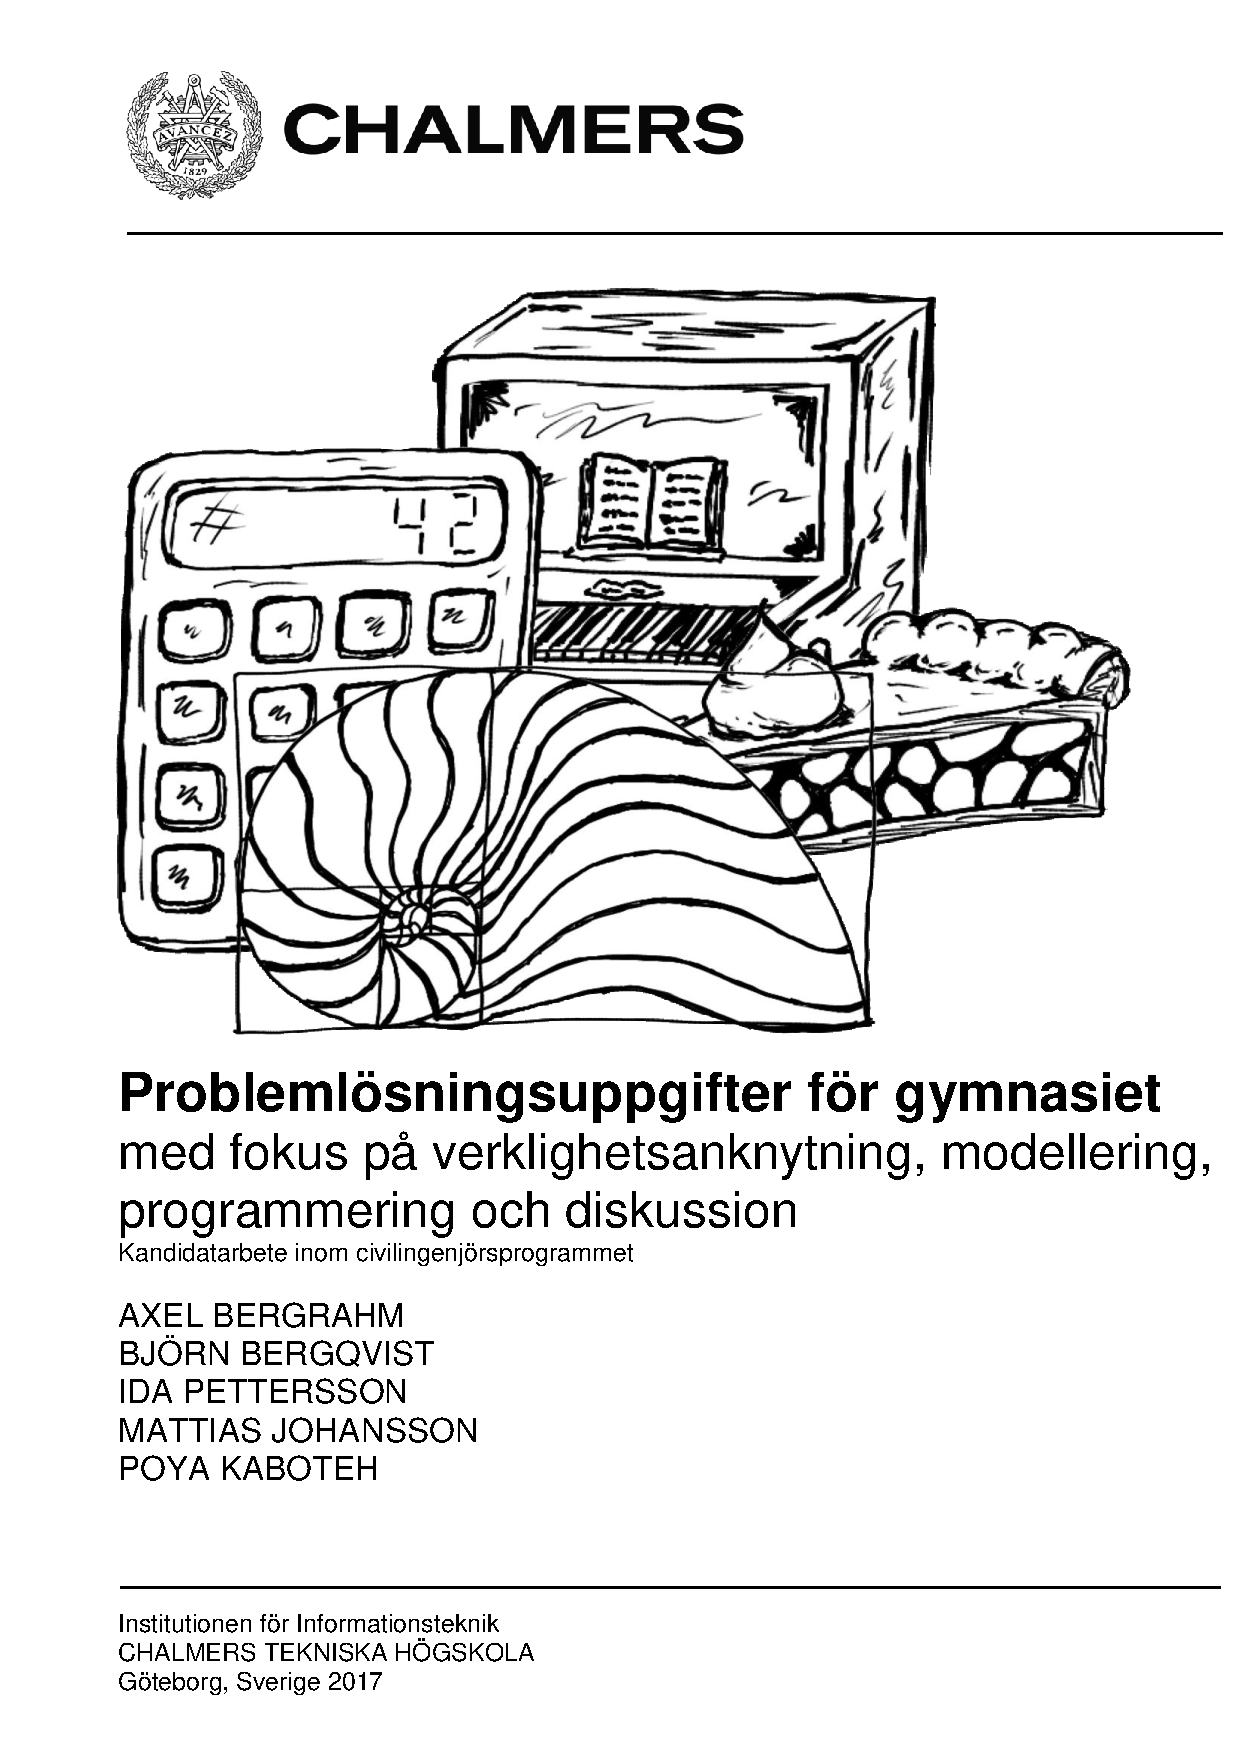
\includepdf{Figures/Framsida.pdf}

\pagenumbering{gobble}

\newpage

\begin{centering}
\Huge
''Tell me and I forget 

Teach me and I remember

Involve me and I learn''

\end{centering}
\bigskip
\begin{centering}

\Large
- Benjamin Franklin

\end{centering}
\newpage

\renewcommand\abstractname{Sammandrag}\begin{abstract}
\noindent \textcolor{Mahogany}{Matematik är ett kärnämne i skolan idag, och anses av de flesta mycket viktigt. Samtidigt är det en vanlig uppfattning att det är svårt, tråkigt och oanvändbart. Med detta projekt vill vi underlätta för lärare att arbeta med problemlösning genom att införa nya typer av matematiska problem för gymnasieskolan,} 
\textcolor{green}{då vår undersökning visade att $91\%$ av gymnasielärare angav att de arbetade med problemlösning, men $42\%$ angav att de hade svårt att hitta bra problem.}
\textcolor{Mahogany}{Huvudsyftet med detta projekt har därför varit att utforma problem för att hjälpa dessa lärare. Problemen är öppna, verklighetsanknutna, ger underlag för diskussion, och ska framför allt ge känslan av att matematik är användbart. Eftersom programmering snart ska införas i skolmatematiken är även en del av problemen konstruerade för att förbereda inför det.}
\textcolor{lila}{Till problemen följer även ett förslag på en komplett lektionsplanering och allt presenteras på en användarvänlig hemsida som ger enkel tillgång för alla lärare som är intresserade.}
\textcolor{green}{De skapade problemen testades även på gymnasieskolor vilket visade att av de 26 svarande ansåg $80\%$ att de lärde sig något och $75\%$ uttryckte på något sätt att problemet var roligt eller meningsfullt. Alla lärare var också nöjda med det problem de testat och ansåg att den information som följde med dem gjorde dem enkla att sätta sig in i.}

% \textcolor{green}{Vår slutsats blev att lärare idag vill inkludera mer problemlösning i undervisningen, men att det inte är lätt att hitta bra problem, samtidigt som en del har tidsbrist. Trots att vi inte lyckades testa problemen i så många klasser som vi hade önskat, så var lärarna och de flesta av eleverna som testade problemen nöjda.}
\end{abstract}

\newpage

\renewcommand\abstractname{Abstract}
\begin{abstract} 
\textcolor{WildStrawberry}{
    DIBS!!!!
}
\end{abstract}

\newpage
 
\tableofcontents

\newpage
\pagenumbering{arabic}

%\section*{Övrigt material som ska in någonstans i rapporten}
    %\subsection{Bör läggas någonstans i diskussionen}

\textcolor{WildStrawberry}{
    Som grupp har vi alla något gemensamt. Vi har alla relativt nyligen genomgått en gymnasieutbildning och tyckes alla komma ihåg att det existerade problem med motivationen på en mängd elever i våra klasser. Internt inom vår grupp så blir det ett stickprov på 5 gymnasieklasser där alla genomgående känner samma sak. Detta stickprov är ju inte alls egentligen något att komma med, det är alldeles för litet för att kunna härleda någon ordentlig slutsats. Men om motivationen på elever i matematiken inte skulle vara ett vanligt problem i gymnasiet skulle vi troligtvis i alla fall haft en person internt som kunde hävda det. Denna observation är dels underlag för vidare undersökning. Gymnasietskolan i Sverige har nya betygssytem och kriterier som lägger en del vikt på problemlösning i matematiken \ref{sec:Forandringar}. Därav kommer syftet med problemen som utformas i detta arbete. Problem som ska öva elever på förmågan att bemöta uppställningar dem inte har svaret på sedan innan och förhoppningsvis medföra större motivation än beräkningar från boken.
}

% exempeltext på syfte...
\textcolor{WildStrawberry}{
    Vi har en bild av att det existerar en svårighet i den svenska matematikundervisningen. Hypotesen lyder att bekvämligheten att hålla fast vid gamla metoder är mer närvarande än föreslagen kursplan vill få ut från undervisningen. Detta projekt har för syfte att testa detta och utforma en mängd problem som skulle uppfylla det syfte som kursplanen vill uppnå. }

\section{Inledning}
    \label{kapitel1} \textcolor{lila}{Matematik är en av de största delarna i skolan både idag och historiskt, vilket bland annat visar sig genom att matematiken är ett kärnämne i både grundskolan och gymnasiet i Sverige. Trots det är det ett ämne som många elever blir stressade över, och som ofta framställs som svårt, tråkigt, oanvändbart och abstrakt \cite{Ignacio&Barona}. En vanlig uppfattning verkar också vara att matematik är ett ämne som bara ett fåtal kan bli bra på \cite{Skolverket03} och ett ständigt återkommande inslag i media är det faktum att matematikkunskapen i Sverige har gått ner under de senaste decennierna \cite{CompareOECD}.
I början av detta projekt hade vi uppfattningen om att skolan till stor del präglas av genomgångar av lärare samt egen räkning i boken, och inkluderar sällan problemlösning i form av verkliga utmaningar som kräver reflektion. Men är det sant? Hur ser undervisningen ut idag och hur har den förändrats genom åren? Vad kan man ändra för att göra den bättre?}

\textcolor{lila}{Detta är något vi bestämt oss för att ta reda på i detta projekt. Vi har därför dels studerat den nuvarande situationen, både med hjälp av källor och egna undersökningar, och vi har även gjort ett bidrag för att försöka förbättra den svenska matematikundervisningen. Detta vill vi göra genom att införa mer problemlösning i gymnasiet, och vi har därför skapat ett antal matematiska problem, tänkta att genomföras på gymnasienivå. Dessa presenteras på en användarvänlig hemsida och ska kunna användas av lärare som vill inkludera mer problemlösning i sin undervisning, men kanske inte har den tid över som det krävs för att planera sådana lektioner.}

\textcolor{lila}{Det som vi framförallt anser att vi kan bidra med till ämnet är vår utgångspunkt som blivande ingenjörer. På så sätt hoppas vi kunna se på problemet från en annan vinkel jämfört med författarna bakom den forskning som redan finns. Dessa är nämligen mer eller mindre uteslutande lärare, pedagoger eller matematiker. Med vår erfarenhet från utbildningar inriktade mot IT och fysik hoppas vi kunna tillföra nya tankar, och skapa problem med en riktig och därmed trovärdig verklighetskoppling. Vi vill att våra problem ska visa på friheten, men också användbarheten, hos matematiken och fokusera på verklighetsanknytning, modellering, programmering och diskussion.}


\section{Matematikundervisning nu och då}
    \textcolor{lila}{Matematik är en av de största delarna i skolan i Sverige idag, vilket bland annat visar sig genom att matematiken är kärnämne i både grundskolan och gymnasiet. Trots det är det ett ämne som många elever blir stressade över, och som ofta framställs som svårt, tråkigt, oanvändbart och abstrakt \cite{Ignacio&Barona}. En vanlig uppfattning verkar också vara att matematik är ett ämne som bara ett fåtal kan bli bra på \cite{Skolverket03} och ett ständigt återkommande inslag i media är det faktum att matematikkunskapen i Sverige har gått ner \cite{CompareOECD}. Men hur ser undervisningen ut idag? Vad kan man ändra för att förbättra dessa resultat?}


    \label{sec:Bakgrund}
    
    % \subsection{Traditionell matematikundervisning}
    %     \label{sec:Traditionellt}
    %     \textcolor{lila}{Den så kallade traditionella undervisningsmetoden består av två delar: \textsl{genomgång} och \textsl{egen räkning} \cite{traditionellMatte}. Det innebär att lektionen börjar med att läraren står framme vid tavlan och går igenom ny teori varefter varje elev individuellt får träna på detta med hjälp av ett stort antal likartade uppgifter. Därefter kan eleverna kontrollera om de gjort rätt genom att jämföra svaret med facit, och därefter gå vidare. Om man får rätt svar på alla uppgifter anser man sig ha gjort det man ska utan att nödvändigtvis ha förstått teorin. Därefter upprepas samma procedur med ett nytt begrepp i centrum.} 
    
\textcolor{lila}{Med den här metoden lär sig eleverna olika matematiska begrepp och metoder, men först efter att det specifika begreppet eller metoden just presenterats. På det faktiska provet, när de själva måste ta reda på vilken metod som ska användas i varje uppgift, blir det betydligt svårare \cite{TheElephant}.}
\textcolor{WildStrawberry}{
    Just på grund av detta så tar man ett steg ifrån verklighetskopplingen och användbarheten av matematiken. När applikationen av teorin blir mekanisk istället för modellerande så tappar teorin syftet och blir mer av ett verktyg för att få ut rätt svar från en fråga. Fokus blir att man utnyttjar korrekt formel och snabbt får feedback från facit, eller andra hjälpmedel, om man fått rätt svar istället för att förstå problemet och dess underliggande moment för vad dem faktiskt innebär. }
    
    \subsection{Hur matematikundervisningen såg ut förr}
        \label{sec:MatteForr}
        %Förändringar i matematikundervisningen

\textcolor{lila}{Den traditionella undervisningen var länge den som mer eller mindre uteslutande användes i Sverige, särskilt i högre åldrar \cite{Namnaren}. Utbildningen i världen har bedrivits på liknande sätt under stor del av matematikens historia. Denna metod kallas \textsl{traditionell undervisning} och är också den metod som ägen länge dominerade svensk undervisning, särskilt i högre åldrar \cite{Namnaren}.}

\textcolor{lila}{Den traditionella undervisningsmetoden kan delas in i två delar: \textsl{genomgång} och \textsl{egen räkning} \cite{traditionellMatte}. Det innebär att lektionen börjar med att läraren står framme vid tavlan och går igenom ny teori varefter varje elev individuellt får träna på detta med hjälp av ett stort antal likartade uppgifter. Därefter kan eleverna kontrollera om de gjort rätt genom att jämföra svaret med facit, och därefter gå vidare. Om man får rätt svar på alla uppgifter anser man sig färdig och går vidare till nästa del. Därefter upprepas samma procedur med ett nytt begrepp i centrum.} 
    
\textcolor{lila}{Med den här metoden lär sig eleverna olika matematiska begrepp och metoder, men först efter att det specifika begreppet eller metoden just presenterats. På det faktiska provet, när de själva måste ta reda på vilken metod som ska användas i varje uppgift, blir det betydligt svårare \cite{TheElephant}.}
\textcolor{green}{
    Den mekaniska räkningen fungerar då inte lika bra och det blir först under provet som elevens självständiga tänkande sätts på prövning.}
    
    %På grund av detta så tar man ett steg ifrån verklighetskopplingen och användbarheten av matematiken. När arbetsmetoden hos eleven blir mekanisk istället för praktisk, då används teorin som ett verktyg för att få ut rätt svar från en fråga. Fokus blir att man utnyttjar korrekt formel och snabbt får feedback från facit eller andra hjälpmedel. }



        
    \subsection{Hur matematikundervisningen har förändrats}
        \label{sec:Forandringar}
        \textcolor{lila}{På senare år har man börjat att aktivt se över hur undervisningsmetoden skulle kunna förbättras. Intresset för problemlösning vaknade internationellt under 1980-talet \cite{80-talet}, och nu är ämnet mycket aktuellt i didaktiska sammanhang. År 2011 infördes en ny och uppdaterad kursplan för gymnasiet, GY11, som bland annat påverkade matematiken. Jämfört med de tidigare kursplanerna från 2000 fanns det ett antal viktiga ändringar som gällde alla de olika matematikkurserna. 
Dessa förändringar diskuteras i en jämförelse mellan de båda kursplanerna \cite{GY00-GY11}, där den nya anges lägga mer fokus på att kurserna ska anpassas efter varje program och inriktning. På så sätt plockas verklighetsanknytningen upp på ett tydligare sätt. Man ska alltså lära sig hur matematik kan användas i vardagssammanhang som exempelvis att betala räkningar, men även i mer specifika situationer beroende på vad man kan behöva i yrkeslivet alternativt vidareutbildningen efter gymnasiet. 
Samma källa tar även upp en annan viktig ändring som gäller problemlösning. Detta hade ingått även tidigare, men då bara som ett av \textsl{målen}. Nu ska det även användas som \textsl{medel} för inlärning av andra mål. I GY11 poängteras också att undervisningen ska varieras och innehålla undersökande aktiviteter.}

\textcolor{lila}{För att dessa förändringar ska kunna implementeras på ett så bra sätt som möjligt har man också gjort en stor satsning genom att fortbilda alla lärare. Detta har gjorts genom \textsl{Matematiklyftet}, som är en kompetensutveckling i didaktik för matematiklärare \cite{Namnaren}, och den största satsning som någonsin gjorts i ett enskilt ämne i Sverige \cite{mattelyftet}. Här belyses den kommunicerande, reflekterande samt undersökande delen av matematiken som återfinns i samband med problemlösning.}
            
\textcolor{lila}{Problemlösning är alltså ett mycket aktuellt ämne, som man lägger mycket resurser på att införa i matematikundervisningen. Det är dock en mycket stor förändring att genomföra och tar därför, som alla andra stora förändringar, tid. Många lärare tycker också att det är svårt att hinna med problemlösning vid sidan av det material som redan ska täckas enligt kursplanen \cite{2016Senare}.}

%Även de lärare som arbetar aktivt med att införa mer problemlösning stöter på ett viss motstånd. Kanske är det för att flesta elever är vana vid den traditionella undervisningen. Eleverna förväntar sig då att lärarna ska tala om precis hur man ska göra och vad som är rätt och fel. De gamla vanorna kan alltså sitta djupt hos både elever och lärare, och vara svåra att ändra.}

\textcolor{lila}{I mars i år (2017) beslutades att skolan även ska verka för att ``stärka elevernas digitala kompetens'' \cite{regeringen}. För gymnasiematematiken innebär detta att användingen av digitala verktyg ska bli mer central i matematikundervisningen och programmering ska användas för att lösa matematiska problem \cite{itiskolan}. Även här ska det genomföras fortbildning av lärare \cite{prog_utbildning}. Ett rimligt antagande är dock att även denna övergång kommer bli svår och ta lång tid att genomföra.}
        
    \subsection{Matematikundervisningen idag och gapet till arbetsliv och högskola}
        \textcolor{WildStrawberry}{
    Den svenska matematikundervisning innefattar i stora drag att en lärare lär ut ett eller flera teoretiska begrepp inför sin klass och sedan ska klassen repetera dessa nya begrepp tills det sitter i muskelminnet. Repetitionen i sin tur, kommer troligtvis innebära att eleven sitter med en lärobok som har en mängd definierade uppgifter där den nya teorin ska appliceras. Detta moment kommer att hamna i en sluten loop tills det är dags för det stora provet där man testar alla begrepp man tidigare gått igenom.
}

%ny rubrik? problemet?
%\textcolor{WildStrawberry}{
 %   Problemet med denna typen av undervisning är att eleven inte behöver känna igen det underliggande problemet, eleven kommer undan med att memorera hur en formel ser ut – utan att nödvändigtvis behöva förstå vad formeln gör. Inte för att testa förmågan att memorera saker är dåligt, men just på grund av detta så tar man ett steg ifrån verklighetskopplingen och användbarheten av matematiken. När applikationen av teorin blir mekanisk istället för modellerande så tappar teorin syftet och blir mer av ett verktyg för att få ut rätt svar från en fråga. Fokus blir att man utnyttjar korrekt formel och snabbt får feedback från facit, eller andra hjälpmedel, om man fått rätt svar istället för att förstå problemet och dess underliggande moment för vad dem faktiskt innebär. }


%vad matematiken & skola bör lära ut

% från intervju med Gymnasieelev när ställd frågan "blir ni skolade på hur man löser problem eller är problemlösningen ett vanligt matteproblem som är maskerat i text?": 
%" Mestadels det senare, vi gör problemlösningen i matten så man ska försöka hitta den användbara infon och lösa matteproblemet. Jag tar lite svårare matte men samma kurs som andra så min grupp får lite mer roliga problem där man måste använda logik i kombination med algebraisk matte...

% Men generellt så löser man mest maskerade matte problem"

\textcolor{WildStrawberry}{
    Enligt den nya läroplanen för matematik, som infördes 2011, så ska matematiken beröra problemlösning på så vis att man ska lära sig behärska sunt resonemang och logik. Eleven ska kunna bemöta uppställda situationer med metodik och kunna modellera en lösning från given information. Givetvis låter detta bra, men vad har egentligen ändrats - Från vår undersökning så får elever uppgifter, precis som i läroboken, maskerade i en kort saga som ska simulera ett problem. Reglerna är ofta tydliga och tanken är att man hittar siffrorna i texten och använder korrekt formel som man fått på undervisningen. 
}

%(citat från intervju? hittas i .tex filen ovanför stycket).
% HEEEJ :D ändra precis som du könner är swag! jag bara får ut något på papper just nu :)
% Haha, det är bra att du skriver! :D Tänkte bara hjälpa till när jag såg det och kunde :)
% Super! :D All hjälp är toppen, tror du jag tänker rätt på denna sektion? den är ju mycket lik den om traditionell skola
% Ja... Det är jag lite osäker på... Funderar på om det inte är bättre att du försöker lägga in delar av det du skrivit i det stycket... Det är ju också svårt att påstå saker utan källor, så det måste vi försöka vara noga med. 
% AA exakt! Men på sätt och vis har vi en "intervju" med en duktig matte-student. Som är en källa. Dock en källa 
% - intJeo a,l ol skoor.
% wow :D

% Det är nog också mer relevant till "matematiken idag". Det existerar en bekvämlighetsfaktor just på grund av tiden är bristande och därför är det najs att använda sig av färdiga problem som inte har mycket tanke bakom sig. - Eleven får övning och "problemlösning (läsförståelse)"

% :( 
% okej <3 <3<3<3<3 till synes borta :smirk:
% Haha, förlåt xp
% Tänket bara säga att vi ju kan använda det som att vi vet att det händer, men inte som att det alltid är så. Vi kan också gå in mer på att det är svårt att hinna med, och ta in lite mer från planeringsrapporten. Precis, eller inte från lärarnas håll i alla fall ;)
% Ska vi ta bort detta nu kanske :p
%Fixade! ;) Inte helt borta i alla fall!

%Här kommer några bra dåliga problemlösningsuppgifter ifrån \cite{matte5000} - MVH Björn

%Följande är en a uppgift, dvs en lätt uppgift:
\begin{displayquote}
\textcolor{turkos}{Marcus läser en bok som innehåller 420 sidor. Mellan kl 19.45 och 20.15 läser han 14 sidor. \\
Hur lång tid tar det att lösa hela boken?}
\end{displayquote}

%Svar

%Detta är en b-uppgift
\begin{displayquote}
\textcolor{turkos}{Jonas kör sin bil samma sträcka varje dag. Sträckan är en mil och Jonas brukar köra med hastigheten 90 $km/h$ en dag kör han sträckan med 100 $km/h$. \\
Hur många sekunder ''tjänar'' Jonas på det?}
\end{displayquote}

%Svar

%Följande två uppgifter är c-uppgifter, dvs de svåraste. 

\begin{displayquote}
\textcolor{turkos}{Vilket tal är x?\\
\( 2*5^x + 3*5^x = 25^{12} \)}
\end{displayquote}

%Svar

\begin{displayquote}
\textcolor{turkos}{En sandstrand är 2km lång, 30 m bred och 3 m djup. \\
Vi antar att ett sandkort ryms inom ett kubiskt område med sidan 0,2 mm.\\
Hur många sandkorn finns på stranden?}
\end{displayquote}

%Svar

%Samtliga fyra uppgifter har tagits från delkapitel 1.4 Problemlösning, som är del av 1 Aritmetik - Om tal. Finns liknande uppgifter i kapitlen om 2.2 Procentuellea förändringar och 3.2 Linjära ekvationer och olikheter. Dock saknas helt uppgifter om problemlösning för Geometri, Sannolikhetslära och statistik, samt Grafer och funktioner. 
        \label{sec:matteidag}
        
%    \subsection{Gruppindelning}
%        \label{sec:Gruppindelning}
%        \textcolor{turkos} {Det är vanligt att dela upp elever efter hur snabbt de anses lösa uppgifter. Elever som löser uppgifter snabbt grupperas med andra elever som löser uppgifter ungefär lika snabbt, och det samma gäller elever som anses lösa uppgifter långsamt och en grupp för elever som ligger mellan de två andra grupperna \cite{Skolverket03}. }


\section{Syfte}
    \textcolor{lila}{Med det här projektet vill vi bidra till att införa mer problemlösning i undervisningen, eftersom vi innan detta arbete hade uppfattningen att detta inte inkluderas tillräckligt. Projektets syfte är därför att skapa matematiska problem med förslag på tillhörande lektionsplanering som lärare kan använda i sin undervisning.}
\textcolor{Mahogany}{På så sätt vill vi minimera den tid som lärarna behöver lägga på lektionsplanering och på så sätt göra det lättare att variera kursboksmaterialet med mer problemlösning.} 
\textcolor{lila}{Med dessa uppgifter vill vi visa matematikens många sidor och ge eleverna en känsla för hur relevant matematiken är, och hur den kan användas. Problemen ska uppmuntra eleverna till att diskutera matematik och upptäcka friheten och kreativiteten som finns i matematiken. Flera av problemen bygger också på programmering, några direkt och ett mer indirekt. Med problemens tydliga struktur hoppas vi också kunna inspirera och förenkla för lärare som vill utveckla egna problemlösningslektioner utifrån egna idéer.}

\textcolor{lila}{Vi ville även undersöka om vår ursprungliga hypotes om problemlösning i undervisningen, som nämndes i bakgrunden (\ref{sec:Bakgrund}), stämmer samt ifall det finns några specifika faktorer som motverkar detta. I så fall ville vi anpassa projektet efter de motverkande faktorer som uppdagades, så att vi kan bidra till att minska dessa. För att göra det enkelt för lärare att hitta och använda problemen ska de presenteras på en webbplats, tillsammans med övrig information om hur de kan användas.}

%\textcolor{lila}{Syftet är att förse lärarna med problemlösninguppgifter, som presenteras i form av en hel lektionsplanering. På så sätt hoppas vi kunna hjälpa de lärare som tycker att det är svårt att hitta bra uppgifter alternativt inte anser sig ha tid till att planera lektionen till den grad som behövs om man frångår boken. Planeringen är dock tänkt enbart som en riktlinje, och varje lärare får själv avgöra hur mycket av den dom vill följa, samt lägga till moment som de anser passande.}

\subsection{Varför gymnasiet?}
\textcolor{lila}{
    Vi har valt att rikta in detta arbete specifikt mot gymnasiematematik. Även om vi tror att det är viktigt att utveckla matematiken på likande sätt i alla åldrar, så har vi valt en mindre målgrupp för att kunna genomföra arbetet på ett bra sätt och med ett användbart resultat. }
    
\textcolor{lila}{
    Det finns flera anledningar till varför valet av målgrupp föll på just gymnasiet. Dels finns det forskning som visar att en förändring i matematiskt tänkande, tvärtom vad man kan tro, är bättre att införa i den senare delen av skolan \cite{TheElephant}. Det är lätt att tro att en ändring som införs tidigt fortplantar sig till efterföljande matematikkunskaper, men så är det alltså inte i allmänhet. Gymnasiet är också sista steget innan man eventuellt fortsätter till universitet, högskola eller arbetsliv där man förväntas lösa problem utan att ha alla fakta och metoder givna på förhand. En försmak på detta är något som vi saknade i gymnasiet, och hoppas därför kunna ge till andra.}
    
\textcolor{lila}{        
    På gymnasiet har glädjen för att lära sig matematik, som är vanligt i de yngre åldrarna, för många elever till stor del ersatts utav rena prestationsmål \cite{Skolverket03}. Vi hoppas kunna visa en annan sida utav matematiken som väcker den glädjen igen.}
   
        

%   Borttaget ---
% Anledningen till varför vi inriktat oss mot gymnasiet är dels på grund av anledningen att vi internt känner att det i alla fall har existerat ett problem och vi tror att oavsett hur en kursplan förändras så kommer arbetet vara lika omotiverande så länge uppgifterna inte förändras. Man kan inte klandra lärarna och säga att de inte försöker inspirera och uppmuntra till en god miljö. Med ett förtroende för lärarnas kompetens så anser vi att feletproblemet inte ligger hos dem, utan det befinner sig i naturen av uppgifternas enformighet och fantasilöshet \ref{sec:Verklighetsanknytning}. Lärarna har för lite tid för att skapa intressanta uppgifter till sina elever och måste lägga tiden på allt annat omkring som finns med i kursplanen. Tillsynes verkar det inte heller finnas många som jobbar med att ta fram utmanande problem som passar en bredvid målgrupp av både högt - och -lågt presterande studenter. Målgruppen på sådana problem brukar ha en inriktning mot den ena eller andra gruppen av elever.}
    
    % \subsection{Problembank} \todo{!}
    %     \textcolor{Mahogany}{
    %Som nämnts i kapitel \ref{sec:Forandringar} så saknas hjälp med hur man både lär ut samt inkluderar mer problemlösning i undervisningen. 
    Genom att tillhandahålla lärare allmän information kring hur problemen som utformats i detta projekt ska utföras och vad fokus ska ligga på, så minimeras den tid som lärare behöver lägga för att planera lektionen, men ändå variera kursboksmaterialet med mer problemlösning.
}

% Från "Undervisning i syfte att stödja och utveckla samtliga elevers individuella matematiska förmåga": I dagsläget används som beskrivits ovan läromedlet Matematikboken för grundskolans senare år X (Undvall m.fl. 2001a) i undervisningen i år 7. Detta läromedel innehåller många uppgifter, som också skulle kunna användas i arbetet inom ramen för utökad undervisningstid i matematik. Denna typ av uppgifter finner läsaren oftast under speciella rubriker såsom ”TEMA”, ”Träna problemlösning” respektive ”Lite av varje”, som bland annat innehåller olika typer av fördjupande huvudräknings-, grupp- samt diskussionsuppgifter där eleverna ges möjlighet att reflektera över matematiskt tänkande både enskilt och i grupp. Då dessa uppgifter är lättillgängliga att använda som resursuppgifter i den ordinarie undervisningen i matematik tre lektioner i veckan, speciellt då elevernas kompetens att självständigt ta sig an annorlunda uppgifter i matematik successivt kommer att öka tack vare det utökade matematikarbetet under veckans fjärde matematiktimme, är det önskvärt att i första hand uppgifter från annan litteratur än det ordinarie läromedlet användas för elevernas arbete under veckans fjärde matematiklektion. För undervisande lärare är det dock tidskrävande att åstadkomma variation med stor bredd, varför en gemensam planering med förberedda uppgifter kraftigt underlättar arbetet så att mer kraft kan ägnas åt projektets genomförande.
    
    \subsection{Webbplatsens roll}
        \textcolor{Mahogany}{Webbplatsen är ett sätt att förmedla de problem som vi utformat till fler än de som vi testar problemen med. Med hjälp av webbplatsen kan vi ge både lärare och elever möjligheten att ta del av våra problem när de vill och känner att de har tid över.
%Det hjälper oss också att få spridning på de problem som vi utformat, kanske tyckte de att problemen var givande och delar med sig av sidan till en kollega, som kanske i sin tur gör samma sak.
I slutändan så hoppas vi helt enkelt att så många som möjligt kan ha hjälp av de problem som vi utformat.}

\textcolor{Mahogany}{Webbplatsen är också det som kommer att leva kvar efter projektet, så vi har valt att inkludera en kort beskrivning om oss och vårt arbete, samt en liten informativ text till lärare med vad vi vill uppnå med våra problem och hur vi tänkt att de ska utföras.}

\textcolor{WildStrawberry}{
    Med en färdig webbplats så skulle också projektet lätt kunna vidareutvecklas i framtiden. Det enda som skulle krävas av de som utvecklar vidare på projektet är några få instruktioner på hur man lägger in information för nya problem. Den underliggande arkitekturen tillåter utbyggnad på så pass enkelt vis att man kan lägga mer fokus på annat, exempelvis att utveckla problem.
    }
% saker att skriva om: definiera ett problem bättre, matematisk modellering, öppna problem, undersökande arbetssätt
\section{Varför är problemlösning viktigt?}
    \label{sec:Teori}
    \textcolor{lila}{För att förstå detta måste man först fundera på vad problemlösning egentligen är, vad det innebär och hur det kan användas. Detta kapitel förklarar därför begreppet och vilka fördelar som förljer med denna typ av undervisning. Eftersom problemlösning ofta leder till intressanta diskussioner och därmed med fördel genomförs i grupp beskrivs även dessa delar mer ingående. Kapitlet avslutas med att förklara hur problemlösning kan gynna alla elever, oavsett nivå.}
        
    \subsection{Vad är problemlösning?}
        \label{sec:problemdef}
        %\textcolor{Mahogany}{Vi definierar ett problem som en uppgift som man på förhand inte vet hur man ska lösa. }

% Vad är inte problemlösning
\textcolor{WildStrawberry}{
    Komplexiteten med att definiera vad ett problem är ligger i att det existerar olika syften med vad ett problem vill få ut från den som testas. Vissa problem vill att du hittar x - kan du hitta x? Andra problem kanske inte har ett exakt svar - tillvägagångssättet när man försöker lösa problemet är det som är utvecklande. Det vi vill ta ställning för är att en ''lös ut x''-uppgift som är dekorerad i en \textit{saga} skapar inte ett intressant problem och kunde lika väl varit den vanliga ''vad är x''-övningen. 
}

% Vad är problemlösning
\textcolor{WildStrawberry}{
    Det finns en mängd olika infallsvinklar man kan ta för att definiera \textit{ett problem}. Den som testas bör behöva fundera på vad som är viktigt i en given situation och skapa egen modellering av verkligheten. Ett problem bör skapa ett behov för teorin som kan appliceras och därav förhoppningsvis härleda för en djupare förståelse till varför teorin fungerar. När man fått fundera på hur man \textit{kan} gå till väga för att lösa problem innan man får underlaget så binder man en starkare koppling till materialet och bör därför komma ihåg det bättre\todo{källa}. Men vi vill definiera att \textit{ett problem} är en form av uppgift där man får arbeta med en situation eller uppställning som man inte kan svaret till på förhand.
}


    \textcolor{lila}{Denna definition gör det på sätt och vis mycket svårt att skapa ett problem, eftersom den innebär att en uppgift som är ett problem för en person, kan vara en ren standarduppgift för någon annan. Definitionen innebär också att problemlösning är ett mycket brett område. Nedan presenteras några viktiga delar som, tillsammans eller var och en för sig, kan lyftas fram i ett bra problem.}
    
    \textcolor{lila}{Till att börja med kräver problemlösning ett \textsl{undersökande arbetssätt}. det handlar om att analysera problemet och bryta ner det i mindre delar, och därefter hantera varje del var för sig. Ofta måste man prova sig fram med olika lösningsmetoder innan man hittar en som fungerar.}
        
    \textcolor{lila}{En vanlig form av problemlösning är genom att använda \textsl{öppna problem}. Det innebär ett  problem till vilket det finns flera olika möjliga lösningsgångar för att hitta ett svar, och detta svar behöver inte heller vara unikt utan kan variera beroende på vilka antaganden som gjorts.}

    \textcolor{lila}{En annan viktig del är att kunna översätta ett problem i \textsl{matematiska modeller}. Detta är en nyttig förmåga att besitta i många olika sammanhang, även i arbetslivet~\cite{TheElephant}. Det är också minst lika viktigt att kunna granska en modell med kritisk blick, och fundera på i vilka sammanhang den gäller och när den leder till orimliga resultat.}
    
    \subsection{Polya's fyra steg}
        \label{sec:polya}
        \textcolor{Mahogany}{
    Redan under 1940-tal så framhäver Polya i \textsl{How to solve it} \cite{Polya} behovet av iteration, att man alltid ändrar sitt synsätt, vilket också är ett viktigt steg i de \textsl{fyra faser} som han har tagit fram för hur man löser ett problem.
    Det första är att \textsl{förstå} problemet, vad som efterfrågas. Det andra är att kunna koppla olika element i problemet och se hur det okända är länkat till den data man har, för att i tredje steget genomföra problemet. 
    Det andra steget kan dock oftast i traditionella matematikuppgifter vara väldigt uppenbart och det finns en risk att man redan i detta steget får fram ett svar och går vidare. 
    Fjärde steget handlar om att man tittar tillbaka på vad man har fått fram och diskuterar resultatet. Detta är också det som kommer att läggas betydligt stor vikt på vid utformandet av problemen som utvecklats i detta projekt, nämligen \textsl{diskussion}.
}

\textcolor{Mahogany}{
    Vidare beskriver Polya mer ingående för det fjärde steget att elever tenderar att gå vidare och göra annat efter att ha kommit fram till ett svar, och att eleverna då missar en viktig fas. Genom att utvärdera sina resultat och framför allt \textsl{processen} att komma fram till resultatet, ges det utrymme för personen att att stärka sin kunskap och utveckla deras förmåga att lösa problem. Han menar vidare att det alltid finns sätt att förbättra sin lösning men också sin förståelse för lösningen.
}
        
    \subsection{Problembaserat lärande}
        \label{sec:pbl}
        \textcolor{green}{Den undervisningsmetod som används i samband med de flesta av de framtagna problemen kallas för \textit{problembaserat lärande}, förkortat \textit{PBL}. Metoden går ut på att lära sig problemlösning genom att lösa verklighetsanknutna och ostrukturerade problem. Med ostrukturerade problem menas att uppgiften inte har och inte indikerar några bestämda sekvensiella steg som den ska lösas i. Problemen kan lösas på olika sätt och lösningen är tänkt att vara oförutsägbar. Tanken är att arbetet med verkliga problem ska ge möjlighet att tillämpa de matematiska teorier som är relevanta för just dessa problem. PBL nyttjar människans medfödda förmåga och nyfikenhet att lära sig, vilket ger en djupare förståelse för den kunskap som lärs in \cite{PBLdefinition} \cite{djupareKunskapPBL}.} \textcolor{Mahogany}{Alla gynnas dock inte av PBL. Studier visar bland annat att elever i grundskolan med större pedagogiska behov kan ha svårt att arbeta under denna undervisningsmetod. Framför allt så handlar det om svårigheter att arbeta självständigt~\cite{Johansson} och söka egen information~\cite{Carlsson}. Den senare studien visar även att PBL är mer resurskrävnade än traditionall undervisning som arbetsmetod för lärare.}

\textcolor{green}{Det som kan ses som motsatsen till PBL är \textit{deduktiv inlärning}. Deduktiv inlärning är den undervisningsmetod som den traditionella matematikundervisningen använder sig av, att i första hand lära ut teorier för att sedan tillämpa dessa på lämpliga uppgifter ~\cite{deduktivInlärning}.}

%Om ett par elever lyckas komma på en lösning, eller del av en lösning, till ett problem så kan det bidra till att göra matematiken mindre främmande. Om en viss del av den teori som lärs ut i matematiken blir i form av egen utforskning, och att man lyckas komma en bit eller hela vägen, så kan denna belöning agera mycket motiverande~\cite{TheElephant}. Dock inte uteslutande då varje individ inte har samma målsättningar samt motivation.} \textcolor{lila}{Men genom att utifrån en fråga upptäcka ett matematiskt begrepp ges detta automatiskt ett sammanhang och eleverna inser att det är användbart. På samma sätt är det motiverande för elever att känna att de äger problemet, det vill säga att de själva får forma problemet i form av frågeställning och bakgrundsinformation.} %Mycket av den teori som elever idag får lära sig under sin skolgång har kommit till under processen att lösa verkliga problem. Det är alltså verkliga problem som har lett till dessa teorier, som sedan har blivit formler. Att komma till denna insikten kan visa sig vara ett kraftfullt verktyg för studentens delaktighet i sin utbildning.
%
%
%
%Problembaserat lärande är den pedagogik som de flesta av våra uppgifter använder sig av.
%INQUIRY BASED LEARNING...
%Det är den karaktär våra problem har
%Vad är fördelen med det?
%Vi tror att eleverna får djupare förståelse för teori, om de först får se verkliga scenarion som den kan appliceras på
%matten känns inte irrelevant, utan kan lösa riktiga problem
%matematiken får även fler dimensioner än att vara ute efter ett enda rätt svar Detta eftersom uppgifterna är gjorda på ett sätt där de på precis samma sätt som många problem i verkliga inte har "ett rätt svar" utan snarare ska estimeras och optimeras. 
%Dag Wedellin använder i sin kurs x denna metod och har fått denna respons - detta tycker vi talar för att denna metod är bättre än den traditionella
%
%
\textcolor{turkos}{Vidare skriver Daniel Willingham i sin bok \textsl{Why Students Don't Like School?} om vikten utav repetition för inlärning \cite{WhyDontStudents}. Enligt Willingham så är faktabaserad kunskap starkt sammankopplat till kritiskt tänkande så som problemlösning, och för att uppnå den kunskapen krävs repetition. Han skriver att övning hjälper människor att överföra information till nya situationer, att kunna ta gammal kunskap och applicera den i nya situationer är en viktig del utav problemlösning. Willingham beskriver även skillnaden mellan noviser och experter (till exempel matematiker) sätt att arbeta på, och att det inte går att förvänta sig att novisen ska lösa samma problem som experten tas sig an då de saknar samma kunskapsbas. Istället anser han att man kan låta elever inspireras utav experternas arbete utan att faktiskt låta dem göra samma sak. } \todo{Funkar det här?}


%\textcolor{turkos}{Daniel Willingham beskriver i sin bok \textsl{Why Students Don't Like School?} att för att kunna tänka som en expert så behöver man grundläggande kunskap, och det enda sättet att få den grundkunskapen är genom repetition \cite{WhyDontStudents}. }

% Practice helps transfer information to new situations


        
    \subsection{Arbeta i grupp}
        \label{sec:Arbetaigrupp}
        \textcolor{turkos} {
Att låta elever arbeta med problemlösning i små grupper om två till fyra personer leder till att varje elev ges möjlighet att diskutera och reflektera angående problemet. Eleverna får prata om sina idéer till lösningar, lyssna på andra elevers idéer, samt även ges möjlighet att fråga, kritisera och bemöta kritik på ett positivt sätt. När eleverna får förklara sina tankar leder det till ökad matematiksförståelse. \cite{RikaProblem}
}

\textcolor{turkos} {
Som tidigare nämnts i \ref{sec:Gruppindelning} är det vanligt att skolor delar in elever i grupper efter deras matematikfärdigheter, dock hävdar både Boaler \cite{TheElephant} och Rika matematiska problem \cite{RikaProblem} att det är bättre med heterogena grupper vad det gäller matematikkunskap. I blandade grupper där man arbetar efter metoder anpassade för dem får elever lära av varandra vilket leder till ett mer rättvist klassrum enligt Boaler \cite{TheElephant}. 
}

\textcolor{turkos} {
Rika matematiska problem rekommenderar att läraren blandar medelpresterande elever med högepresterande eller lågpresterande elever när man gör gruppindelningen, men varnar samtidigt för att inte göra grupperna extremt homogena eller heterogena\cite{RikaProblem}.
}

% I blandade grupper hjälper elever varandra vilket leder till fina ord som equality och allt blir bättre - Jo Boaler

% Även Rikaproblem rekommenderar att man blandar medelpresterande elever med högepresterande eller lågpresterande elever när man gör grupp indelningen, men varnar samtidigt för att inte göra grupperna extremt homogena eller heterogena. 


\textcolor{turkos} {
En negativ aspekt med grupparbete är att vissa elever kan bli sittande passivt medan resten av gruppen löser uppgiften åt dem\cite{RikaProblem}. Detta problemet kan rimligen antas bli värre ju större gruppen blir. 
}

%Bygga en rödtråd till förra kapitlet genom Japanska skolan. 



% Problemlösning i grupp anses vara roligare än vanliga mattelektion - Skolverket

% Saknas något om olika gruppstorlekar, samt nackdelar

% En studie visar att 2 är bättre än 1 förrutom för de allra bästa eleverna där det är ungefär lika bra, men 3-5 är strängt bättre. Den säger även att testpersonerna hade något roligare när det arbetade individuellt.

%Negativt - Om man börjar med grupparbete så kan vissa elever bli sittande passivt medan resten av gruppen löser uppgiften åt dem. - Rikaproblem



% Grupper bör ligga på 2-4 elever, eftersom det i en sådan grupp ger alla elever möjlighet att delta i diskussioner - Rika problem 

% Gruppering efter färdigheter är vanligt, enligt skolverket. 
        
    \subsection{Diskussion och kommunikation inom matematik}
        \textcolor{turkos} {
Givande diskussioner kan få elever att inse att det är tillåtet att ha egna idéer och tankar kring matematik, ett ämne som annars ofta upplevs handla om att följa regler. När elever diskuterar problem med varandra så lär de av varandra, och kan ofta uttrycka sig på ett sätt som kan göra det lättare för dem att förstå än vad ofta läraren kan. \cite{TheElephant}
}

\textcolor{turkos} {Faktum är att diskussion är så viktigt för bra problemlösning att Hagland m.fl. skriver, i deras bok Rika matematiska problem, att den viktigaste skillnaden mellan ett vanligt problem och vad de kallar ett rikt problem är att det rika problemet leder till diskussion \cite{RikaProblem}. Även Skolverket lyfter att matematikundervisning där elevers egna lösningstratergier diskuteras leder till mycket positiva resultat och ökar elevers lust att lära\cite{Skolverket03}.}

\textcolor{turkos}{I Rika matematiska problem beskrivs även vikten av ha en avslutande klassdiskussion \cite{RikaProblem}. Anledningen till att boken lägger vikt vid diskussion just på slutet är att alla elever tid att jobba med problemet, även om alla kanske inte har löst det, och kan därmed bidra till diskussionen. Även läraren har haft möjlighet att bilda sig en uppfattning om vilka metoder eleverna har använt för att lösa problemen och kan därmed leda diskussionen och ta upp intressanta idéer som uppstått i klassen och lyfta dem till resterande elever.}

\textcolor{turkos} {
Ett land som tas upp som ett exempel på god matematikundervisning av både Skolverket och Boaler är Japan \cite{TheElephant}\cite{Skolverket03}. Skolverket beskriver hur det i Japan läggs stor vikt vid att efter eleverna löst ett problem så ska de dela med sig utav sina lösningar och diskutera dem med varandra. Där används diskussionen som en utgångspunkt för att läraren ska kunna lyfta viktiga aspekter ur deras lösningar och tillvägagångssätt.}

% Rika problem är problem som leder till diskussion

% Ger chans att lyfta sina egna idéer och utveckla dem. 

% Diskussion leder till öka lust att lära. 

% Japanska skolan lägger fokus på diskussion och lyfts som ett föredöme av både skolverket och Jo Boaler 

% Tar upp strukturen med diskussion före och efter elever får lösa problemet. 


% Skriv något om att det är bra att reflektera efter man har gjort en uppgift. 
        \label{sec:Diskussion}
    
    \subsection{Utdrag ur lärobok}
        \input{Sections/Teori/Utdrag.tex}
        
    \subsection{Verklighetsanknytning i matematiken}
        \label{sec:Verklighetsanknytning}
        \textcolor{lila}{En vanlig uppfattning är att det finns för lite verklighetsanknytning i matematiken som lärs ut idag \cite{TheElephant}. Mot denna bakgrund är det lätt att förstå att elever kan tolka ämnet som onödigt och irrelevant, vilket förklarar varför det är så viktigt att eleverna upplever uppgifterna som relevanta.}

\textcolor{lila}{Detta är ett faktum som många kursboksförfattare tagit fasta på, men tyvärr uppnår dessa försök inte alltid målet. Ofta känns den så kallade verklighetsanknytningen forcerad, och det blir snarare dåligt förklädda standarduppgifter än faktiska problem som man kan föreställa sig att någon skulle vilja lösa. Detta riskerar att ge eleverna en känsla av att matematik inte är användbart, eftersom de får se så få exempel från dess verkliga användningsområden.
I vissa fall har man också tänkt för mycket på att den relevanta matematiken ska finnas med i uppgiften, vilket kan leda till att rimligheten blir lidande. Jo Boaler beskriver det som att eleverna inser att det finns ett speciellt ''matteland'', där det vanliga sunda förnuftet inte längre gäller \cite{TheElephant}.}
    
\textcolor{lila}{De textuppgifter som skrivs  i kursböcker med avsikt att införa en verklighetsanknytning kan också enligt vår erfarenhet i många fall brytas ner till standardproblem enbart genom att plocka ut siffrorna ur texten. På så sätt kan man också ofta bortse från den verklighetsanknytning som eventuellt finns i uppgifterna.}

\textcolor{lila}{Det verkar alltså vara viktigt med verkligehtsanknytning i matematiken, så att eleverna kan relatera till uppgiften och få känslan av att matematik är viktigt och användbart.} \textcolor{Mahogany}{Dock framhäver Lockhart i sin \textsl{A Mathematician's Lament} \cite{lockhart} behovet av att elever ska få utforska matematiken och att man ska försöka underbygga deras fantasi, snarare än att låsa alla problem vid verklighetsanknytning. Alltså bör uppgifter med verklighetsanknytning inte bara framhäva att matematik är användbart i det verkliga livet, utan även få eleven att känna att den är användbar.}
        
    \subsection{Göra eleverna delaktiga i undervisningen}
        \label{sec:delaktighet}
        
\label{sec:delaktighet}
\textcolor{WildStrawberry}{
    Om ett par elever lyckas komma på en lösning, eller del av en lösning, till ett problem så kan det bidra till att göra matematiken mindre främmande. Om en viss del av den teori som lärs ut i matematiken blir i form av egen utforskning, och att man lyckas komma en bit eller hela vägen, så kan denna belöning agera mycket motiverande~\cite{TheElephant}. Dock inte uteslutande då varje individ inte har samma målsättningar samt motivation.} \textcolor{lila}{Men genom att utifrån en fråga upptäcka ett matematiskt begrepp ges detta automatiskt ett sammanhang och eleverna inser att det är användbart. På samma sätt är det motiverande för elever att känna att de äger problemet, det vill säga att de själva får forma problemet i form av frågeställning och bakgrundsinformation.}
    
    \textcolor{WildStrawberry}{
        All teori som en elev utsätts för under sin skolgång har varit ''verkliga'' problem som en gång inte varit färdiga formler eller modeller, som nu går att utnyttja. Att komma till denna insikten kan visa sig vara ett kraftfullt verktyg för studentens delaktighet i sin utbildning. Förmågan att ifrågasätta och kunna bemöta situationer objektivt ger individer en större frihet att förstå, utforska och utmana existerande begrepp.}
        
        %Mycket av den teori som elever idag får lära sig under sin skolgång har kommit till under processen att lösa verkliga problem. Det är alltså verkliga problem som har lett till dessa teorier, som sedan har blivit formler. Att komma till denna insikten kan visa sig vara ett kraftfullt verktyg för studentens delaktighet i sin utbildning.
            
        
    \subsection{Programmering: Tillämpad problemlösning}
        \label{sec:ProgrammeringOchMatematik}
        \textcolor{Mahogany}{Att lära sig programmera är att inte bara lära sig ett programmeringsspråks syntax, det är framför allt att kunna bryta ner ett problem i mindre delar, också kallat subrutiner, och definiera tydliga steg för hur man genomför dessa. Att få den träning och tillslut färdighet för detta gör att man med större sannolikhet kommer att kunna bemöta ett nytt problem på ett mer systematiskt och rationellt sätt.}

\textcolor{Mahogany}{Eftersom en dator behöver exakta instruktioner utan egen förmåga att tolka vad som är rätt och fel så är det viktigt att man är tydlig med vad man verkligen menar att ett program ska göra. Vad en dator däremot är bra på är att utföra dessa instruktioner på väldigt kort tid. Detta ger ett väldigt kraftfullt verktyg för många saker, faktum är att detta så kallade verktyg används i så stor utsträckning att vårt moderna samhälle är beroende av det. Det kan handla om att kunna betala sina räkningar på internetbanken till att hitta ett lunchställe i en ny stad med hjälp av sökmotorer.}

\textcolor{Mahogany}{Vikten av att lära sig programmering är inte bara att det är en kunskap som är mer och mer efterfrågad, men för att det är en möjlighet för elever att med relativt fria tyglar få syssla med problemlösning, något som man har väldigt stor nytta av i matematik\cite{TheElephant}, och som matematik i stor utsträckning även går ut på. Som vi nämnt i \ref{sec:Forandringar} så kommer programmering från och med i år (2017) att ingå i kursplanen för gymnasiematematik, vilket gör det väldigt aktuellt att inkludera matematikrelaterade programmeringsuppgifter i vårt projekt, och de flesta av de programmeringsuppgifter som vi tagit fram har en tydlig koppling till matematiken.}
        
    \subsection{Vem är problemlösning bra för?}
        \textcolor{Mahogany}{Enligt en studie om problemlösning i grupp så har elever ett stort behov av att arbeta med problem som är på deras nivå, då de behöver vara lagom svåra för att behålla motivationen uppe, samtidigt som de ska vara utmanande \cite{undervisningviaproblemlosning}. Detta gäller både elever som har fallenhet för matematik likaväl som de som har inlärningssvårigheter. Vidare så visar studien att traditionella matematikuppgifter sällan erbjuder detta då uppgiftsformuleringarna brukar innehålla ''nyckelord'' som elever lär sig att identifiera, och man blir då som elev fråntagen möjligheten att få övning med att möta och tolka nya problem, vilket kan leda till att man inte lär sig att utveckla någon studieteknik.}

\textcolor{Mahogany}{Studien visar även att risken att välja problem av fel svårighetsgrad minskar vid val av problem vars lösning på förhand inte är uppenbar. Detta eftersom de kan lösas på olika abstraktionsnivåer, och att detta tillåter att elever med olika förutsättningar inte hamnar utanför den ordinarie klassundervisningen.}

\textcolor{Mahogany}{Problemlösning är att kunna arbeta med problem där framför allt tillvägagångssättet för att lösa problemet inte är uppenbart, samtidigt som det öppnar upp för olika lösningar för olika abstraktionsnivåer. Ytterligare så ska problemen uppmana till diskussion då detta är ett bra tillfälle för elever att motivera och försvara sina lösningar och med det förståelse.}
    
\section{Undersökning av hur matematikundervisngen ser ut idag}
    %\subsection{Enkät till matematiklärare om deras undervisning}
    %Lite text
    %Subsection: Enkät till matematiklärare om deras undervisning
    \textcolor{lila}{Innan vi började med projektet hade vi uppfattningen att problemlösning, trots den ändrade kursplanen, ändå inte inkluderas tillräckligt mycket i matematikundervisningen på gymnasiet. För att undersöka detta gjordes dels en enkät, och dels genomfördes en längre intervju med en lärare.} 

\subsection{Enkät till matematiklärare om deras undervisning}
    \label{sec:Bakgrundsenkat}
    \textcolor{lila}{Enkäten skickades ut via en facebook-sida för matematiklärare. Den gav lärarna en chans att berätta till vilken grad och på vilket sätt de arbetar med problemlösning, samt vilka faktorer de anser hindrar dem i detta arbete. Totalt fick vi in 58 svar från lärare över hela Sverige.}

    \textcolor{lila}{Resultatet består till största del av fritext där lärarna själva har fått uttrycka sin syn på de olika frågorna. Dessa svar har analyserats och sorterats utifrån olika gemensamma nämnare. De svar som presenteras i kursiv text nedan är alltså inte nödvändigtvis svar från enkäten, utan representerar det som vi tolkat som den bakomliggande tanken i de olika svaren. Notera även att ett enskilt svar från en lärare kan falla under flera av dessa kategorier.}

\subsubsection{Hur ser matematikundervisningen ut?}

    \textcolor{lila}{Här löd frågeställningen ''Uppskatta ungefär hur många procent av lektionstiden som spenderas på följande:'' och därefter följde förslag på vad man kan göra på en lektion, samt en punkt för ''Övrigt'' där man även fick specificera vad detta innebar. Resultatet av detta presenteras nedan, samt i figur~\ref{fig:PC}. Här har dock de svar som inte summerade till $100\%$ inte inkluderats, så antalet svarande lärare är här 47.}


\begin{figure}
    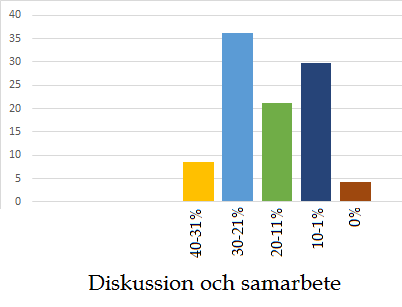
\includegraphics{Figures/Barcharts/diskussion.png}
    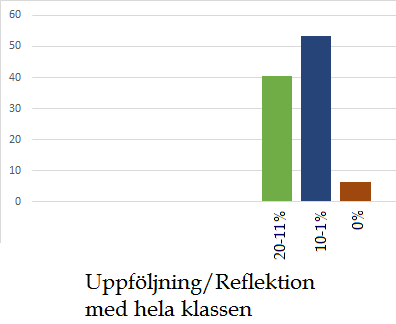
\includegraphics{Figures/Barcharts/uppfoljning.png}
    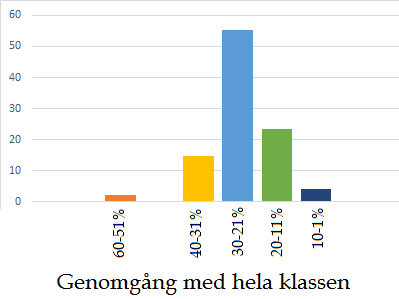
\includegraphics{Figures/Barcharts/genomgang.png}
    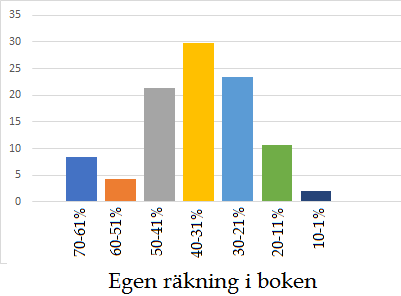
\includegraphics{Figures/Barcharts/rankning.png}
    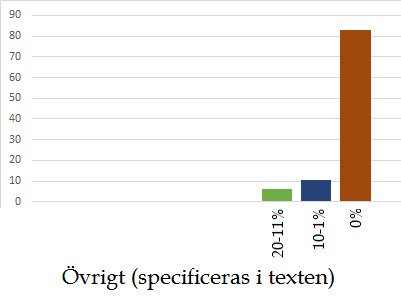
\includegraphics{Figures/Barcharts/ovrigt.png}
    \caption{Figurerna visar stapeldiagram som representerar hur stor andel av lektionstiden som olika lärarna anger att de lägger på olika delar av undervisningen. På y-axeln representeras mängden svar i procent, och på x-axeln uppskattad tid lagd på de olika momenten. Notera att y-axeln växlar skala mellan de olika diagrammen.} %I figur (a)-(e) visas cirkeldiagram som visar hur stor andel av lektionstiden som olika lärare anger att de lägger på olika delar av undervisningen. Figur (f) visar det intervall (i procent) som varje färg representerar.}
    \label{fig:PC}
\end{figure}

    \textcolor{lila}{Genom att studera stapeldiagrammen i figur~\ref{fig:PC} kan man notera att den största delen av lektionstiden används till genomgång och egen räkning. Därefter följer elevdiskussion och uppföljning, och utöver detta lägger en liten andel av lärarna även tid på andra saker. Under övrigt faller framförallt laborationer, spel, digitala quiz, redovisningar framförda av eleverna samt problemlösning.}

    \textcolor{lila}{Några av lärarna kommenterade också i samband med den här frågan att de uppmuntrar eleverna att jobba tillsammans med uppgifterna i boken, och att det på så sätt blir mindre individuellt arbete, och mer diskussion mellan eleverna.}

\subsubsection{Vad är problemlösning för dig?}
    \textcolor{lila}{Här bad vi lärarna att skriva en kort förklarande text om hur de definierar problemlösning. I de svar vi fick in kunde vi hitta några olika karatäriserande åsikter, och undersöka hur stor andel av lärarna som nämner de olika delarna.}

    \textcolor{lila}{Många lyfte fram att ett problem är \textsl{en uppgift som man på förhand inte vet hur man ska lösa, och där man får applicera känd kunskap på nya situationer}. Detta är den vanligaste definitionen, och även den vi enligt avsnitt~\ref{sec:problemdef} använder i denna rapport. Hela $79\%$ hade med detta som ett kriterium i sina definitioner av problemlösning.}
    \textcolor{lila}{En annan viktig faktor, som nämndes av ungefär $20\%$, var \textsl{öppna problem}. Dessa definieras i avsnitt~\ref{sec:problemdef}. som problem som går att lösa på flera olika sätt, och i vissa fall även kan ge olika svar. Ett exempel på ett öppet problem är att man ska planera en pool med en viss volym, vilket självklart kan göras på en mängd olika sätt.}

    \textcolor{lila}{Därefter följde två kriterier, som vardera nämndes av cirka $16\%$. Det ena var att problemlösning \textsl{ska utgå från en större uppgift, vilket man måste använda flera olika metoder för att lösa}. Den andra pekar på att ett problem \textsl{innehåller antingen för mycket eller för lite information}. Det innebär att man antingen måste sortera ut det man behöver eller finna ytterligare information Detta kan göras genom att hitta denna via någon källa eller genom egna uppskattningar.}

    \textcolor{lila}{Ungefär $5\%$ av lärarna nämnde att problemlösning bör genomföras \textsl{i par eller grupper} och att det handlar om \textsl{diskussion och reflektion}. Lika många angav att det inkluderar att använda sig av \textsl{modellering}, att man får \textsl{tillämpa matematik} eller att problemlösningsuppgifter har en \textsl{verklighetsanknytning}. En liten andel poängterade att problemlösning ofta innebär att man \textsl{måste prova sig fram för att hitta en korrekt lösningsmetod} och cirka $7\%$ tog upp att problemlösningsuppgifter ofta utgår från en \textsl{textuppgift}. En lärare svarade även enbart med ordet ''Textuppgifter''.}

\subsubsection{Mer problemlösning i matematiken}
\label{sec:MerProblemlosning}

\textcolor{lila}{Hela $91\%$ anger att de arbetar för att inkludera problemlösning i sin undervisning. Detta motiveras till viss del med att det ingår i kursplanen, vilket $19\%$ av lärarna nämner i sin motivering. Men utöver det skriver även hela $81\%$ av lärarna att de gör det för att de tycker att det är viktigt med problemlösning. De poängterar att det är en stor del av matematiken, och att det är bra att kunna angripa problem man inte tidigare stött på i många sammanhang, även inför framtiden på arbetet eller universitetet. De $9\%$ som angav att de inte arbetade med problemlösning angav tidsbrist som en motverkande faktor. Det är mycket som behöver gås igenom, och då man ofta kan klara nationella provet utan problemlösning prioriteras detta ner. Någon sa också att det berodde på att de inte visste hur man skulle göra det på ett bra sätt, och att det är svårt att gå ifrån den undervisningsmetod man är van vid.}

\textcolor{lila}{När vi bad alla lärare att fundera på vad det finns för svårigheter med att införa mer problemlösning, fick vi många intressanta infallsvinklar. Av de som svarade nämnde $42\%$ att de tyckte att det är \textsl{svårt att hitta bra problem}. Ett bra problem ska ju vara utmanande för hela klassen, och då det ofta finns en mycket stor spridning i matematikkunskaperna hos en klass är detta inte helt lätt. Det tar också \textsl{tid}, och det nämns också som en stor bidragande faktor till varför man inte har mer problemlösning än vad man har, och nämns av $38\%$ av de svarande lärarna. Att elevernas tidigare skolår präglats till stor del av traditionell undervisning är också del av problematiken. $29\%$ av lärarna tar upp att eleverna ofta har för dåliga förkunskaper för att kunna ta sig an större problemuppgifter, samt att de också ofta är skeptiska till annan form av matematik än den de  är vana vid. Detta anges gälla speciellt för de högpresterande eleverna. En liten andel anger också att det som lärare kan vara svårt att ändra sin undervisning, och lätt att ''falla tillbaka i gamla hjulspår''.}

\textcolor{lila}{Trots dessa svårigheter är det ändå som sagt $91\%$ av lärarna som arbetar med att införa mer problemlösning i sin undervisning. Varför jobbar man så hårt med detta? Lärarna fick frågan om vad de ser för möjligheter med problemlösning. Många framhäver här att det är väldigt nyttigt att lära sig att \textsl{tänka på nya sätt}, och att även \textsl{lyfta styrkorna i olika tankesätt}. Det är också viktigt att kunna \textsl{hitta relevant information} vid ett givet problem, och detta är färdigheter som kan appliceras i många fler sammanhang än bara vid skolbänken. Mer problemlösning nämns också som ett bra sätt att få \textsl{tillämpa} sin kunskap, och därmed få se hur matematikens många delar kan användas i verkligheten, vilket ger en \textsl{relevans} till ämnet. Det är också ett bra sätt för eleverna att träna på att \textsl{samarbeta} samt att få \textsl{diskutera} matematik, samt att det \textsl{går att anpassa till olika nivåer}. Rätt uppgift kan vara ett problem för en hel klass, och ger alla en chans att \textsl{utgå från liknande villkor}.}
    
    
    \subsection{Intervju med Niklas Grip}
    %Vem är Niklas
\textcolor{turkos}{
För att få ett perspektiv ifrån någon som faktiskt undervisar i matematik och höra den personens åsikter om problemlösning kontaktade vi Niklas Grip. Niklas är ämneslärare i matematik på Mikael Elias teoretiska gymnasium i Göteborg och har bland annat kursen Matematik – specialisering som han inriktat mot just problemlösning.
}

% Hur genomfördes intervjun, samt våra frågor till honom. 
\textcolor{turkos}{
Intervjun genomfördes som ett djupgående samtal mellan oss och Niklas, där Niklas gavs stort utrymme att svara fritt. Samtalet var uppstyrt kring följande fyra frågor, samt följdfrågor på dessa: 
}
\begin{itemize}
  \item \textcolor{turkos}{Arbetar du med problemlösning i din undervisning?}
  \item \textcolor{turkos}{Hur definierar du problemlösning?}
  \item \textcolor{turkos}{Kan du ge några exempel på problem du använt i din undervisning?}
  \item \textcolor{turkos}{Hur arbetar du med teknik i din matematikundervisning?}
\end{itemize}

\noindent \textcolor{turkos}{
Följande är sammanfattning utav intervjun där vi försöker komprimera det det viktigaste som Niklas sa. De citat som tas upp kommer beskriva det som vi tyckte var av särskilt intresse eller vikt under intervjun. 
}

\subsubsection{Niklas syn på problemlösning}

% Hur undervisar han problemlösning? och %Exempel på problem han har använt. 
\textcolor{turkos}{
Niklas arbetar med problemlösning på flera olika sätt. Dels så använder han problemlösning som en metod för att introducera nya begrepp för sina elever, men han har även lektioner helt inriktade på problemlösning och öppna frågeställningar. Han berättar att han inte får in lika mycket öppna problem som han skulle önska. Som ett exempel på vad ett öppet problem är tar Niklas upp att han bett sina elever räkna ut hur stor sannolikheten är att bli träffad utav en fågelskit under ett liv. Andra problem han jobbar med är klassiska optimeringsproblem, så som att dra en kabel över en flod. Till sist så har han hand om gymnasiearbeten som inriktar sig mot problemlösning, några av hans elever räknade ut vilken ''starter pokémon'' som var bäst i ett pokémonspel. Själv tycker han att han lyckas få in hela skalan av problemlösning i sin undervisning.
}

%Problem med problemlösning?
\textcolor{turkos}{
Niklas ser tre svårigheter med sitt arbete med problemlösning. Den första är att han har många högpresterande elever som har en väldigt klar bild utav vad matematik är och som ofta blir negativt inställda till lektioner som går utanför deras bild av vad en matematiklektion ska innehålla. Den andra är att de nationella proven i framför allt matematik 2 till 4 inte testar problemlösning, vilket leder till att både Niklas och hans elever tappar lite av motivationen att jobba med problemlösning.}

\textcolor{turkos}{Den tredje svårigheten som Niklas nämner är det rent pedagogiska i hur man ska undervisa om problemlösning. Niklas upplever att överallt så talas det gott om problemlösning, men att det finns lite hjälp att få ifrån andra lärare eller andra personer när det gäller saker som hur man ska göra när en elev fastnar i ett problem. Han efterfrågar en undervisningskultur runt problemlösning där han kan diskutera sina erfarenheter och svårigheter med andra lärare: 
}

% Indrag på marginalerna, mindre text. Inget citattecken, beskriv i texten. Skriv efteråt hur vi tolkar det. 
\begin{displayquote}
\textcolor{turkos}{Det är väl kanske de här sakerna som jag sa förut att det finns en lite väldigt svag kultur och med det också goda exempel på hur man undervisar om just själva problemlösande. Det finns både forskning och litteratur om det, och det har funnits länge.}
\end{displayquote}

\noindent\textcolor{turkos}{
Niklas upplever alltså att trots tillgång till mycket resurser så känner han att hans arbete med problemlösning bedrivs mycket på egen hand. När det gäller undervisning utav andra delar av matematiken så har han hjälp utav böcker, andra lärare och YouTube-kanaler som visar hur man löser uppgifter. Han upplever däremot att det är väldigt få som inriktar sig på den generella förmågan att lösa problem. Niklas tar upp att han försökt lära sina elever att arbeta enligt Pólyas metoder (se \ref{sec:polya}). Han känner dock att han misslyckas få dem att förstå dem och inse vad som är relevant med dem, där hade andra lärares tankar kunnat vara till stor hjälp för honom.
}

%Hur definerar han problemlösning?
\textcolor{turkos}{
Niklas definierar själv problemlösning väldigt brett, för honom kan allt vara problemlösning. Huruvida en uppgift är ett problem eller ej beror på kunskapen hos personen som försöker lösa det:
}

\begin{displayquote}
\textcolor{turkos}{
Kommer man till problem som man inte riktigt vet hur man ska lösa så upplever jag att det är då man använder sin problemlösningsförmåga.
}
\end{displayquote}

\textcolor{turkos}{
Det är viktigt att man förstår var elevernas kunskap ligger. Niklas berättade att han ibland har haft lärarpraktikanter som varit med på hans lektioner där han använt problemlösning som en metod för att lära sina elever hur de ska använda enhetscirkeln. Praktikanterna förstod inte hur det kunde vara problemlösning när Niklas hade haft genomgång om enhetscirkeln dagen innan, men i och med att eleven själv fick ta reda på hur de skulle använda sig av den så blev det ändå problemlösning i slutändan. 
%Det är den idéen som Niklas använder som grund när han använder problemlösning för att introducera nya begrepp. Kan en elev inte lösa andragradsekvationer så det utmärkt tillfälle att både lära sig ett nytt begrepp och öva upp sin problemlösningsförmåga. 
}

%Hur jobbar han med teknik och tekniska hjälpmedel
\textcolor{turkos}{
Niklas har introducerat sina elever till Geogebra, kalkylark och programmering, och han ser hur verktygen hjälper eleverna att förstå vad olika uppgifter handlar om. Han förklarar att elever som använder sig utav Geogebra kommer kunna kontrollera sina lösningar X sätt än vad elever som löser uppgiften med enbart algebra kommer att kunna göra. Niklas trycker på att det han vill är att eleverna själva ska använda sig av verktygen utan att han behöver visa dem hur de ska göra. Det är när eleverna själva får sitta med verktygen som de verkligen börjar lära sig teknikerna.
} 

%\subsubsection{Niklas kommentarer på våra problem}
    \label{sec:intervju}
    
\section{Skapande av problembank med tillhörande problem}
    \label{sec:skapandetavproblembank}
    \textcolor{lila}{Här presenteras processen bakom hur problemen konstruerades och vilka tankar som låg bakom. Även utvecklingen av webbplatsen samt de metoder som användes där förklaras mer ingående.}
    
    \subsection{Konstruktion av matematiska problem}
    \label{sec:Skapandetavproblem}
        \textcolor{lila}{De problem som har skapats har som tidigare nämnts konstruerats med målet att öka andelen problemlösning i gymnasiet. För att uppnå detta har vi vid skapandet av problemen utgått från ett antal riktlinjer, där en eller flera av dessa belyses i varje problem.}

\textcolor{lila}{Den första, och kanske viktigaste, riktlinjen är att problemen ska leda till ett \textsl{undersökande arbetssätt}, se avsnitt~\ref{sec:problemdef}. I samma avsnitt diskuteras även \textsl{öppna problem}, som också var en bakomliggande tanke för många av problemen. Vi har även skapat problemen med avsikt att träna eleverna på \textsl{modellering} och \textsl{programmering}, vilka tas upp i avsnitt \ref{sec:problemdef} respektive \ref{sec:ProgrammeringOchMatematik}. \textsl{Verklighetsanknytning} ska också enligt avsnitt~\ref{sec:Verklighetsanknytning} finnas med i flera av problemen. Alla problemen har också konstruerats för att vara \textsl{rika problem}, se avsnitt~\ref{sec:Diskussion} som kan leda till en givande diskussion.}

\textcolor{lila}{Med detta som underlag har vi skapat olika problem. Vi har tagit inspiration från våra egna erfarenheter från hela vår skolgång, inklusive universitetet, samt från en mängd olika böcker, som nämns i samband med respektive problem. Utifrån vår grundidé har vi därefter arbetat oss vidare för att skapa ett problem som passar gymnasieelever. På så sätt har vi tagit fram problem som alla har tre gemensamma delar: \textsl{Introduktion}, \textsl{Genomförande} och \textsl{Diskussion}.}

\textcolor{lila}{I introduktionen presenteras problemet, och i vissa fall ingår där ett antal frågor att diskutera innan man börjar räkna på problemet. Själva problemet genomförs i grupper om två, och därefter kommer diskussionen. Denna börjar i vissa fall med att man går ihop i lite större grupper och presenterar och diskuterar sina lösningar av problemet, förklara varför man gjort som man gjort och jämföra eventuella olika lösningsgångar. Avslutningsvis diskuterar klassen problemet tillsammans, eventuellt med hjälp av våra föreslagna diskussionsfrågor. Vikten av att diskutera  problemet ordentligt presenteras i avsnitt~\ref{sec:Diskussion}.} 

\textcolor{lila}{Till varje problem följer också \textsl{Information till läraren}, med information om problemets mål samt eventuella förkunskaper och material som behövs. Det finns också \textsl{Ytterligare information}. Dit kan höra förslag på hur problemet kan introduceras, bakgrundsinformation som kan vara bra för läraren att repetera innan problemet genomförs med klassen samt tankar om vilka frågor som skulle kunna dyka upp vid diskussionerna och hur dessa kan hanteras. Till många problem finns också en presentation, som läraren kan välja att använda. På så sätt presenteras problemen tillsammans med en komplett lektionsplanering.}

\textcolor{lila}{Vi har även skrivit en text som förklarar tanken med våra problem. Där presenteras upplägget samt några idéer på hur man ska agera som lärare, bland annat genom att undvika att framställa ett förslag som felaktigt.}

\textcolor{lila}{De problem som ska testas har planerats för att ta ungefär 50 minuter att genomföra. Detta för att de ska kunna genomföras under en lektion på en timme, och att det ska finnas tid över att svara på utvärderingsenkäten, vilken kommer att diskuteras i kapitel~\ref{sec:testavproblemen}.}

\textcolor{Mahogany}{Metoden kring hur vi utformade problemen och vilken nivå de skulle ligga på var att vi med relativt stor frihet tog fram problem på gymnasienivå.
Den mer specifika nivån var menad att vara anpassningsbar, på det sättet att man med hjälp av fördjupningsfrågor kunde fördjupa sig inom ämnet och därmed kunna försvåra problemet om så önskas.
I det senare stadiet av projektet blev det dock viktigare att bestämma en nivå då lärare som skulle testa problemen ofta enbart undervisade på en specifik nivå. Behovet av att bestämma en nivå för problemen, alternativt anpassa problem utefter en viss nivå, blev därmed större.}

    \subsection{Utvecklingen av webbplatsen}
        \textcolor{green}{Webbplatsen utvecklades i skriptspråket Javascript. Fördelarna med detta jämfört med till exempel använda HTML är att man kan designa sidan på många fler sätt och få total kontroll över sidans innehåll. Med total kontroll menas det att man skulle kunna ha annat material på webbplatsen än bara text- och bildmaterial. Det skulle kunna vara någon form av digitalt verktyg, till exempel ett matematiskt problem som använder sig av en simulator. Detta kan göras med hjälp av Javascripts många olika bibliotek.}

\textcolor{green}{Biblioteket som användes för att utveckla webbplatsen var React JS. React JS är ett av de mest populära biblioteken att bygga webbplatser med i Javascript [källa]. I Reacts bibliotek finns främst verktyg för att jobba med vy-delen av en hemsida, det vill säga det visuella som besökaren ser. Vill man integrera tyngre applikationer i webbsidan så finns möjligheter för det. Men om vyn är det största fokuset så är React ett mycket lämpligt val då det är väldokumenterat och gör det enkelt att bygga vidare på hemsidans design. Detta är till stor del baserat på våra tidigare erfarenheter och personliga preferenser inom webbutveckling.}
        
\section{De slutgiltiga problemen}
    %"Resultat": Webbplatsen och alla problemen
        %\textcolor{lila}{Det färdiga resultatet presenteras i form av en webbplats med de skapade problemen samt tillhörande information.} 
    
    %\subsection{De problem som vi skapat}
        \textcolor{lila}{Här presenteras huvuddragen av varje problem samt den tillhörande informationen. Notera att allt runtomkring själva problemet enbart är förslag, och att varje lärare kan anpassa genomförandet efter hur hen tror att det blir bäst i en specifik klass. Problemen i avsnitt \ref{sec:Fermi} till och med \ref{sec:Sortera} är allmänna problem som inte kräver några speciella förkunskaper från läraren, förutom det som skickas med som kompletterande information. Övriga problem baseras på programmering, och det är då lättare för läraren att hjälpa till med koden om denne kan programmera. Notera dock att det är problemlösningen som står i centrum, och inte kodens specifika syntax. Lärarna får även själva välja vilket programmeringsspråk som ska användas, men som vägledning skickas ett lösningsförslag skrivet i Java. Alla problemen finns även i sin fullständiga form i appendix~\ref{appendix:Problem}.}

\subsubsection{Fermiproblem}
    \label{sec:Fermi}
 
    \textcolor{lila}{Målet med detta problem är att eleverna ska få träna på att göra uppskattningar, samt att bryta ner ett problem i mindre delar.}
    
    \textcolor{lila}{Som inledning presenteras vad ett \textsl{fermiproblem} är. Det innebär att man, i fall där ett specifikt värde är svårt alternativt omöjligt att mäta, bryter ner problemet i många små delar och uppskattar varje del för sig. På så sätt kan man uppskatta lösningen på frågor som vid första anblick kan verka omöjliga. För att illustrera detta visas även ett exempel på ett fermiproblem, samt exempel på hur man kan dela upp det i minde delar.}

    \textcolor{lila}{Eleverna får en lista med olika fermiproblem att välja mellan, och ska arbeta i grupper om 2. Först ska de gissa på svaret, och sedan beräkna det genom att dela upp i delar som man kan uppskatta. Därefter får de i mindre grupper presentera och diskutera sitt arbete. Slutligen diskuteras i helklass om resultaten kändes rimliga, hur genomförandet gick, ifall lösningsmetoden är användbar samt varför den fungerar så bra som den gör. För den sista frågan ger vi även lärararen svaret, det vill säga att det fungerar eftersom man ibland överskattar och ibland underskattar de mindre delarna, vilket gör att det slutgiltiga resultatet ofta blir en mycket bra uppskattning.}

\subsubsection{Flygplan}
    \label{sec:Flygplan}
    
    \textcolor{lila}{Detta  problem syftar till att träna eleverna på ett undersökande arbetssätt där inte alla påverkande faktorer är givna, utan måste resoneras fram av eleverna. Den leder också fram till ett ekvationssystem, vilket ger ett exempel på när dessa är användbara.}
    
    \textcolor{lila}{En Sverigekarta med utmarkerade flygplatser och flygrutter presenteras för klassen, se figur~\ref{fig:Flygplan}. Detta görs bitvis, med plats för en kort diskussion om vad frågeställningen skulle kunna vara, givet den dittills givna informationen. Med all information given får eleverna i grupper om två arbeta med en specifik sträcka, Visby-Karlstad. På vilka olika sätt kan man ta sig mellan dessa två städer? Vilken sträcka är bäst och vilka faktorer påverkar detta? Därefter specificeras uppgiften ytterligare, genom att de får reda på hur mycket det kostar att åka mellan två olika direkta flygsträckor. De ska nu hitta den \textsl{billigaste} vägen mellan Karlstad och Visby, samt vilken väg som blir billigast om man ska från Karlstad till Stockholm, men sträckan Stockholm-Göteborg är fullbokad. Den avslutande helklassdiskussionen tar bland annat upp vilka faktorer som påverkar bränslekostnaden, vilka faktorer som påverkar biljettpris för en specifik sträcka och ifall det är det totala avståndet eller antalet mellanlandningar som avgör priset för en resa.}
    
    \textcolor{lila}{Under punkten ''Ytterligare information'' diskuteras tankar bakom uppgift och diskussion. Eleverna får själva upptäcka att priset beror på sträckan, men att det också tillkommer ett fast pris för start och landning, vilket speciellt visar sig i att det för sträckan Karlstad-Göteborg blir billigare att flyga en längre sträcka, men med färre mellanlandningar. De får också själva reflektera över ytterligare faktorer som skulle kunna påverka priset, till exempel löner och vinstmarginal.}
    
\subsubsection{Fritt fall}
    \label{sec:FrittFall}
    
    \textcolor{lila}{Tanken med problemet är att eleverna ska få använda derivata utifrån en verklig situation istället för utifrån en färdig formel, samt få en djupare förståelse för vad derivata egentligen är.} 
        
\begin{figure}
    %\centering
    \hspace{0.4cm}
    \begin{subfigure}[b]{0.45\textwidth}
        \centering
        %\hspace{-40pt}
        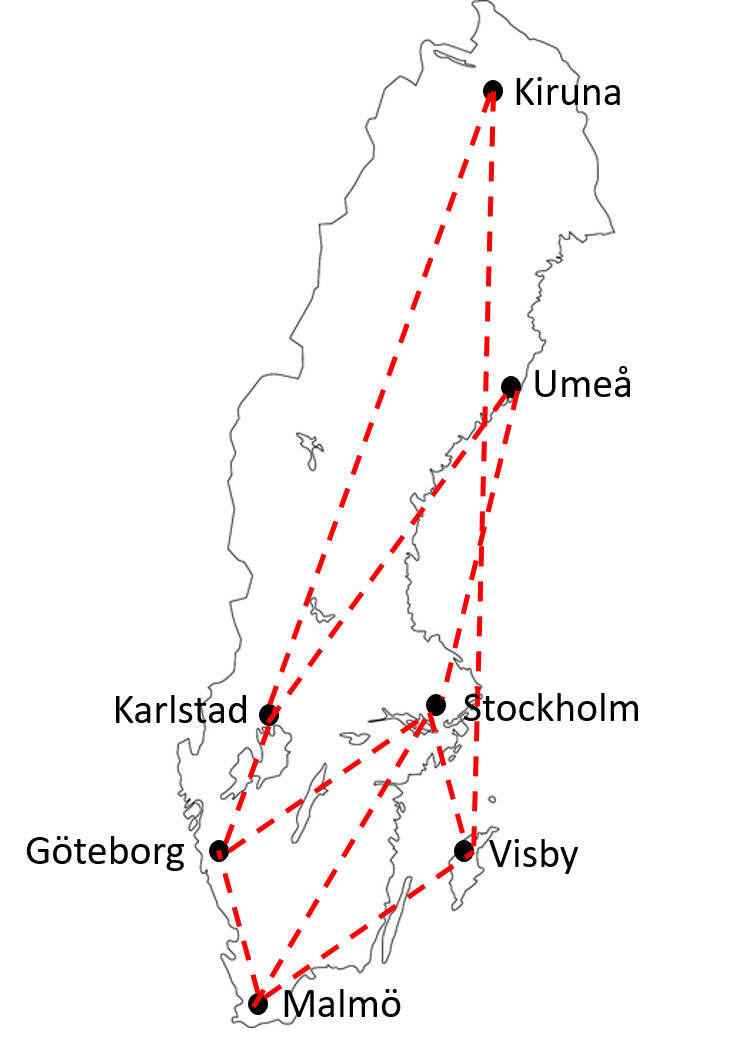
\includegraphics[width=0.9\textwidth]{Figures/Flygplan_rapport.png}
        \caption{\textsl{Sverigekarta med utmarkerade flygplatser och rutter.}}
        \label{fig:Flygplan}
    \end{subfigure}
    \hfill
    \begin{subfigure}[b]{0.45\textwidth}
        \centering
        %\hspace{-40pt}
        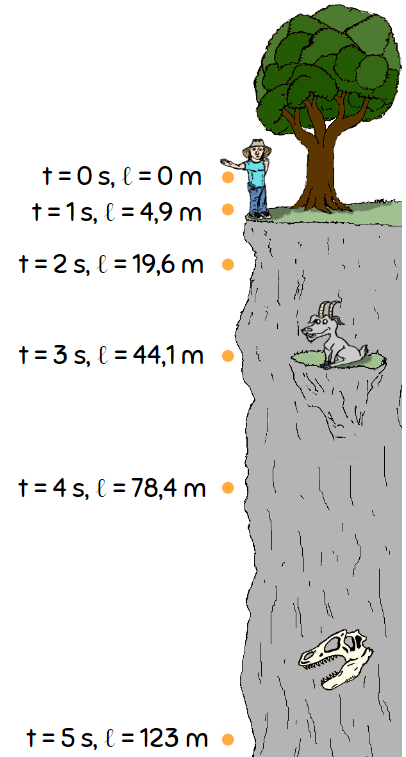
\includegraphics[width=0.7\textwidth]{Figures/FrittFall.PNG}
        \caption{\textsl{Fallande boll med angivna fallsträckor för varje sekund.}}
        \label{fig:FrittFall}
    \end{subfigure}
    \hspace{0.4cm}
    \caption{Figurer tillhörande två av problemen, ''Flygplan'' till vänster och ''Fritt fall'' till höger.}
    \label{fig:three graphs}
\end{figure}
    
    \textcolor{lila}{Som en introduktion till problemet diskuterar man tillsammans i klassen vad en derivata är och hur man kan beräkna den. Därefter presenteras en bild av en fallande boll, med utmarkerade fallsträckor för olika tider, se figur~\ref{fig:FrittFall}. Frågan är nu vad man utifrån detta kan komma fram till om bollens hastighet och acceleration, vilket klassen får arbeta med i grupper om två. Tanken är att man ska konstruera en graf över sträcka som en funktion av tid, och utifrån denna använda en linjal för att rita tangenter längs med grafen och därmed skapa en graf över hastighet som en funktion av tiden. Därefter kan samma procedur genomföras för att rita accelerationen som funktion av tiden. Denna bör, med avvikningar på grund av felkällor, bli konstant och ungefär lika med tyngdaccelerationen, det vill säga ungefär~10. Avslutningsvis diskuteras denna metod med avseende på resultat och noggrannhet.}
    
\subsubsection{Försvåring av en ekvation}
    \label{sec:ekvation}

    \textcolor{lila}{Detta är en mycket fri uppgift med målet att ge eleverna en djupare förståelse för ekvationer och ekvationslösning.}

    \textcolor{lila}{Inledningsvis diskuteras begreppet ekvation, samt hur man löser en ekvation, i helklass. Det viktiga här är att komma fram till att så länge man gör samma sak på båda sidorna om likhetstecknet, och använder prioriteringsreglerna rätt, så får man göra vad som helst. Eleverna får därför två och två arbeta med att ''försvåra'' ekvationen x=2, genom att i flera steg göra en bestämd operation i både vänster- och högerledet. Följande enkla exempel på hur man kan börja presenteras för eleverna som tips på hur man kan börja}
    
        \begin{equation*}
            x=2
        \end{equation*}
        \begin{equation*}
            2x=4 \quad (\cdot2=\cdot2)
        \end{equation*}
        \begin{equation*}
            2x+5=7+2 \quad (+5=+3+2)
        \end{equation*}
    
    \noindent\textcolor{lila}{Varje steg ska även skrivas upp och motiveras enligt ovan. Därefter diskuteras lösningsgången, samt potentiella utvecklingar. Eleverna får också diskutera ifall det finns någon lösning på ekvationen, och hur den i så fall ser ut. De får på så sätt reflektera över att de nu har ''löst en ekvation baklänges'' och att varje ekvation, som kan tyckas se jobbig ut, kan brytas ner i små, enkla steg.}

\subsubsection{Matematisk modell för bil och löpare}
    \label{sec:lopare}
    
    \textcolor{lila}{Detta problem är ursprungligen förklätt som en enklare standarduppgift, men låter därefter eleverna fundera över den matematiska modell de har använt, samt ifall den är rimlig. Målet är att visa fördelar och nackdelar med matematiska modeller, samt införa ett sunt kritiskt tänkande hos eleverna.}
    
    \textcolor{lila}{Inledningsvis får eleverna i par lösa två till synes likartade uppgifter av standardkaraktär. I den ena får de givet hur snabbt det tar att köra en viss sträcka med bil, och ska beräkna hur lång tid ett antal andra sträckor tar att köra. I den andra uppgiften är bilen utbytt mot en löpare, men för övrigt är det samma frågeställning. Vi upplyser här läraren om att vi antar att de flesta elever kommer använda en linjär modell, dvs anta att både bilen och löparen håller samma fart oavsett sträcka. Därefter diskuterar men resultaten i helklass, samt vilka antaganden man har gjort, om de är rimliga och om det skiljer sig mellan bilen och löparen. Som jämförelse får man reda på att den tid som med den linjära modellen fås för den längsta sträckan för löparen är betydligt snabbare än världsrekordet, och man får även verkliga tider för de efterfrågade sträckorna\footnote{Tiderna för löparen som använts är tagna från hur fort Axel, medförfattare i detta arbete, springer dessa sträckor.}. Utifrån detta får eleverna diskutera vilka faktorer som avgör, till exempel att man orkar springa snabbare på kortare sträckor, men också att startsträckan tar upp större delen av tiden.}
    
\subsubsection{Sortera en kortlek}
    \label{sec:Sortera}
    
    \textcolor{WildStrawberry}{
        Kortleken är ett enkelt sätt för en elev att få en god introduktion till hur enkla sorteringsalgoritmer fungerar samt hur man nyttjar sig av dem.}
        
    \textcolor{WildStrawberry}{
        Lektionen kommer innefatta att eleven får en introducerande beskrivning på vad en algoritm är och hur den kan användas. Sedan kommer eleverna få fundera en stund på hur man kan utnyttja algoritmer till att bryta ner större problem till enkla upprepande arbetsflöden. Till uppgiften så kommer kortlekar att tillhandahållas till eleverna som får instruktioner på hur man får interagera med sina kort när man försöker sortera dem. Dessa instruktioner efterliknar sättet en dator jämför och byter position på element i en lista. När eleverna fått experimentera och kommit fram till sina algoritmförslag så skriver de ner sina instruktioner. De byter instruktioner med en annan grupp och ska kunna sortera sina lekar genom att enbart följa instruktionerna, precis som en dator hade gjort. }
        
    \textcolor{WildStrawberry}{
        Den stora lärdomen i denna uppgift är att eleverna i fråga troligtvis lyckas skapa algoritmer som har givna namn och som faktiskt används i ''den riktiga världen''.  Eleverna kommer få reflektera över vad som gått bra, eller dåligt, och hur man kan göra optimeringar eller fixa problemen (''buggarna'') som uppstod. Ungefär som en riktig programmerare får göra. \todo{:)}}
        
\subsubsection{Approximera ett irrationellt tal}
    \label{sec:approx}

\subsubsection{Binär till decimal}
    \label{sec:binar}
    
\subsubsection{Fibonaccis talsekvens}
    \label{sec:Fibonacci}
    
    \textcolor{WildStrawberry}{
        Fibonaccis talsekvens är mycket klassiskt problem när det kommer till programmering. Det är ofta en startpunkt för rutinerade programmerare som försöker lära sig syntaxen i nya programmeringsspråk (förutsatt att man känner till lösningen). }
        
    \textcolor{WildStrawberry}{
        Undervisningen börjar med att läraren introducerar Fibonaccis talsekvens och hur talföljden utvecklar sig. Efter detta kommer eleverna försöka skapa egna stycken kod som ska skriva ut talföljden. Mer erfarna programmerare uppmuntras till att prova lösa uppgiften med hjälp av rekursion. När väl eleverna provat att lösa uppgiften så kommer en diskussionstund där man bör reflektera på hur det har gått, hur väl sin kod fungerar och vilka optimeringar som man kan göra. Slutligen kan man diskutera och reflektera över hur man kan använda sig av loopar för att lösa problem.}
        
    \textcolor{WildStrawberry}{
        I denna uppgift får får eleven träning i iterativa och rekursiva loopar. Båda vilka är verktyg som programmerare behöver kunna använda sig utav. Lär man sig behärska dessa tekniker så kommer man i sin följd kunna lösa andra problem som har iterativ, eller rekursiv, struktur.}
        
\subsubsection{Identifiera primtalsfaktorer}
    \label{sec:primtal}

\subsubsection{Personnummer}
    \label{sec:Pnr}
    
    \textcolor{WildStrawberry}{
        slack}
        
\subsubsection{Primtalsfaktorer}
    \label{sec:Primtal}
    
    \textcolor{WildStrawberry}{
        Att kunna faktorera tal in till primtal är något man kan råka stöta på i sitt liv. Kanske speciellt om man någon gång behöver nyttja sig av eulers phi-sats..... \todo{this is bajs!} }
        
    \textcolor{WildStrawberry}{
        För att introducera detta problem så krävs ingen lång bakgrund, så exempelvis kan läraren skriva upp en mängd siffror som elevernas program ska kunna köra. Sen kommer eleverna, i små grupper om 2 eller 3, försöka skapa program som hanterar alla fallen. Slutligen kommer klassen diskutera hur man hanterat fallen där talen haft fler än 2 primtalsfaktorer, upprepande faktorer och vilka ''fel'' man kan fånga med sina program. }
        
    \textcolor{WildStrawberry}{
        Under detta tillfälle så kommer eleven få öva på enkla booleanska uttryck, matematiska operatorer, optimering av kod och eventuella fält eller listor. Det blir en salig blandning av olika moment i programmering och man utsätts för många olika syntax i en och samma uppgift.}

\subsubsection{Skapa ett chiffer}
    \label{sec:chiffer}
    
\subsubsection{Sorteringsalgoritmer}
    \label{sec:sorteringsalgoritmer}
    
\section{Webbplatsens slutgiltiga upplägg}
    \textcolor{Mahogany}{Webbsidan består framför allt av olika problem som med hjälp av titel samt varsin tillhörande ikon listas i ett rutnät på ''Problem''-sidan. Klickar man på ett av problemen så kommer man vidare till en mer detaljerad vy med en kort beskrivande text följt av en länk till det fullständiga problemet. I många fall bifogas även en tillhörande PowerPoint, som är tänkt att underlätta utförandet.}

\textcolor{Mahogany}{Hemsidan har även en startsida där besökaren ges en introducerande text om vad vi arbetar med samt att man via ett enkelt knapptryck lätt tar sig vidare till problemen. Dessa kommer man givetvis också åt via menyn, skillnaden är att vi vill fånga uppmärksamheten på ett mer välkomnande sätt för den som besöker hemsidan för första gången genom att ha en knapp över en bild som illustrerar några av våra problem.}

\textcolor{Mahogany}{Till sist så inkluderas sidan ''Om oss'', som beskriver projektets arbete, samt en sida med ''Information till läraren'', vars innehåll beskrivs närmare i \ref{sec:Skapandetavproblem}.}
    
\section{Test av problemen}
    \label{sec:testavproblemen}
    \textcolor{Mahogany}{Det här kapitlet behandlar de testresultat som mottogs från utvärderingsenkäten för de lärare som testat ett eller flera av de framtagna problemen. Inledningsvis förklaras testmetoden och därefter följer testresultaten. Här sammanfattas även några av de resultat som ansågs vara viktigast och efter det beskrivs varje testat problem i detalj. Avslutningsvis presenteras elevernas egna definitioner av begreppet problemlösning.}
    
    \subsection{Hur testet genomfördes}
        \label{sec:HurTestetGjordes}
        \textcolor{lila}{Av de 58 lärare som svarade på utvärderingsenkätetn som presenterades i avsnitt~\ref{sec:Bakgrunsenkat} var det 20 stycken som fyllde i ett intresse för att testa ett av våra problem.} 

\textcolor{lila}{De sex problem som presenterades i avsnitt \ref{sec:Fermi} till och med \ref{sec:Sortera} fördelades mellan dessa, där hänsyn även togs till vilka kurser lärarna hade angivit att de för tillfället undervisade i. Problemen skickades ut fredagen den 31:e mars, tillsammans med dokumentet "Allmän information till lärare" samt tillhörande presentation. Därefter fick lärarna 5 veckor på sig att genomföra problemen, det vill säga till den 5:e april.} 

\textcolor{lila}{Lärarna hade som tidigare nämnt möjlighet att följa det givna upplägget till den grad de själva ville, och därefter fick de en utvärderingsenkät. Den innehöll frågor om hur de tyckte att problemet presenterats från vårt håll, om de valt att ändra något eller om det var något annat de saknade samt om hur de tyckte att problemet togs emot av eleverna. Eleverna fick en liknande utvärderingsenkät där de fick skriva sin definition av problemlösning, vad de tyckte om problemet, vad de tyckte om nivån på problemet samt om de upplevde att de lärt sig något.}

        
    \subsection{Vad testet visade}
    \label{sec:slutenkat}
    \textcolor{lila}{Nedan presenteras svaren på de utvärderingsenkäter vi fick in. De uppgifter som testades var ''Fermiproblem'', ''Försvåring av ekvation'' och ''Matematisk modell för bil och löpare'', vilka förklaras närmare i avsnitt~\ref{sec:Fermi}, \ref{sec:ekvation} respektive \ref{sec:lopare}. Niklas grip, som presenterades i avsnitt~\ref{sec:intervju} i samband med den intervju han medverkade i, testade också några av programmeringsproblemen, det vill säga problem~\ref{sec:sorteringsalgoritmer} till och med \ref{sec:chiffer}. Först presenteras de viktigaste resultaten av undersökningen, och därefter följer varje problem för sig, med svar från lärare och i de flesta fall elever. Sist följer elevernas svar på frågan ''Vad är problemlösning för dig?''.}

    \subsubsection{Sammanfattning av några av de viktigaste resultaten}
    \textcolor{lila}{Sammanfattningsvis var alla lärare till största delen nöjda med problemen. En lärare uttryckte visserligen att den rent matematiska delen av ''Matematisk modell för bil och löpare'' var för lätt, men var mycket nöjd med den diskussion med rimlightesananlys som följde. Alla lärarna var också väldigt nöjda med hur vi presenterade problemen, och alla hade upplevt att eleverna lärt sig något av problemet.}
    
    \textcolor{lila}{Av alla elever tyckte ungefär $80\%$ att de lärde sig av uppgiften och $75\%$ uttryckte på något sätt att de tyckte att problemet var roligt eller meningsfullt. Ungefär $58\%$ av eleverna tyckte att problemet var lagom svårt, medan cirka $19\%$ ansåg att det var för svårt, och $23\%$ tyckte att det var för enkelt. Slutligen ville $38,5\%$ hellre jobba med den här typen av uppgifter än uppgifter i boken, medan $25\%$ föredrog boken. Resterande $38,5\%$ ville att undervisningen skulle bestå av en blandning av båda.}
    
    
    \subsubsection{Fermiproblem}
        \label{resutat:Fermi}
        \textcolor{lila}{Fermiproblemen testades i kursen matematik 4, med en klass som enligt läraren arbetade en del med problemlösning under det första året på gymnasiet, men inte så mycket i år två. Den problemlösning de gjort tidigare har varit i form av ''praktiska öppna problem och problemlösning i bok och på genomgångar''.}
        
        \textcolor{lila}{Problemet angavs vara tydligt beskrivet, och eleverna ''gick igång'' när läraren presenterade de olika fermiproblemen. Läraren anger att alla elever deltagit aktivt under hela lektionen, och ställde frågor som ''Är det här rimligt?'' och ''Kan det vara sant att...''. Som extra information berättade läraren även om Fermis liv, vilket väckte elevernas intresse. De googlade vidare på egen hand och upptäckte bland annat fermiparadoxen\footnote{Motsägelsen i att universum är oändligt stort och det därmed är mycket stor sannolikhet för utomjordiskt liv, men att inga tecken på detta ännu har hittats.}, som det blev en diskussion om.}
        
        \textcolor{lila}{Läraren ansåg att eleverna lärde sig av problemet, framförallt att de fick en koppling till verkligheten och att de insåg att ''alla svar inte går att hitta i matteboken och att man kommer långt med att tänka realistiskt''. Dock anmärkte läraren att det var någon grupp som direkt kunde hitta svaret på någon om frågorna, vilket gjorde dem mindre motiverade att uppskatta detta själva. Läraren planerade också in så att problemet genomfördes under en ''klämlektion'' precis innan lovet, istället för att då introducera ett nytt område, vilket hen ansåg fungerade väldigt bra.}
        
        \textcolor{lila}{Av de tretton elever som svarade på enkäten tyckte nio stycken att problemet var roligt, intressant eller meningsfullt. Fyra eleverna var istället negativt inställda, och tyckte att det var tråkigt eller irrelevant. En av dessa tyckte även att det var dåligt att det inte var tillräckligt med data givet till problemet. En elev lämnade blankt på denna fråga. Problemet var lagom utmanande för fem av eleverna, medan sex stycken tyckte att det var för lätt och två att det var för svårt. Även här angav en av eleverna bristen på data som anledning. Den andra tyckte att det blev svårt eftersom det blev många uträkningar att genomföra. Däremot har hela elva av dessa tretton angivit att de lärt sig något av uppgiften. En del av lärdomarna har varit rena faktasvar, t.ex hur många slag ett hjärta slår under en livstid, medan andra har angett en mer principiell insikt, som till exempel att ''det går att räkna ut saker som kan verka omöjliga'' eller ''hur enkel matte kan användas för att lösa problem och hur uppdelning kan förenkla''. De som angett att de inte lärde sig något säger att det berodde på att de inte var intresserade.}
        
        \textcolor{lila}{Gällande vilka typer av uppgifter de helst vill jobba med anger fyra av eleverna att de hellre arbetar i boken, men lika många tyckte att uppgiften var rolig och lärorik och vill gärna göra fler liknande uppgifter. Fyra elever poängterar att de gärna vill ha en blandning av båda, och en elev har valt att svara blankt på denna fråga.}
        
    \subsubsection{Försvåring av en ekvation}
        \label{resultat:ekvation}
        \textcolor{lila}{En lärare testade problemet ''Försvåring av en ekvation'' i kursen matematik 1a. Klassen hade enstaka gånger arbetat med problemlösning tidigare, på ungefär samma sätt med grupper och därefter diskussion i helklass.}
        
        \textcolor{lila}{Läraren var nöjd med den information som hörde till problemet, och upplevde att eleverna blev ganska engagerade och intresserade av det. De hade tyckt att det var extra roligt att få visa upp sina jobbiga ekvationer, och läraren tyckte att problemet passade de allra flesta. Läraren lyfter dock fram att många hade problem med prioriteringsreglerna, och inte hanterade instruktionerna att ''man får göra vilka matematiska operationer som helst med en ekvation, bara man gör det på båda sidorna'' på riktigt rätt sätt. Några hade också haft lite svårt för att skriva om ekvationen stegvis, men de flesta hade förstått det momentet.}
        
        \textcolor{lila}{Läraren upplevde att eleverna lärde sig av problemet, framförallt påmindes de om vikten av att göra samma sak i båda led, och läraren hoppas att de fick en djupare förståelse för hur en ekvation byggs upp. Problemet kändes relevant, läraren kommenterar att man borde förtydliga så att det inte blir så stora problem med prioriteringsreglerna, samt föreslår att man skulle kunna börja med en lite mindre  uppgift så att eleverna kommer in i uppgiften först.}
        
        \textcolor{lila}{Här var det fyra elever som svarade på utvärderingsenkäten. Två av dem tyckte att problemet var lagom svårt, medan en tyckte det var för lätt och en att det var för svårt. Tre av dem tyckte att problemet var roligt och lika många angav att de lärt sig något om ekvationer eller om att lösa svåra uppgifter. En elev nämnde också att lektionen blev väldigt rörig, och att det därför var svårt att lära sig något. Hälften skulle vilja göra mer av den här typen av uppgifter, medan hälften hellre arbetar själva i boken.}

    \subsubsection{Matematisk modell för bil och löpare}
        \label{resultat:Lopare}
    
        \textcolor{lila}{Problemet testades av två lärare. Den ena, som vi kallar lärare A, testade problemet i kursen matematik 1a, och den andra, lärare B, testade det i 1b. Båda lärarna har även angett att de arbetat med problemlösning i klasserna förut.}
    
        \textcolor{lila}{Båda två tyckte att informationen om problemet var tydlig och bra. Lärare A upplevde inget större intresse för uppgiften från eleverna, medan lärare B förklarar att eleverna ''körde igång med full fart''. Båda klasserna löste utelutande uppgiften genom att anta en linjär modell. Som extra intressant del har de kommenterat på den linjära modellen i uppgiften. Lärare A säger att det gav en bra diskussion om begränsningar hos den matematiska modellen, medan lärare B kommenterade att eleverna kunde formulera antagandet om konstant hastighet.}
    
        \textcolor{lila}{Lärare A uppskattar att alla elever deltog i problemet, och att de flesta hade nytta av diskussionen om rimligheten. Däremot uppskattar hen att bara $20\%$ hade nytta av beräkningsdelen av uppgiften. Lärare B tror att både hög- och lågpresterande elever hade nytta av problemet. Båda utvecklade också problemet genom att skissa en graf. Lärare B skissade den linjära modellen medan lärare A gemensamt med klassen försökte skissa hur modellen borde se ut för löparen. Lärare A fick inga särskillda frågor under lektionen, medan lärare B fick frågor om hur man omvandlade mellan m, km och mil.}
    
        \textcolor{lila}{Båda lärarna tror att eleverna lärde sig av problemet, framförallt om att man måste granska och värdera rimligheten i ett svar samt i matematiska modeller. Dock tyckte lärare B att uppgiften var lite väl lätt för att kallas problemlösning, och hade velat ha ett mer öppet problem. Lärare B var däremot väldigt nöjd, och tyckte att det var ''väl använd tid'', eftersom de annars ''är ganska låsta vid kursboken''.}
    
        \textcolor{lila}{Av de åtta elever som fyllde i utvärderingsenkäten var det en elev som inte alls tyckte att problemet kändes meningsfullt. Tre stycken tyckte att det var intressant, användbart eller båda delarna, och en kommenterade att det var bra att ''jämföra med verkligheten och tänka på rimligheten och relevansen''. Två elever tyckte att det var bra för att det var relativ lätt matematik och en säger enbart att vissa problem är meningsfulla. 
        Vid frågan om svårighetsgrad tyckte två stycken att det var för svårt, en att det var för lätt och övriga 6 att det var lagom utmanande.}
    
        \textcolor{lila}{Sex av eleverna upplevde att de hade lärt sig något av uppgiften, exempelvis ''att tänka efter mer och inte bara skriva den uppenbara lösningen''. En av de som inte ansåg sig ha lärt någonting kommenterade att det var för att hen genomförde uppgiften på enklast möjliga sätt, och att det hade blivit svårare om hen hade funderat på relevansen i modellen.}
    
        \textcolor{lila}{Eleverna fick också frågan om ifall de vill göra fler uppgifter av den här typen eller hellre arbetar i boken. Två personer har svarat att det inte spelar någon roll, tre har angett att de vill ha en kombination av båda och lika många vill hellre göra den här typen av uppgifter. Två av de senare har dock angett att detta berodde på att de tyckte att uppgiften var lätt.}
        
    \subsubsection{Programmeringsproblem}
        \label{resultat:Programmering}
        
        \textcolor{lila}{Matematikläraren Niklas grip från intervjun i avsnitt~\ref{sec:intervju} testade våra programmeringsuppgifter, det vill säga uppgift \ref{sec:sorteringsalgoritmer}-\ref{sec:chiffer}, i sin kurs matematik specialicering. Klassen har både under år ett och två arbetat ganska mycket med problemlösning, och specifikt i samband med programmering.}
        
        \textcolor{lila}{Niklas tyckte att instruktionerna till problemet var tydliga och hjälpsamma, och att eleverna fångades av programmeringsproblemen. Speciellt av de med en tydlig verklighetsanknytning, som till exempel problemet om kontroll av personnummer. Han hade valt ett upplägg som gjorde att eleverna själva fick välja om de ville genomföra uppgifterna. Han tror att de som valde att inte göra uppgifterna inte heller hade klarat av att genomföra dem själva, och att det då hade varit ett krav att eleverna fick arbeta i grupp.}
        
        \textcolor{lila}{När det gällde de frågor som Niklas fick av eleverna var det en blandning av problemlösningsfrågor i form av till exempel ''Hur ska man tänka här'' och rena syntaxfrågor. Han upplevde att eleverna lärde sig olika sätt som man kan använda programmering på, samt att ''Det var ganska olika problem vilket ställer högre krav på problemlösningsförmåga och kreativitet.'' Han ansåg att svårighetsgraden var perfekt för dem som ville ha lite mer avancerade uppgifter, men nämnde som sagt att han tror att de något svagare eleverna hade behövt arbeta tillsammans för att klara av att lösa problemen.}
        
\subsubsection{Elevernas åsikt om vad problemlösning är}
    \textcolor{lila}{Det vanligaste svaret på frågan ''Vad är problemlösning för dig?'' var svar liknande antingen ''matematik'' eller ''Att lösa problem''. Denna tolkning gavs som svar av ungefär $44\%$ av eleverna. Därutöver svarade några att det var svåra uppgifter medan någon tvärtom sa att det var lätt. Cirka $12\%$ sa att det var uppgifter som ''kräver ett friare tänkande'' eller att det går ut på att ''kunna förstå frågan och bearbeta den''. Ungefär $19\%$ nämner verklighetsanknytning som en viktig faktor, eller mer specifik ''problem som man kan stöta på i vardagen''.}




\section{Diskussion}
    \textcolor{Mahogany}{
    I det här kapitlet så lyfts frågan kring vad vi anser vara ett bra problem och vad man ska få ut av det. Sedan diskuteras projektets process, framför allt sett till hur vi utformat problemen och hur vi kunde utfört projektet annorlunda. Där läggs vikt vid vilka begränsningar vi fått göra, brister kring testningen samt urvalet av testpersoner.
    Ytterligare så försöker vi svara på huruvida vi lyckats underlätta för lärare att få in mer problemlösning i deras undervisning, även efter projektets slut.
}

    \subsection{Reaktioner på resultatet från bakgrundsenkäten}
        \label{Disk:Bakgrundsenat}
        \textcolor{lila}{Bakgrundsenkäten, som presenteras i avsnitt~\ref{sec:bakgrundsenkat}, gjordes för att undersöka om den uppfattning vi hade om matematikundervisning stämde överens med verkligheten. Enkäten skickades som tidigare nämnt ut via en facebooksida för matematikundervisning. Detta gjordes för att nå ut till så många lärare som möjligt, vilket lyckades, men det innebar också att vi i första hand riktade oss mot en viss typ av lärare. Mer specifikt de lärare som har facebook och är intresserade av att samlas för att läsa eller delta i diskussioner om matematikundervisning. Vi bad även lärarna om hjälp med att sprida enkäten, men det är omöjligt att säga till vilken grad detta verkligen skedde. Metoden gör också att vi inte kan beräkna någon typ av svarsfrekvens.}

\textcolor{lila}{Däremot fungerade metoden över förväntan på det sättet att vi fick in många svar. Man kan också se att många lärare ansåg att även om $91\%$ av lärarna svarade att de arbetade för att inkludera problemlösning i sin undervisning, så nämnde de också många faktorer som hindrade detta arbete. Så även om vi antar att detta är den mest motiverade delen av lärarkåren, som arbetar hårdast med problemlösning, så \textsl{finns det ändå ett problem}.}

\textcolor{lila}{Enkäten visade också att de flesta av dessa lärare hade en mycket god bild av vad problemlösning är. Detta kan kanske kännas självklart, men det fanns också svar som antydde att det finns lärare som inte känner till en bra definition av vad problemlösning faktiskt är. Till exempel kan nämnas att vi reagerade mycket starkt på ett av svaren, som enbart löd ''Textuppgifter''. Även om problemuppgifter ofta är textuppgifter är detta inte ett krav, och alla textuppgifter är definitivt inte problemlösning. Som tur är var det bara en av 56 som uttryckte sig på det här sättet, men det är ändå en för mycket.}

\textcolor{lila}{Det största hindret mot mer problemlösning i undervisningen som framkom från bakgrundsenkäten var olika typer av tidsbrist. Dels framkom åsikter om att problemlösningsbaser undervisning tar mer tid från själva lektionerna och dels att de tar längre tid att planera än att låta eleverna räkna färdiga uppgifter från boken. Det här anges som tid man inte har efter att allt övrigt material har gåtts igenom, för att eleverna ska kunna prestera på nationella provet. Och självklart är matematikens grundläggande teori viktig, men vad betyder den om man aldrig får träna på att använda den? Vi anser att vissa delar av kraven i de olika kurserna borde nedprioriteras, och att problemlösning bör få en tydligare roll i undervisningen av matematik.} 

\textcolor{lila}{Idag är problemlösning något som till alltför stor del lämnas som extrauppgifter till de elever som har fallenhet för matematik, men vi anser att det är andra delar av matematiken som kan hanteras på detta sätt. Att man bör utforska matematiken med problemlösning som främsta verktyg, och låta eleverna själva upptäcka de begrepp och metoder som då dyker upp. Och de delar av matematiken som inte går att hitta på ett rimligt problem om, antingen hörande till nutida eller dåtida behov eller intressen, kanske helt enkelt inte kan vara så centrala i alla fall.}
    
    \subsection{Tankar bakom framtagandet av problemen}
        \label{sec:tankarbakomprob}
        %Här kan vi generellt diskutera tanken kring våra problem, att resultatet inte är det viktigaste (Poya ska ha med detta i teorin), diskutera feedbacken samt ta upp om det är något av problemen som stack ut på något sätt

\textcolor{Mahogany}{
    Något som är centralt för de problem som vi utformat för detta projekt är att elever ska få arbeta i grupp där de tillåts att diskutera, vilket är bra av många anledningar. Mer exakt så innefattar varje problem \textsl{Introduktion}, \textsl{Genomförande} och \textsl{Diskussion}, som nämns i avsnitt~\ref{sec:Skapandetavproblem}. Vi anser att framförallt diskussionen är väldigt viktig, och att det läggs alltför lite tid på att reflektera över och bedöma rimligheten i sina svar och metoder. Något som vi också vill understryka är att resultatet inte alltid nödvändigtvis behöver vara korrekt, och att ett problem inte alltid enbart har ett svar.
}
        
        \textcolor{Mahogany}{Att ta fram problem har inte varit en helt villkorslös uppgift. Till en början så hade vi ett väldigt kompromisslöst angreppssätt, där vi nödvändigtvis inte tog hänsyn till nivå och nödvändig teori, utan snarare ansåg att man med hjälp av nyfikenhet skulle vilja ta till sig ny teori som skulle vara nödvändig för att lösa uppgiften. Vi fick inspiration från TED Talks och liknande där talare som forskar inom området går igenom hur de ser på problemlösning och vilka aspekter de anser vara värdefulla. Ju mer kontakt vi fick med lärare ju mer insåg vi att vi dessvärre var tvungna att i någon mån anpassa våra problem att passa deras undervisning. Vi bestämde oss för att avgränsa oss till kortare uppgifter för att underlätta testning, medan vi egentligen var ute efter att både utforma kortare och längre uppgifter, då vissa uppgifter helt enkelt skulle kräva mer tid.}

\textcolor{Mahogany}{Med det sagt så har vi alltså begränsat oss till kortare problem med små grupper. Hade vi haft mer tid och möjlighet att testa problem som förslagsvis hade kunnat vara veckovisa. Eftersom nästan hela projektgruppen tidigare läst kursen \textsl{Mathematical modelling and problem solving}\cite{matmod} där man fick veckovisa uppgifter, samt en som sträckte sig över merparten av kursen, så är vi också medvetna om vikten av att reflektera kring problem över en längre tid. Detta gör det möjligt att få en djupare förståelse för något än om man löser ett problem under en lektion.}
        
    \subsection{Reflektioner kring de färdiga problemen}
        % Jag kommer under denna kommentar att diskutera programmeringsproblemen, de andra problemen bör diskuteras ovanför den här.
\textcolor{green}{Problemen ~\ref{sec:sorteringsalgoritmer} till och med~\ref{sec:chiffer} är uppgifter som är tänkta att framför allt förbereda elever för grundläggande koncept inom programmering. Dessa var framtagna efter specifikt önskemål av Niklas, som det står mer om i~\ref{sec:intervju}. Eftersom han redan i sin undervisning lär ut programmering till sina elever så kände han att det vore väldigt relevant att få programmeringsproblem att använda i sin undervisning. Det tillsammans med det som vi skriver om i~\ref{sec:ProgrammeringOchMatematik}, att programmering framöver kommer att ingå i kursplanen för gymnasiematematik, gör det väldigt relevant att utforma problem som även ska testa ren syntax.}

\textcolor{green}{Ett av problemen som togs fram har en tydlig koppling till ett av våra andra problem, nämligen~\ref{sec:Sortera} och~\ref{sec:sorteringsalgoritmer}. Medan det förstnämnda problemet mer är en introduktion att förstå hur datorer ''tänker'', så är det andra att också kunna implementera en riktig algoritm. Vad för algoritm det är väljer förstås eleverna själva, men i lösningsförslaget presenteras två av de enklare algoritmerna.}

\textcolor{green}{En del av problemen har även, som beskrivs i avsnitt \ref{sec:tankarbakomprob}, verklighetsanknytning. Framför allt kanske det tidigare nämnda problemet om sorteringsalgoritmer, men även problem som behandlar väldigt enkel kryptering och att kunna verifiera personnummer med hjälp av algoritmer som används i verkligheten.}

\textcolor{green}{De flesta andra problemen har en tydligare matematisk koppling, där förhoppningen är att man både får träning att programmera samtidigt som man får en fördjupning inom olika matematiska begrepp.}

    \subsection{Reflektioner kring testresultaten}
        \textcolor{green}{I avsnitt \ref{resultat:Programmering} sammanfattas responsen från testningen av programmeringsproblemen. Generellt så fick de väldigt god respons, men den kanske största nackdelen var att alla förmodligen inte kände att de klarade av det. Dock så var de väldigt passande för de som sökte lite mer avancerade uppgifter. Det bästa vore givetvis att även med dessa problem kunna ha en anpassningsbar nivå. Kanske skulle man kunna tillhandahålla kodskal som är delvist implementerade, eller helt enkelt ge ledtrådar hur man kan lösa problemet.}
    
    %\subsection{Alternativa sätt att testa problem}
        %\textcolor{green}{Metoden för att testa de problem som tagits fram i detta arbete var att låta matematiklärare testa uppgifterna på sina elever, för att sedan ge oss feedback via enkäter [referera till rätt ställe här]. Tanken med detta var att uppgifterna skulle testas i stor skala på många gymnasieskolor samtidigt. På så sätt samlades det in stora kvantiteter av data på ett enkelt sätt. Dock så hade denna metod några större nackdelar.}

\textcolor{green}{När lärarna testade uppgifterna var tanken att de skulle utgå ifrån uppgifternas beskrivningar, men att de sedan hade relativt fria tyglar att förmedla uppgifterna på det sätt de fann lämpliga. Ett dilemma med denna metod var att det inte fanns någon möjlighet för oss att direkt se hur lärarna genomförde lektionen. Den data vi samlade in via enkäterna gav oss elevernas och lärarnas individuella bedömningar. Trots stor kvantitet blev det svårt att verifiera hur kvalitativ datan var.}

\textcolor{green}{Ett alternativ till att be en lärare att prova uppgifterna på sin klass hade varit att vi själva hade utfört testerna på gymnasielever. En stor skillnad hade varit att vi hade kunnat testa uppgifterna på precis samma sätt med många olika klasser. Datan vi sedan hade samlat in hade varit mer kvalitativ, eftersom vi hade varit konsekventa med tillvägagångssättet vi testade uppgifterna på.}
   % \textcolor{WildStrawberry}{
    %Om vi tagit en mer aktiv ställning till testandet kunde detta varit möjligt, men i brist på tid gav vi lärarna friheten att testa problemen på det vis de anser bäst själva.} 
    \textcolor{lila}{Fördelen med detta var dock att det bättre speglade hur våra problem är tänkta att användas, det vill säga som en guide för att hjälpa lärare  planera och genomföra lektioner med problemlösning.}
    
    \textcolor{green}{Vi hade kunnat delta på lektioner när lärarna genomförde testandet. Detta hade nog varit det mest optimala alternativet då vi hade haft möjlighet att se lärarna arbeta i sin naturliga miljö. Vi hade även kunnat jämföra hur olika lärare testar problemen för att se för- och nackdelar. Detta hade sedan kunnat användas till att bland annat förbättra den övriga informationen som var avsedd till lärarna angående undervisningsmetodiken gällande våra uppgifter. Det svåra hade varit att koordinera detta med lärarna. Det ska både gå ihop i både deras och våra scheman.}
    
    \textcolor{green}{Som det nämndes under \ref{sec:Bakgrunsenkat} så var det via en facebook-sida som vi fick tag i de lärare som testade våra uppgifter. Denna grupp var avsedd för matematiklärare i gymnasiet. Att engagera sig i en facebook-sida för matematiklärare på sin fritid är inte något som kan förväntas av en gymnasielärare. Att dessutom kort innan nationella prov välja att experimentera med nya typer av matematiska problem är än mindre förväntat. Därför är det rimligt att anta att det är lärare som är mer engagerade än den genomsnittliga gymnasieläraren som testade våra problem. Detta kan ha gjort att vårt urval av lärare inte har gett bra spridning i den data vi har fått in. Det blev svårt att veta hur en mindre engagerad lärare hade hanterat en lektion med våra problem.}


%
% * Vi använde denna metoden
% * Den data som sedan samlades in på hur testerna hade gått samlades in via enkäter. Hur lärarna gjorde för att ta reda på vad eleverna tyckte kan ha varierat. Vissa lärare kan ha frågat eleverna medan andra kan ha skrivit ner vad de själva tror att eleverna tyckte
% 
% det fanns inget sätt för oss att se hur läraren genomförda lektionen
%
% 
%
    
%    \subsection{Lathund\todo{Hur ska vi få in detta?}}
%        \textcolor{Mahogany}{I början av projektet så var tanken att utveckla en slags lathund för lärare. Denna skulle underlätta för lärare att själva göra egna problem likt de som vi utformat under projektet. Detta då vi under projektet enbart kan utveckla ett begränsat antal problem, och helt enkelt för att lärare ska kunna fortsätta att arbeta med liknande undervisningsmetod på egen hand.}

\textcolor{Mahogany}{Utmed projektet så mynnades detta ut istället till att bli \textsl{Information till läraren}, som nämns i \ref{sec:Skapandetavproblem}. Denna information är mer specifikt information om just de problem som vi utformat och hur de bör utföras. Vi försöker bland annat att framhäva de svårigheter som denna typ av undervisning kan medföra, och försöker ge tips på hur man kan hantera detta. Istället för att komma fram till någon slags formel för hur lärare själva ska kunna utforma egna liknande problem, så lade vi istället fokus på att beskriva utförandet. Där ger vi förslag på hur utförandet \textsl{kan} se ut och vilka möjliga fördjupningsfrågor man kan komplettera med.}
    
    %\subsection{Urval för undersökning}
        %% Urval och svarsfrekvens vi fick för enkäten, och hur vi kunde ha gått tillväga för att få fler svar. Det sistnämna kanske kan vara en egen punkt.

\textcolor{Mahogany}{
    I början av projektet så var tanken att direkt kunna medverka under en lektion och vara med i utförandet av ett problem. Vi ville bland annat kunna delta i diskussionen och i någon mån styra utförandet. Vi insåg dock att detta skulle begränsa vår testning, att det skulle bli svårt att få spridning på vår data.
    Detta gjorde att siktade på att få en så stor spridning som möjligt, och detta via en facebook-sida, som nämns i \ref{sec:Bakgrunsenkat}. Nackdelarna med detta blev
    %När vi under projektets tidigare stadie sökte lärare som vi kunde testa problemen genom så hade vi inte i åtanke någon speciell metod att hitta dessa. Vi tänkte inte heller så mycket på hur stor spridning vi skulle få på datan. Detta gjorde att vi när det började bli dags att testa problemen istället försökte nå ut till så många som möjligt, vilket blev via en facebook-sida, som vi nämner i \ref{sec:Bakgrunsenkat}. Denna metod, eller brist på metod, har en del nackdelar.
    \todo{!}
    att vi inte hade någon större möjlighet att undersöka svarsfrekvensen. Vi vet egentligen heller inte så mycket om spridningen på både typ av lärare och klass. Det kan likaväl varit enbart de mest engagerade lärarna som valde att anmäla intresse. Deras klasser i sin tur kan bestå av elever som nödvändigtvis inte behöver extra pedagogiskt stöd. På så sätt blir det svårt att undersöka hur exempelvis gruppdynamiken fungerade samt ifall denna arbetsmetod även fungerar för de med extra behov.
}
        
    \subsection{Vad är viktigt i matematiken?}
        \label{sec:VadArViktigt}
        
\textcolor{Mahogany}{Något som vi inte har undersökt i det här projektet är att uppskatta \textsl{hur stor del} av undervisningen som bör läggas på problemlösning.} \textcolor{turkos}{Som vi nämnde i avsnitt \ref{sec:pbl} så krävs det grundläggande kunskap för att kunna tänka som en expert, och det enda sättet att få den grundkunskapen är genom repetition. }\textcolor{Mahogany}{Detta belyser att det även finns ett behov av vanlig mekanisk räkning. Vi vill därför förtydliga att vi inte förespråkar att man fullständigt bör ersätta dagens matematik med problemlösning. Det vi vill få fram av den här rapporten är att problemlösning kan användas för att ge eleverna en djupare förståelse för de matematiska teorier som de lär sig. Detta har visat sig att det i många fall inte appliceras så mycket som Skolverket och lärarna önskar.}

\textcolor{lila}{Enligt bakgrundsenkäten som finns under avsnitt~\ref{sec:Bakgrundsenkat}, så är det största hindret mot att införa mer problemlösning i undervisningen olika typer av tidsbrist. Det blev även märkbart i praktiken när sexton av tjugo lärare som hade anmält intresse att genomföra problemen avböjde på grund av tidsbrist i samband med de nationella proven. Detta stärkte våra farhågor att alltför mycket vikt läggs vid de nationella proven och det som testas där.}

%Det största hindret mot att införa mer problemlösning i undervisningen var enligt bakgrundsenkäten var olika typer av tidsbrist. Dels framkom detta i bakgrundsenkäten som finns i avsnitt~\ref{sec:bakgrundsenkat}, och dels så blev det märkbart i praktiken när sexton av tjugo lärare som hade anmält intresse att genomföra problemen avböjde på grund av tidsbrist i samband med nationella proven. Detta stärkte våra farhågor att alltför mycket vikt läggs vid de nationella proven och det som testas  där. Detta diskuteras även mer ingående i avsnitt~\ref{sec:VadArViktigt}.}

\textcolor{lila}{I enkäten framkom bland annat åsikter om problemlösningsbaserad undervisning. De flesta av lärarna vet om att det är bra och viktigt för inlärningen, men tycker att det tar mer tid från själva lektionerna. Dessutom angav de att det tar längre tid att planera än att låta eleverna räkna färdiga uppgifter från boken. Det här anges som tid man inte har efter att allt övrigt material har gåtts igenom, för att eleverna ska kunna prestera på nationella provet. Och självklart är matematikens grundläggande teori viktig, men vad betyder den om man aldrig får träna på att använda den? Vi anser att vissa delar av kraven i de olika kurserna borde nedprioriteras, och att problemlösning bör få en tydligare roll i undervisningen av matematik.} 

\textcolor{lila}{Idag är problemlösning något som till alltför stor del lämnas som extrauppgifter till de elever som har fallenhet för matematik, men vi anser att det är andra delar av matematiken som kan hanteras på detta sätt. Att man bör utforska matematiken med problemlösning som främsta verktyg, och låta eleverna själva upptäcka de begrepp och metoder som då dyker upp. Och de delar av matematiken som inte går att hitta på ett rimligt problem om, antingen hörande till nutida eller dåtida behov eller intressen, kanske helt enkelt inte kan vara så centrala i alla fall.}
\textcolor{Mahogany}{Vårt mål är därför att underlätta för lärare att inkludera mer problemlösning i sin undervisning, så att problemlösning på sikt kan ta sin roll som huvudsakliga verktyg för att låta eleverna undersöka och upptäcka matematiken, för att i samband med undervisningen själva skapa sig en känsla för hur viktig och användbar matematiken verkligen är.}

%\textcolor{lila}{Bakgrundsenkäten i avsnitt~\ref{sec:bakgrundsenkat} visade att de flesta lärarna vet att problemlösning är väldigt bra och viktigt för inlärningen, men det nedprioriteras ändå mot andra metoder på grund av tidsbrist. Detta stärker våra farhågor att alltför mycket vikt läggs vid de nationella proven och det som testas  där. Detta diskuteras även mer ingående i avsnitt~\ref{sec:VadArViktigt}}.
        
    \subsection{Hur vi kan påverka}
        % \textcolor{Mahogany}{
%     Som nämndes i avsnitt~\ref{sec:slutenkat} så var det under utvärderingen inte ovanligt att lärare kände att de inte hade tid att testa våra problem på grund av annat i kursplanen så som nationella prov. De var dock intresserade, och de flestakommenterade att problemen och uppläggen verkade bra. Vi hoppas därför att även om många lärare just nu inte kan utvärdera våra problem att vi ändå lyckats förmedla nyttan med denna typ av arbetssätt och att matematik bör handla mer om den undersökande delen som till större del bygger på diskussion och rimlighetsanalyser.
% }

\textcolor{Mahogany}{
    I \ref{sec:MerProblemlosning} så framgår det att många lärare påpekar att de anser problemlösning vara viktigt. Samtidigt känner de att de inte kan arbeta med det till den grad de skulle vilja på grund av tidsbrist, både på och inför lektionerna, och för att de inte vet hur man skulle göra det på ett bra sätt. De tyckte bland annat att det var svårt att hitta bra problem som är utmanande för hela klassen. %I utformandet av våra problem så försökte vi i någon mån att anpassa problemen efter vissa nivåer, kanske främst för testningssyften då vissa lärare uttryckte intresse av att testa problem som specifikt skulle passa in på en viss matematikkurs. Vi hade egentligen som utgångspunkt att utforma \textsl{bra} problem, utan hänsyn till vilken nivå den hamnar på. Samtidigt kan det vara bra att ta försöka få in vissa element som gör att man kan fånga upp relevant teori, eller efterfrågan av den, även om fokus fortfarande ligger på problemlösning.
}

    \textcolor{lila}{Med den fullständiga lektionsplanering som följer med hoppas vi kunna avlasta lärarna från en del av det förberedande arbete som krävs för att genomföra en problemlösningslektion, och därmed förbättra deras arbetssituation. Med den brist på lärare som råder idag är det viktigt ur ett samhällsperspektiv att spara på de resurser vi har, för att kunna utnyttja deras fulla potential genom att de får finnas till hands och handleda problemlösningen. Bristen av ren lektionstid är svårt för oss att påverka, men dels har vi även tryckt på den bevisade nyttan av problemlösning och dels hoppas vi som sagt att detta ska hjälpa med en del av de nuvarande faktorer som motverkar mer problemlösning i undervisningen.}
    
    \textcolor{lila}{Även om man arbetar hårt för att ändra matematikundervisningen, och utvecklingen enligt oss är på väg åt rätt håll, så tror vi att det finns mer som kan göras för att hjälpa den på traven. Vi vill därför arbeta för att hjälpa lärarna att få eleverna att gå från att beskriva matematiken som ''tråkig'' och ''onödig'' och istället börja använda ord som ''rolig'', ''spännande'' och ''användar''. Kanske till och med ''kreativ''.}
    
% \textcolor{Mahogany}{
%     Vi hoppas att även om det är en småskalig inverkan så kan vi fortfarande hjälpa till att förändra bilden kring matematik så att den inte ska förknippas med ord som och att elever ska känna att det är något kreativt och undersökande snarare än att handla om memorering och upprepning.}
    %\textcolor{lila}{Och även om detta bara är en liten del av den utveckling vi hoppas följer, så hoppas vi att matematikundervisningen utvecklas till en mer levande och kreativ process. I bästa fall leder detta till en ny generation av skickliga problemlösare, som kan säkra Sveriges roll i framtidens tekniska samhälle. 
%}
    
%    \subsection{Har detta funnits med förut?}
%    \textcolor{green}{Metoden för att testa de problem som tagits fram i detta arbete var att låta matematiklärare testa problemen på sina elever, för att sedan ge oss feedback via enkäter, som det går att läsa mer om under \ref{sec:slutenkat}. Tanken med detta var att problemen skulle testas i stor skala på många gymnasieskolor samtidigt. På så sätt samlades det in stora kvantiteter av data på ett enkelt sätt. Dock så hade denna metod några större nackdelar.}

%\textcolor{green}{När lärarna testade problemen var tanken att de skulle utgå ifrån uppgifternas beskrivningar, men att de sedan hade relativt fria tyglar att förmedla uppgifterna på det sätt de fann lämpliga. Ett dilemma med denna metod var att det inte fanns någon möjlighet för oss att direkt se hur lärarna genomförde lektionen. Den data vi samlade in via enkäterna gav oss elevernas och lärarnas individuella bedömningar. Eftersom datan samlades in via enkäter blev det svårt att verifiera hur kvalitativ datan var till skillnad från andra metoder som hade kunnat användas.}

%\textcolor{green}{Ett alternativ till att be en lärare att prova uppgifterna på sin klass hade varit att vi själva hade utfört testerna på gymnasielever. En stor skillnad hade varit att vi hade kunnat testa uppgifterna på precis samma sätt med många olika klasser. Datan vi sedan hade samlat in hade varit mer kvalitativ, eftersom vi hade varit konsekventa med tillvägagångssättet vi testade uppgifterna på.}
%\textcolor{WildStrawberry}{
     %Om vi tagit en mer aktiv ställning till testandet kunde detta varit möjligt, men i brist på tid gav vi lärarna friheten att testa problemen på det vis de anser bäst själva.} 
%\textcolor{lila}{Fördelen med vår metod var dock att det bättre speglade hur våra problem är tänkta att användas, det vill säga som en guide för att hjälpa lärare  planera och genomföra lektioner med problemlösning.}
    
%\textcolor{green}{Vi hade kunnat delta på lektioner när lärarna genomförde testandet. Detta hade nog varit det mest optimala alternativet då vi hade haft möjlighet att se lärarna arbeta i sin naturliga miljö. Vi hade även kunnat jämföra hur olika lärare testar problemen för att se för- och nackdelar. Detta hade sedan kunnat användas till att bland annat förbättra den övriga informationen som var avsedd till lärarna angående undervisningsmetodiken gällande våra uppgifter. Det svåra hade varit att koordinera detta med lärarna. Det skulle i så fall både passat med deras och våra scheman.}
    
%\textcolor{green}{Som det nämndes under \ref{sec:Bakgrundsenkat} så var det via en facebook-sida som vi fick tag i de lärare som testade våra uppgifter. Denna grupp var avsedd för matematiklärare i gymnasiet. Att engagera sig i en facebook-sida för matematiklärare på sin fritid är inte något som kan förväntas av en gymnasielärare. Att dessutom kort innan nationella prov välja att experimentera med nya typer av matematiska problem är än mindre förväntat. Därför är det rimligt att anta att det är lärare som är mer engagerade än den genomsnittliga gymnasieläraren som testade våra problem. Detta kan ha gjort att vårt urval av lärare inte har gett bra spridning i den data vi har fått in. Det blev svårt att veta hur en mindre engagerad lärare hade hanterat en lektion med våra problem.}


    %\subsection{Lagom bäst?}
        %\textcolor{Mahogany}{I avsnitt~\ref{sec:pbl} så talade vi om PBL, problembaserat lärande. Faktum är att det finns svårigheter med även denna typ av undervisning, bland annat som vi nämner i \ref{sec:Arbetaigrupp}, att elever istället riskerar att bli passiva. Där belyser vi att man bör undvika att göra gruppindelningen alltför homogen eller heterogen. Vi nämner även att grupperna inte heller bör vara för stora.}

\textcolor{Mahogany}{Vi nämner också i avsnitt~\ref{sec:pbl} att denna undervisningsmetod är mer resurskrävande, något som också visade sig i vår undersökning, som sammanfattas i \ref{sec:MerProblemlosning}. Många anger tidsbrist som anledning att de inte inkluderar problemlösning mer i sin undervisning. Det kan också vara svårt att få elever att känna att det är relevant, vilket framgick i vår intervju med Niklas Grip i avsnitt~\ref{sec:Niklassyn}.}

\textcolor{Mahogany}{Något som vi däremot inte har undersökt i det här projektet är att uppskatta hur stor del av undervisningen som bör läggas på problemlösning.} \textcolor{turkos}{Daniel Willingham beskriver i sin bok \textsl{Why Students Don't Like School?} att för att kunna tänka som en expert så behöver man grundläggande kunskap, och det enda sättet att få den grundkunskapen är genom repetition \cite{WhyDontStudents}. }\textcolor{Mahogany}{Detta förstorar givetvis behovet av vanlig mekanisk räkning, men samtidigt så förespråkar vi inte heller att man fullständigt bör ersätta dagens matematik med problemlösning. Vi ser ändå att det finns ett behov av problemlösning för att eleverna ska få djupare förståelse för de matematiska teorier som de lär sig och att det i många fall inte finns tillräckligt mycket problemlösning i matematikundervisning. Vårt mål är helt enkelt att underlätta för lärare att inkludera mer problemlösning i sin undervisning.}
        %(Väldigt tillfällig titel)
        %Ett avsnitt där vi kan lyfta fram att det finns vissa undersökningar som talar emot PBL, och hur vi ställer oss till det. Att vi inte vill ta bort den gamla matematiken, utan kanske framförallt införa nya sätt att lära sig den på, som ska komplettera de gamla metoderna. Här kan vi även koppla till att många elever ville göra både liknande uppgifter som de vi testade och räkna i boken.
        
%\section{Slutsats} %?

\newpage
\begin{thebibliography}{3}
        %Skriv källa:
    %1
    \bibitem{Ignacio&Barona}
    N.G. Ignacio, L.J.B.N.a.E.G. Barona, "The Affective Domain in Mathematics Learning," i \textsl{IEJME-Mathematics Education}. [Online]. Tillgänglig: \url{http://iejme.com/makale/70}. Hämtad: 5 apr 2017.
    
    %2
    \bibitem{Skolverket03}
    Skolverket, ''Lusten att l{\"a}ra : med fokus p{\aa} matematik : nationella kvalitetsgranskningar 2001-2002'',  Skolverket, Stockholm, Skolverkets rapport, 1103-2421 ; 221, 2003
    
    %Rapportserie och nummer, volym, år. [Online]. Tillgänglig: \url{http://www.mah.se/pages/45519/lustattlara.pdf}. Hämtad: datum.
   
    % Author(s). Book title. Location: Publishing company, year, pp. 
    % http://libris.kb.se/bib/8904038?vw=full
    
    %3
    \bibitem{CompareOECD}
    “Compare your country - PISA 2015,” Compare your country by OECD. [Online]. Tillgänglig: http://www.compareyourcountry.org/pisa/country/SWE. Hämtad: Feb. 10, 2017.
    
    %4
     \bibitem{traditionellMatte}
    E. Berggren, "Traditionell skolmatematik: En studie av undervisning och lärande under en matematiklektion," examensarbete, Institutionen för datavetenskap, fysik och matematik, Linnéuniversitetet, Växjö, Sverige, 2010. [Online]. Tillgänglig: \url{http://www.diva-portal.org/smash/get/diva2:337889/FULLTEXT01.pdf}. Hämtad: 7 mars, 2017.
    
    %5
    \bibitem{TheElephant}
    J. Boaler, ''The Elephant in the Classroom: Helping Children Learn and Love Maths,'' 
    London,
    England: Souvenir Press Ltd, 
    2010. 
    
    %6
    \bibitem{Nämnaren}
    E. Silver, M. Smith, "Samtalsmiljöer," Nämnaren, nr. 1, ss. 55-59, feb. 2015. [Online]. Tillgänglig: \url{http://ncm.gu.se/pdf/namnaren/5559_15_1.pdf}. Hämtad: Apr. 4, 2017
    
    %7
    \bibitem{2016Senare}
    ''Senare matematik i gymnasieskolan (matematik 3c),'' Startsidan - Skolinspektionen. [Online]. Tillgänglig: \url{https://www.skolinspektionen.se/sv/Beslut-och-rapporter/Publikationer/Granskningsrapport/Kvalitetsgranskning/senare-matematik-i-gymnasie-skolan-matematik-3c/}. Hämtad: Feb. 10, 2017.
    
    %8
    \bibitem{2010UndervisningenGymnasieskolan}
    “Undervisningen i matematik i gymnasieskolan,” Startsidan - Skolinspektionen. [Online]. Tillgänglig: \url{https://www.skolinspektionen.se/sv/Beslut-och-rapporter/Publikationer/Granskningsrapport/Kvalitetsgranskning/------Undervisningen-i-matematik-i-gymnasieskolan/}. Hämtad: Feb. 10, 2017.
    
    %9
    \bibitem{lockhart}
    P. Lockhart, \textit{A mathematician's lament}. New York: Bellevue Literary Press, 2009.
    
    %10
    \bibitem{GY00-GY11}
    Skolverket, ''Jämförelse med kursplan 2000,'' 2011. [Online]. Tillgänglig: \url{https://www.skolverket.se/laroplaner-amnen-och-kurser/gymnasieutbildning/gymnasieskola/mat}. Hämtad: Apr. 11, 2017.
    
    %11
    \bibitem{regeringen}
    Regeringskansliet, ''Stärkt digital kompetens i läroplaner och kursplaner,'' \textsl{regeringen.se} 2017. [Online]. Tillgänglig: \url{http://www.regeringen.se/pressmeddelanden/2017/03/starkt-digital-kompetens-i-laroplaner-och-kursplaner/}. Hämtad: Apr. 11, 2017.
    
    %12
    \bibitem{itiskolan}
    ?
    M. Halápi, K.L. Rüter, ''Redovisning av uppdraget om att föreslå nationella IT-strategier för skolväsendet'', Skolverket,
    
    \url{https://www.skolverket.se/om-skolverket/publikationer/visa-enskild-publikation?_xurl_=http\%3A\%2F\%2Fwww5.skolverket.se\%2Fwtpub\%2Fws\%2Fskolbok\%2Fwpubext\%2Ftrycksak\%2FBlob\%2Fpdf3647.pdf\%3Fk\%3D3647}
    
   %13
   \bibitem{prog_utbildning}
   Skolverket, ''Tydligare om digital kompetens i läroplaner, kursplaner och ämnesplaner'', 2017. [Online]. Tillgänglig: \url{https://www.skolverket.se/skolutveckling/resurser-for-larande/itiskolan/styrdokument}. Hämtad: Apr. 11, 2017.
   
   %14
   \bibitem{RikaProblem}
    Hagland, K., Hedrén, R. and Taflin, E., \textit{Rika matematiska problem - inspiration till variation}, Malmö, Sverige, Elanders Berlings AB, 2005.
    
    %15
    \bibitem{Luhn}
    “modulus 10 - Uppslagsverk - NE.” [Online]. Tillgänglig: \url{http://www.ne.se/uppslagsverk/encyklopedi/lång/modulus-10}. 
    Hämtad: Apr. 25, 2017.
\end{thebibliography}

\newpage
\pagenumbering{Roman}
\appendix


\includepdf[templatesize={210mm}{350mm}, noautoscale=true, scale=0.9, pages=1, pagecommand=\section{Information till lärare}]{Appendix/Info/AllmanInfoLarare.pdf}
    \label{app:info}

%\section{Den fullständiga versionen av problemen}
    %\subsection{Fermiproblem}
    %\includepdfmerge[nup=2x2] {Appendix/Problem/Fermi.pdf, 1-4}
    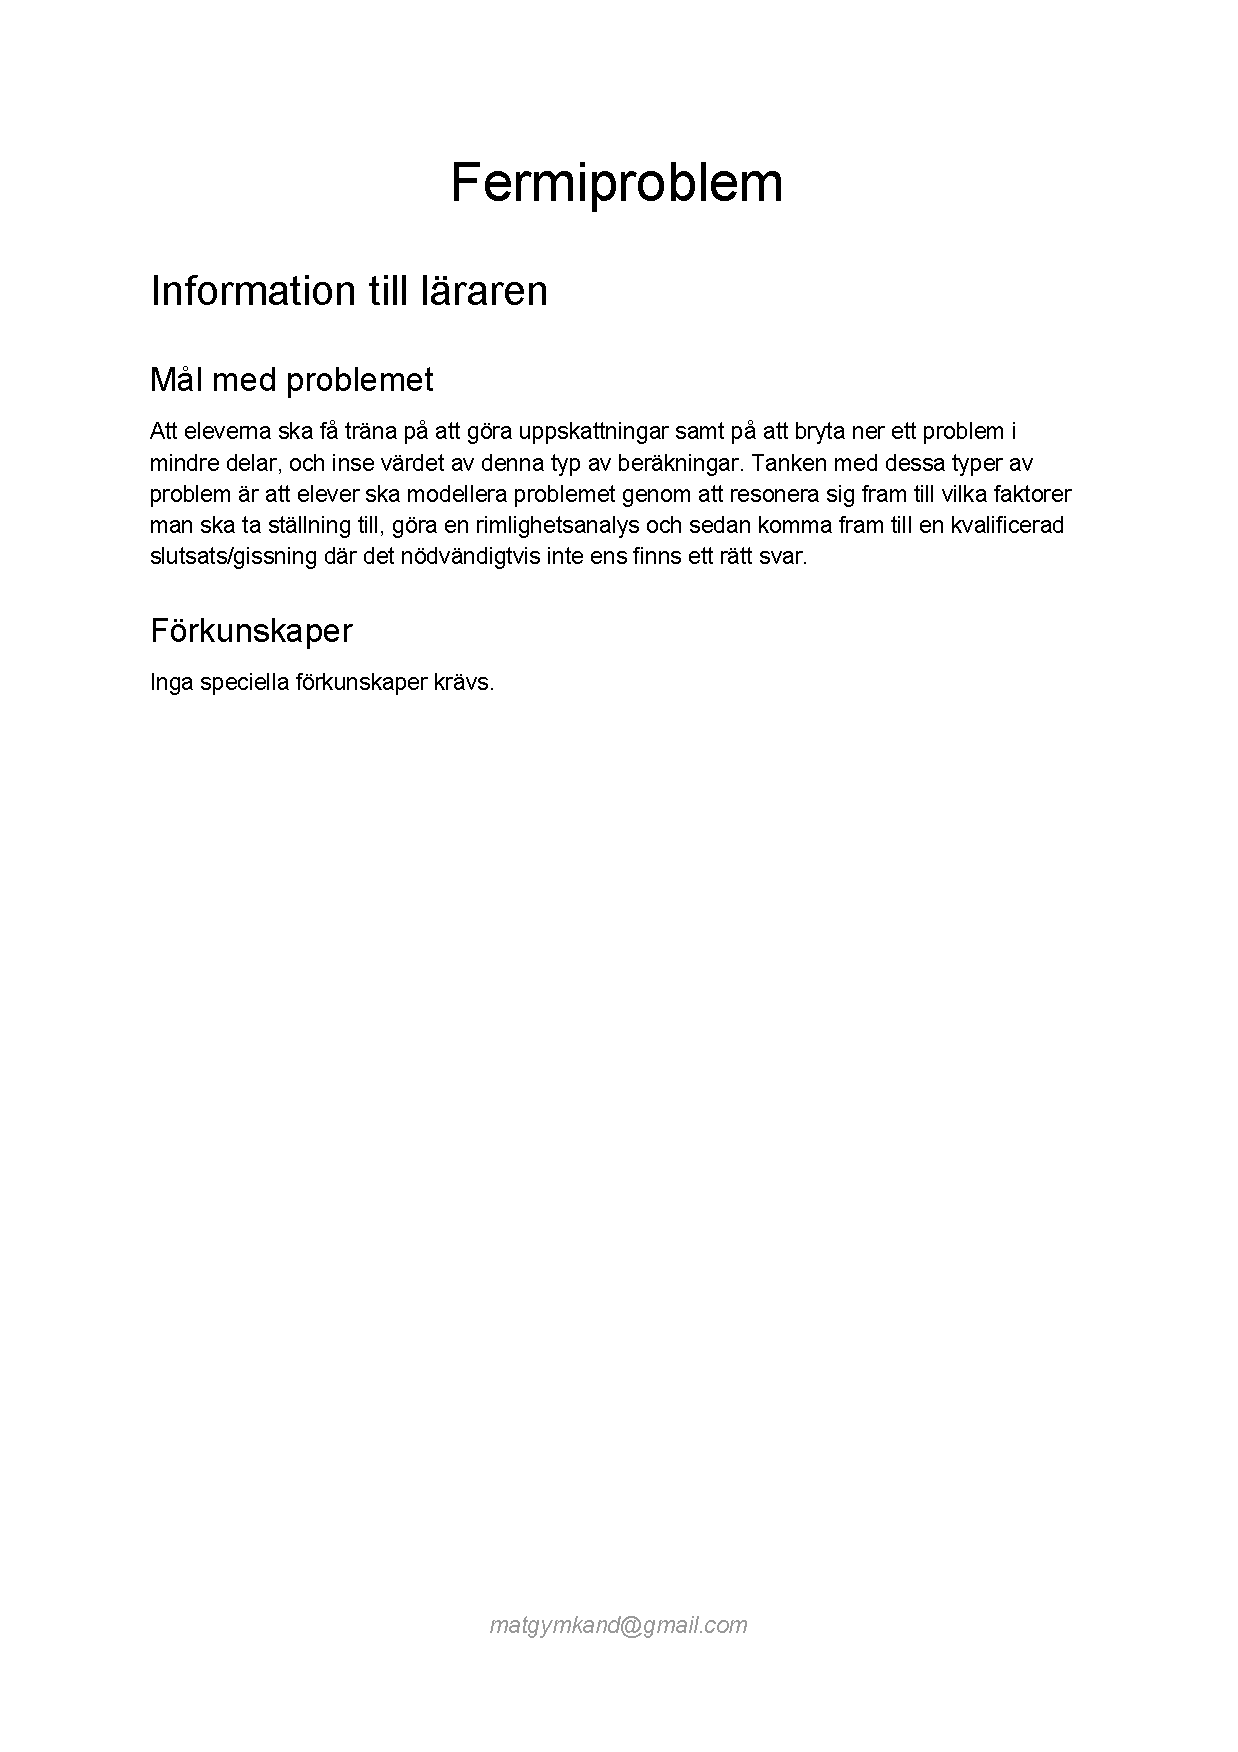
\includepdf[templatesize={210mm}{390mm}, noautoscale=true, pages=1, scale=1, pagecommand=\section{Den fullständiga versionen av problemen}\subsection{Fermiproblem}\label{app:problemen}]{Appendix/Problem/Fermi.pdf}
    \includepdf[pages=2]{Appendix/Problem/Fermi.pdf}
    \includepdf[pages=3]{Appendix/Problem/Fermi.pdf}
    \includepdf[pages=4]{Appendix/Problem/Fermi.pdf}
    
    %\subsection{Flygplan}
    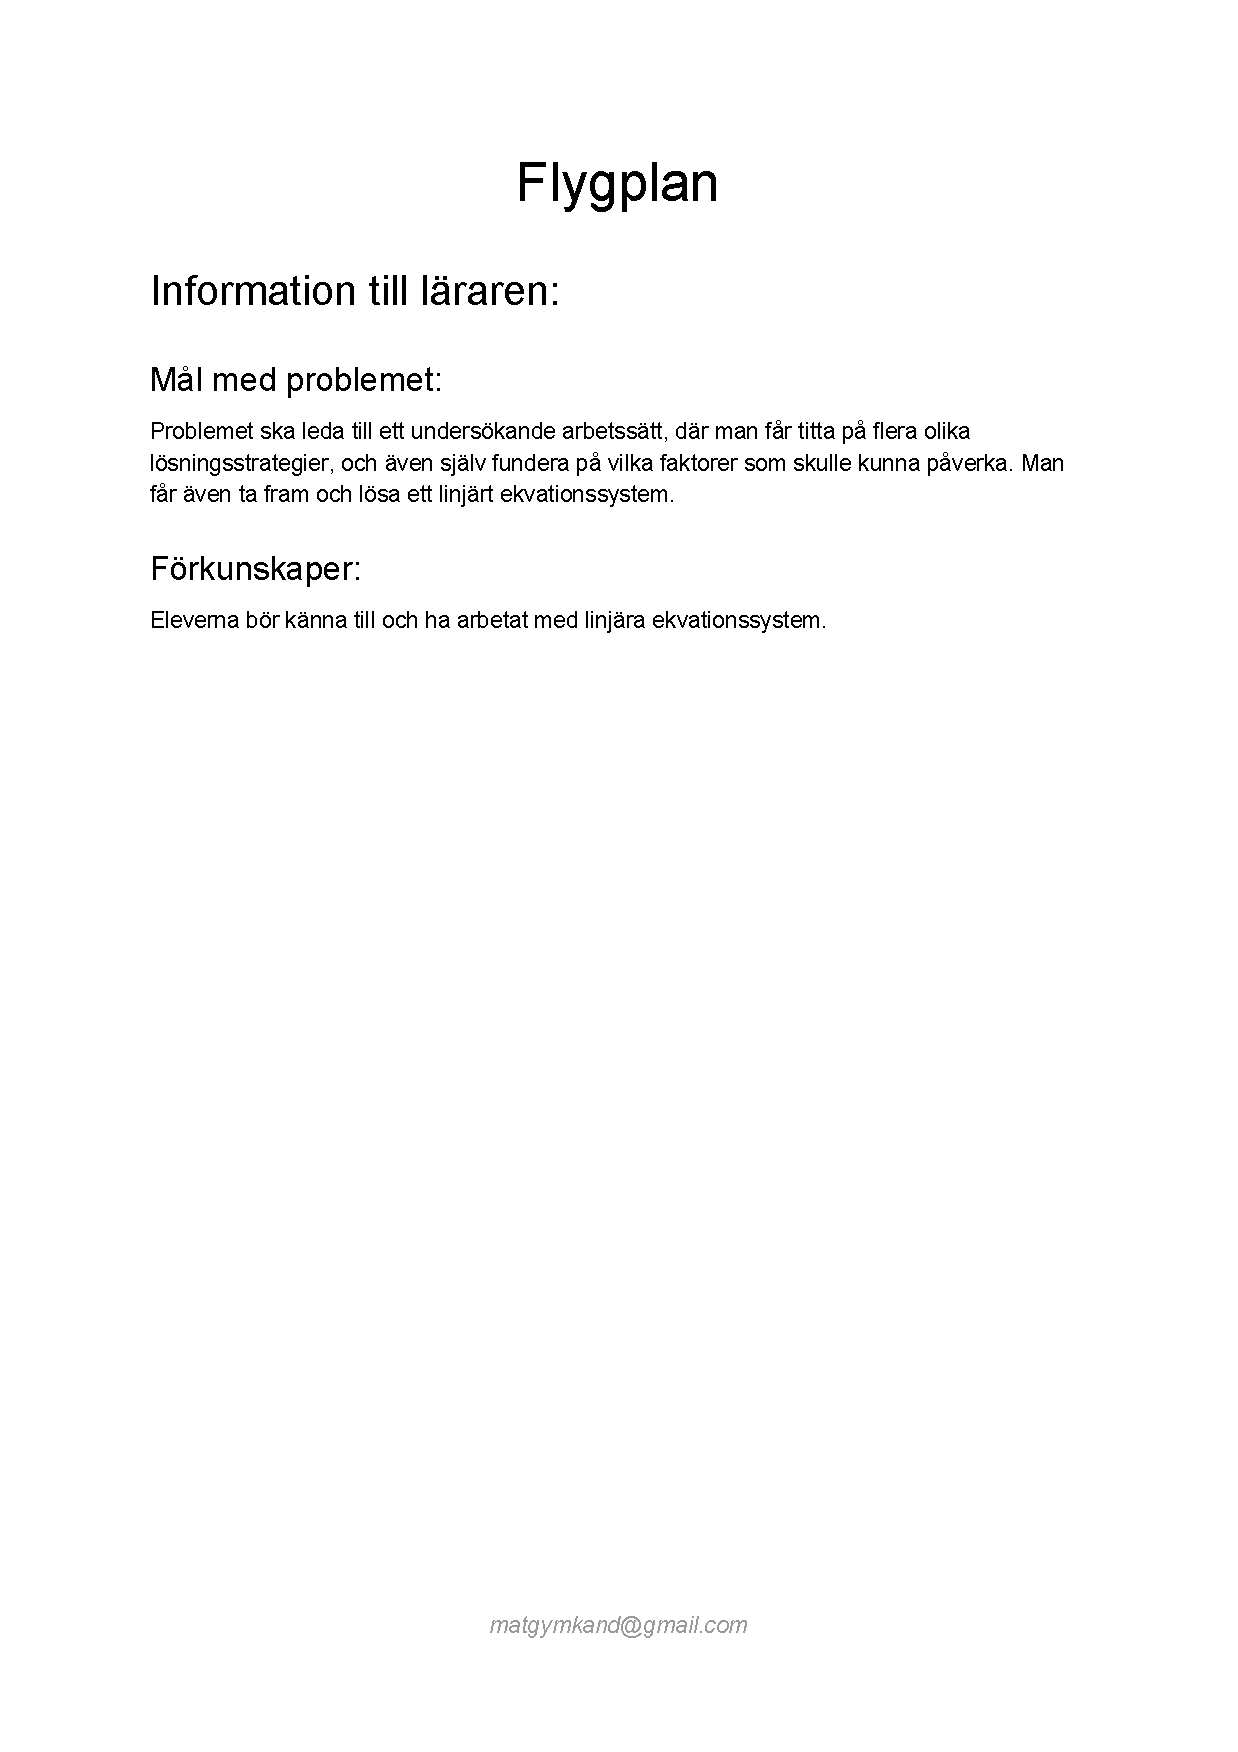
\includepdf[pages=1, templatesize={210mm}{370mm}, noautoscale=true, pages=1, scale=1, pagecommand=\subsection{Flygplan}]{Appendix/Problem/Flygplan.pdf}
    \includepdf[pages=2]{Appendix/Problem/Flygplan.pdf}
    \includepdf[pages=3]{Appendix/Problem/Flygplan.pdf}
    \includepdf[pages=4]{Appendix/Problem/Flygplan.pdf}
        
    %\subsection{Fritt fall}
    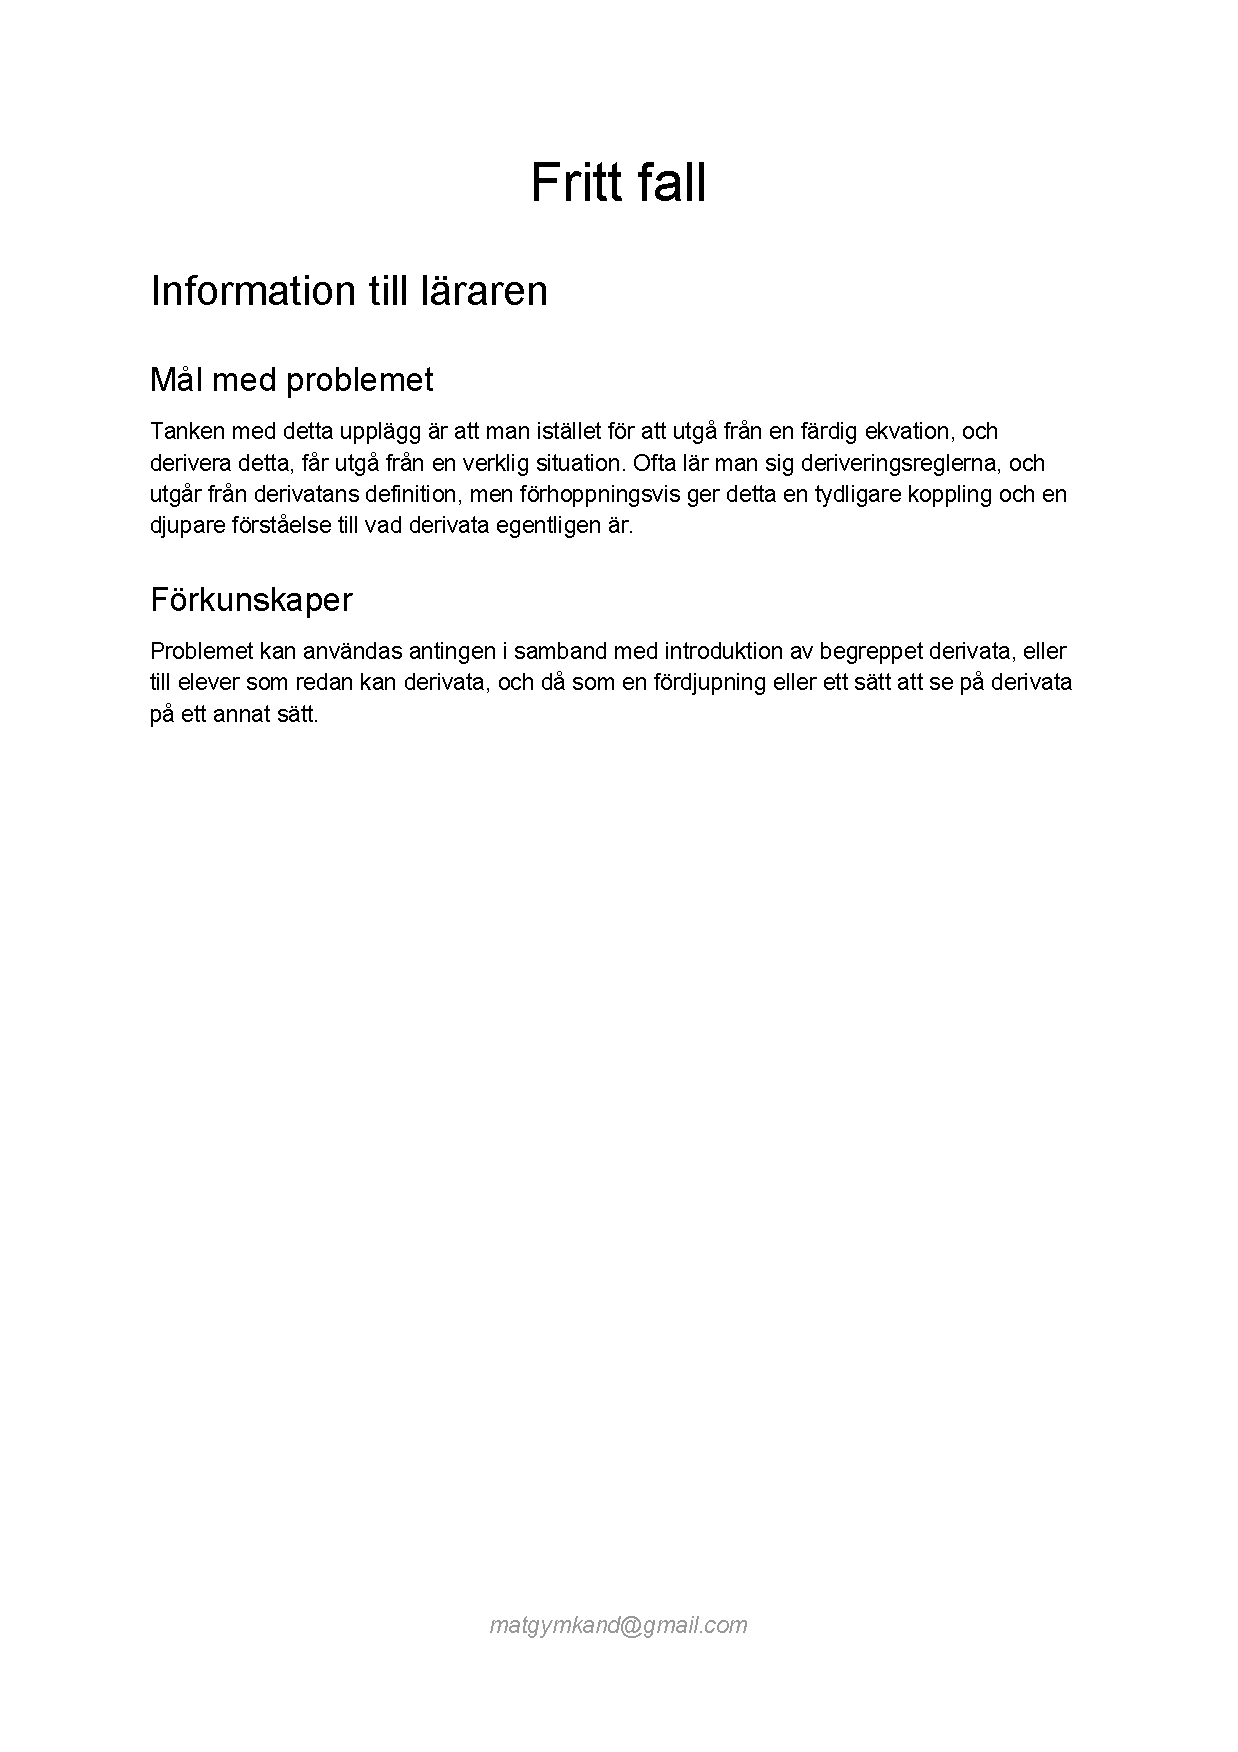
\includepdf[pages=1, templatesize={210mm}{370mm}, noautoscale=true, pages=1, scale=1, pagecommand=\subsection{Fritt fall}]{Appendix/Problem/Frittfall.pdf}
    \includepdf[pages=2]{Appendix/Problem/Frittfall.pdf}
    \includepdf[pages=3]{Appendix/Problem/Frittfall.pdf}
    
    %\subsection{Försvåring av en ekvation}
        %\includepdfmerge[nup=2x2] {Appendix/Problem/Ekvation.pdf, 1-4}
    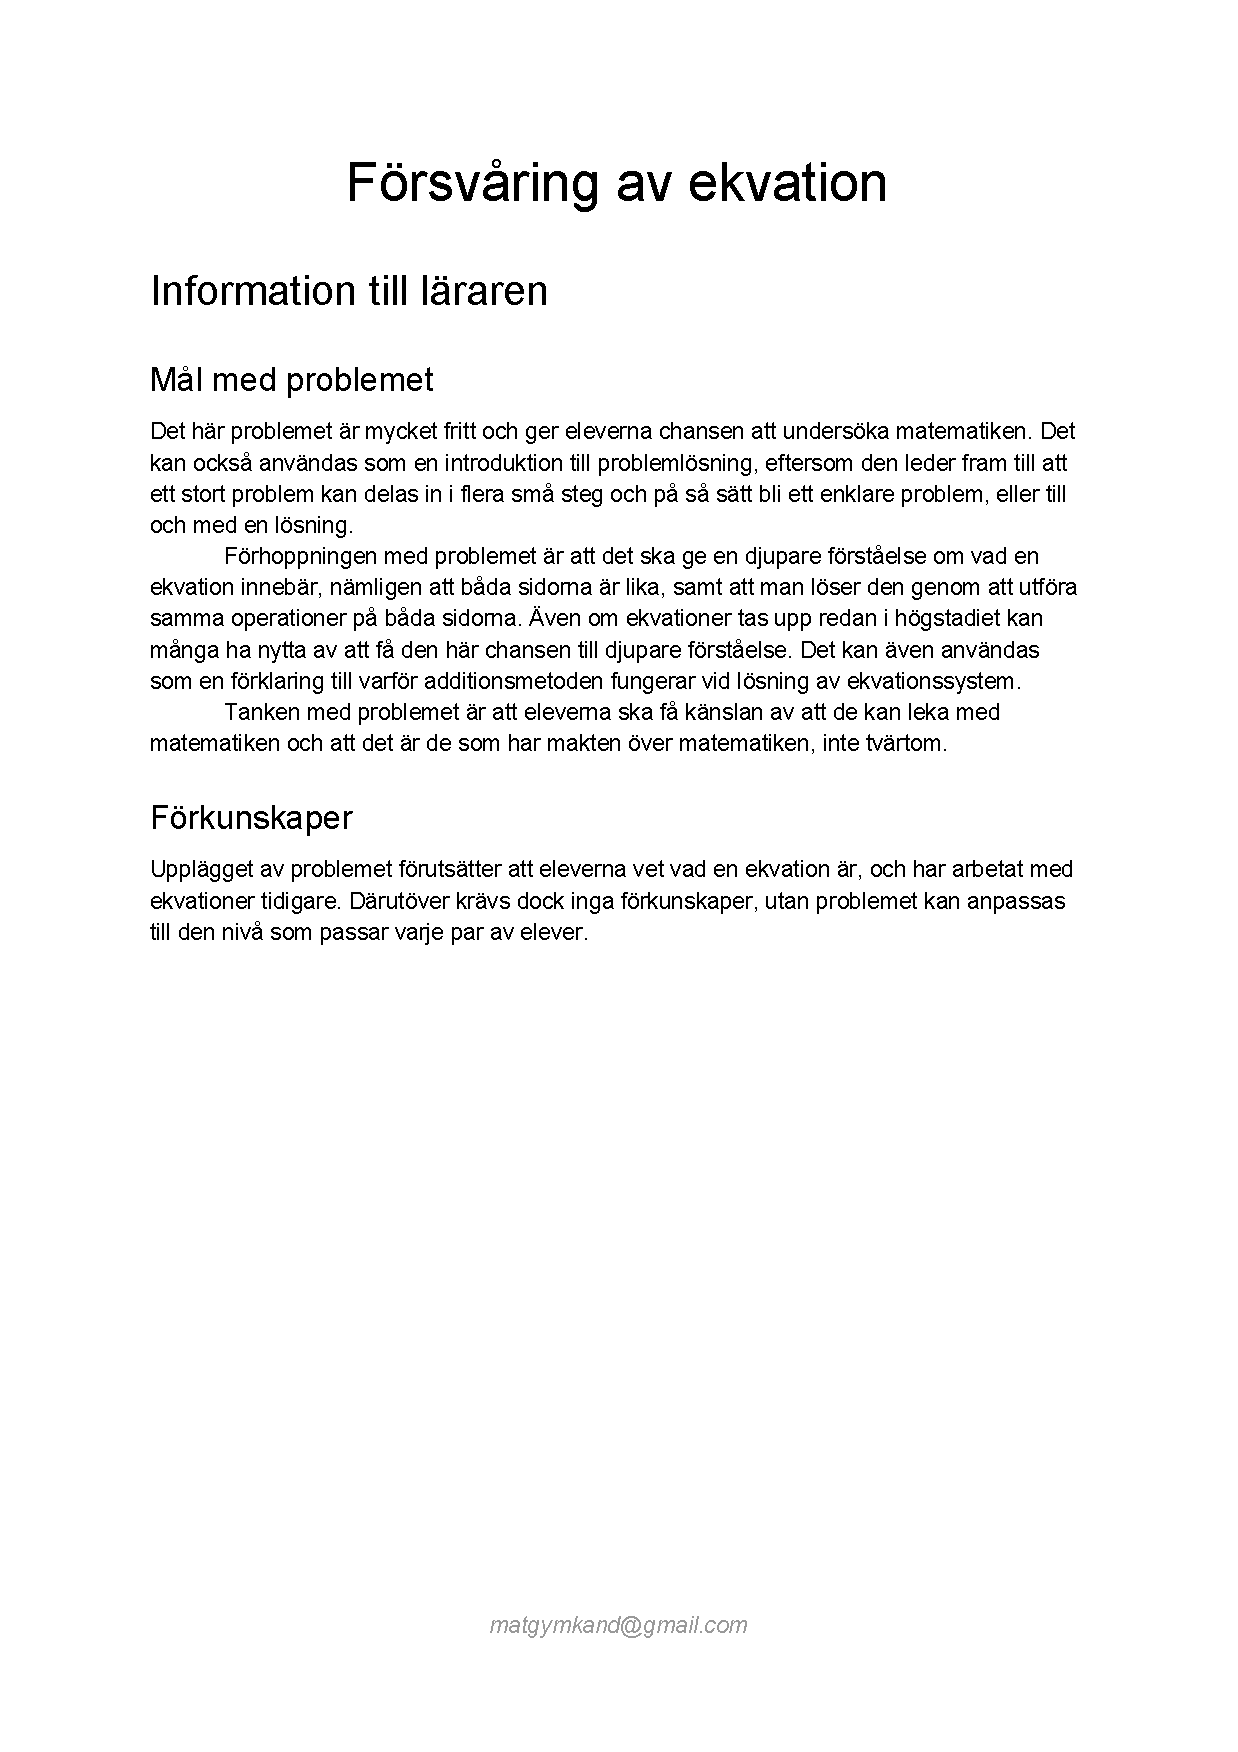
\includepdf[pages=1, templatesize={210mm}{370mm}, noautoscale=true, pages=1, scale=1, pagecommand=\subsection{Försvåring av en ekvation}]{Appendix/Problem/Ekvation.pdf}
    \includepdf[pages=2]{Appendix/Problem/Ekvation.pdf}
    \includepdf[pages=3]{Appendix/Problem/Ekvation.pdf}
    \includepdf[pages=4]{Appendix/Problem/Ekvation.pdf}
    
    %\subsection{Matematisk modell för bil och löpare}
    %    \includepdfmerge[nup=2x2] {Appendix/Problem/Lopare.pdf, 1-3}
    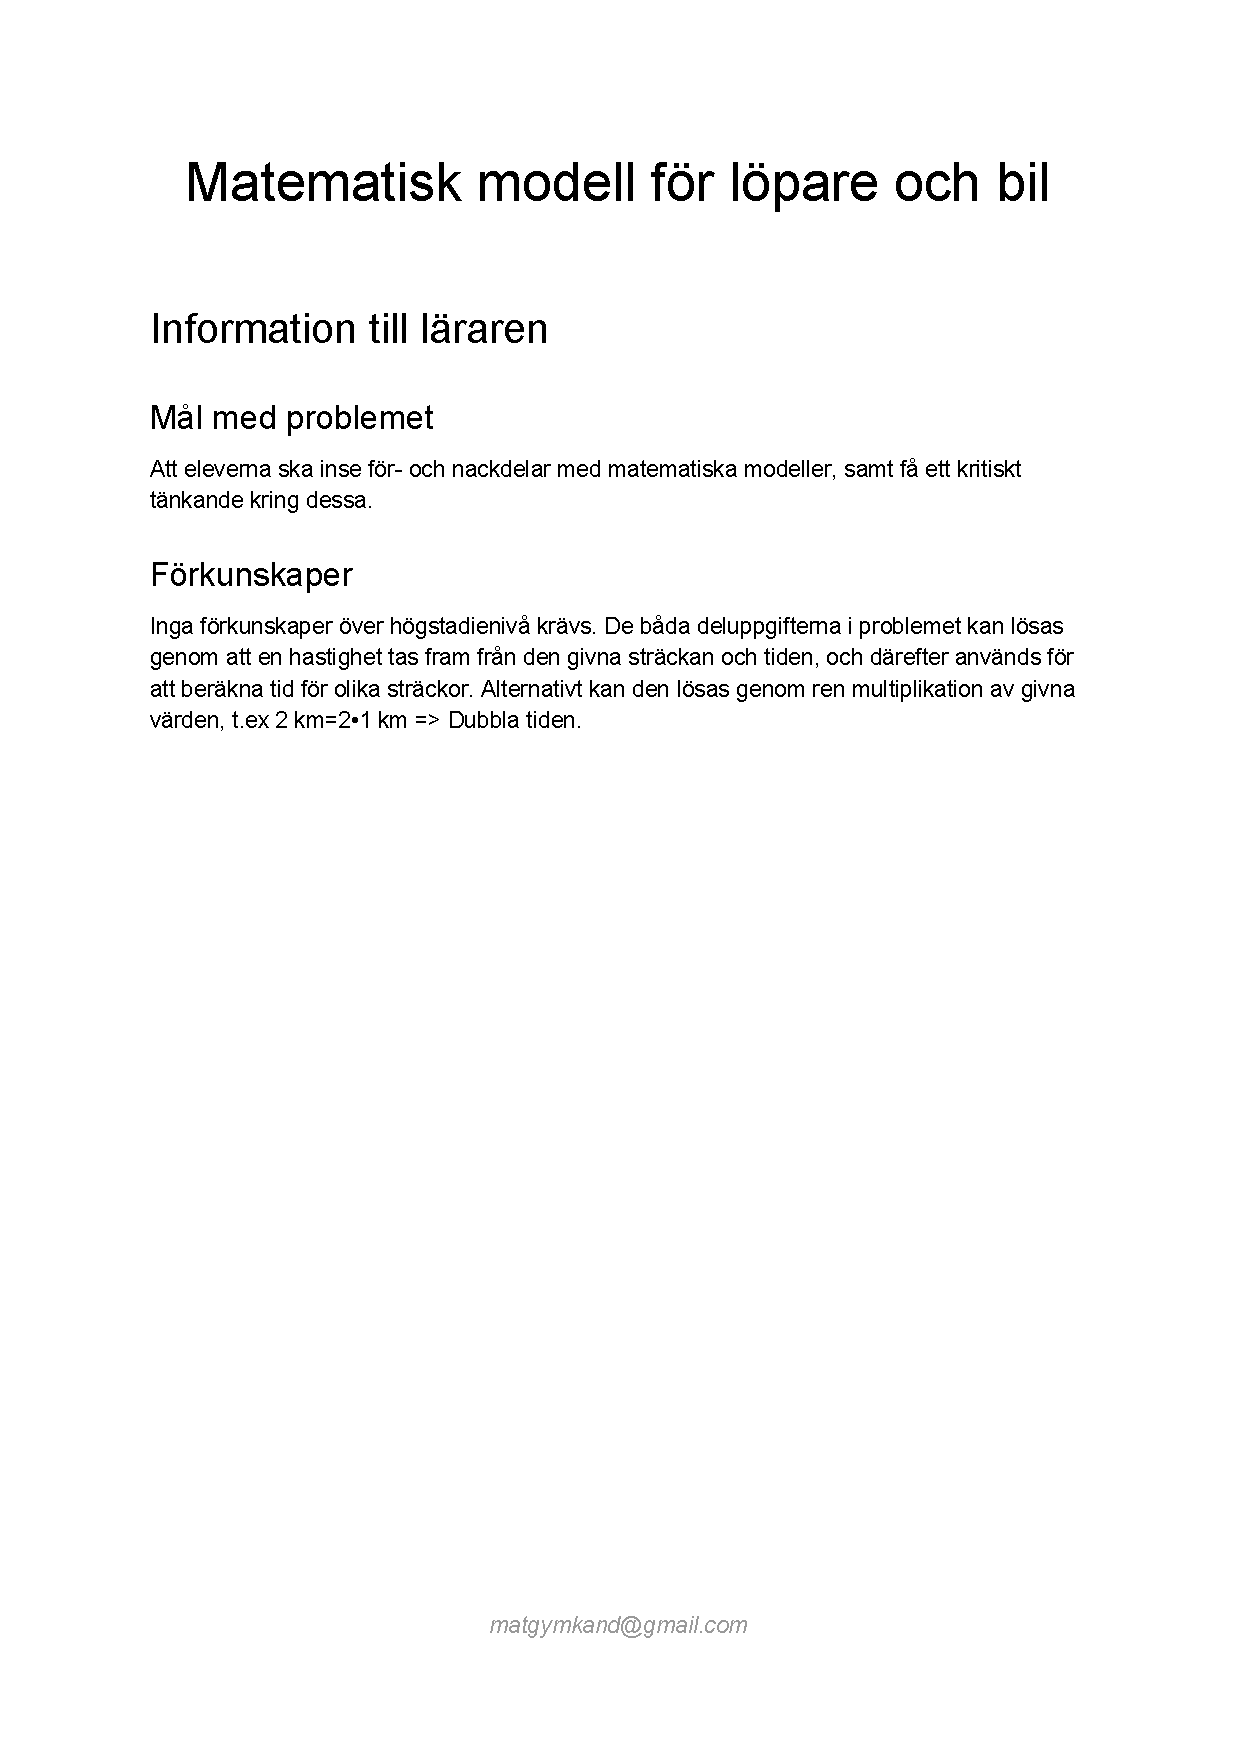
\includepdf[pages=1, templatesize={210mm}{370mm}, noautoscale=true, pages=1, scale=1, pagecommand=\subsection{Matematisk modell för bil och löpare}]{Appendix/Problem/Lopare.pdf}
    \includepdf[pages=2]{Appendix/Problem/Lopare.pdf}
    \includepdf[pages=3]{Appendix/Problem/Lopare.pdf}
    
    %\subsection{Sortera en kortlek}
        %\includepdfmerge[nup=2x2] {Appendix/Problem/Sortera.pdf, 1-4}
    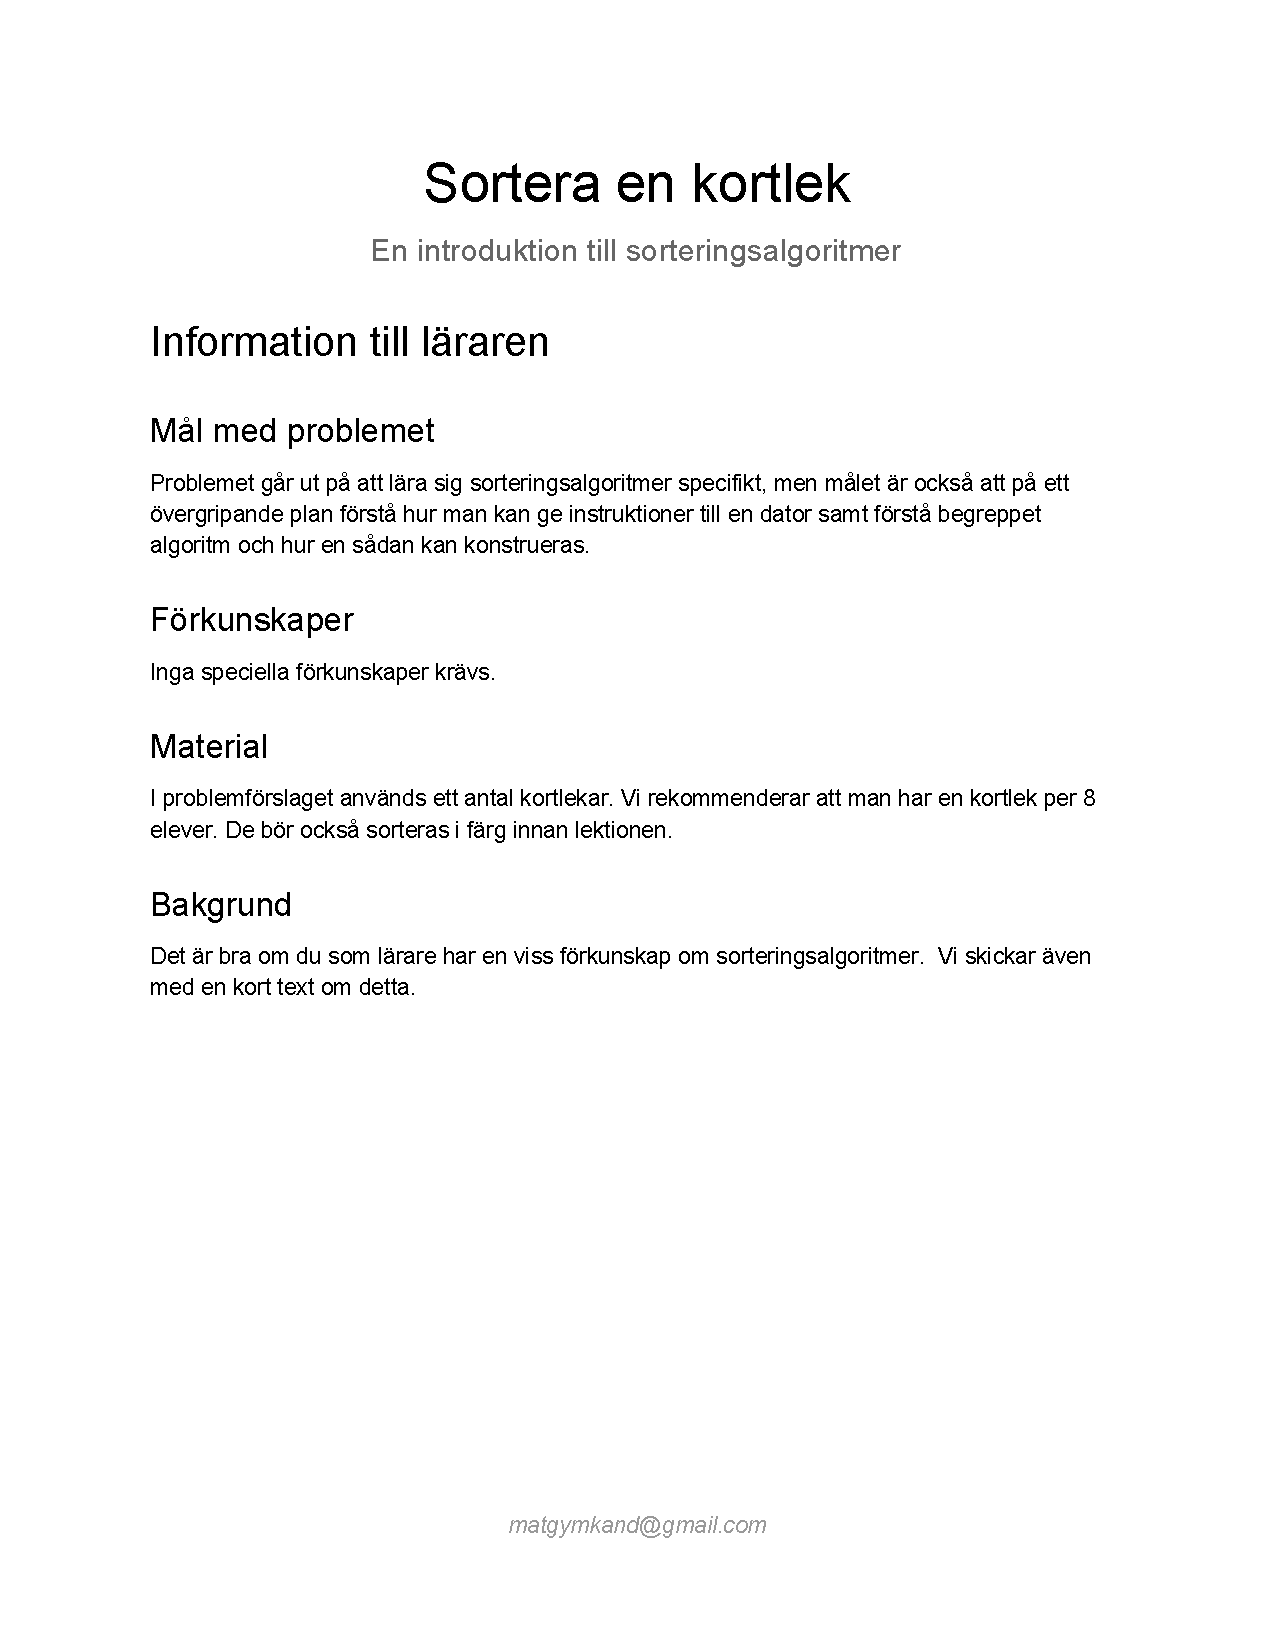
\includepdf[pages=1, templatesize={210mm}{340mm}, noautoscale=true, pages=1, scale=1, pagecommand=\subsection{Sortera en kortlek}]{Appendix/Problem/Sortera.pdf}
    \includepdf[pages=2]{Appendix/Problem/Sortera.pdf}
    \includepdf[pages=3]{Appendix/Problem/Sortera.pdf}
    \includepdf[pages=4]{Appendix/Problem/Sortera.pdf}
    
    %\subsection{Sorteringsalgoritmer}
    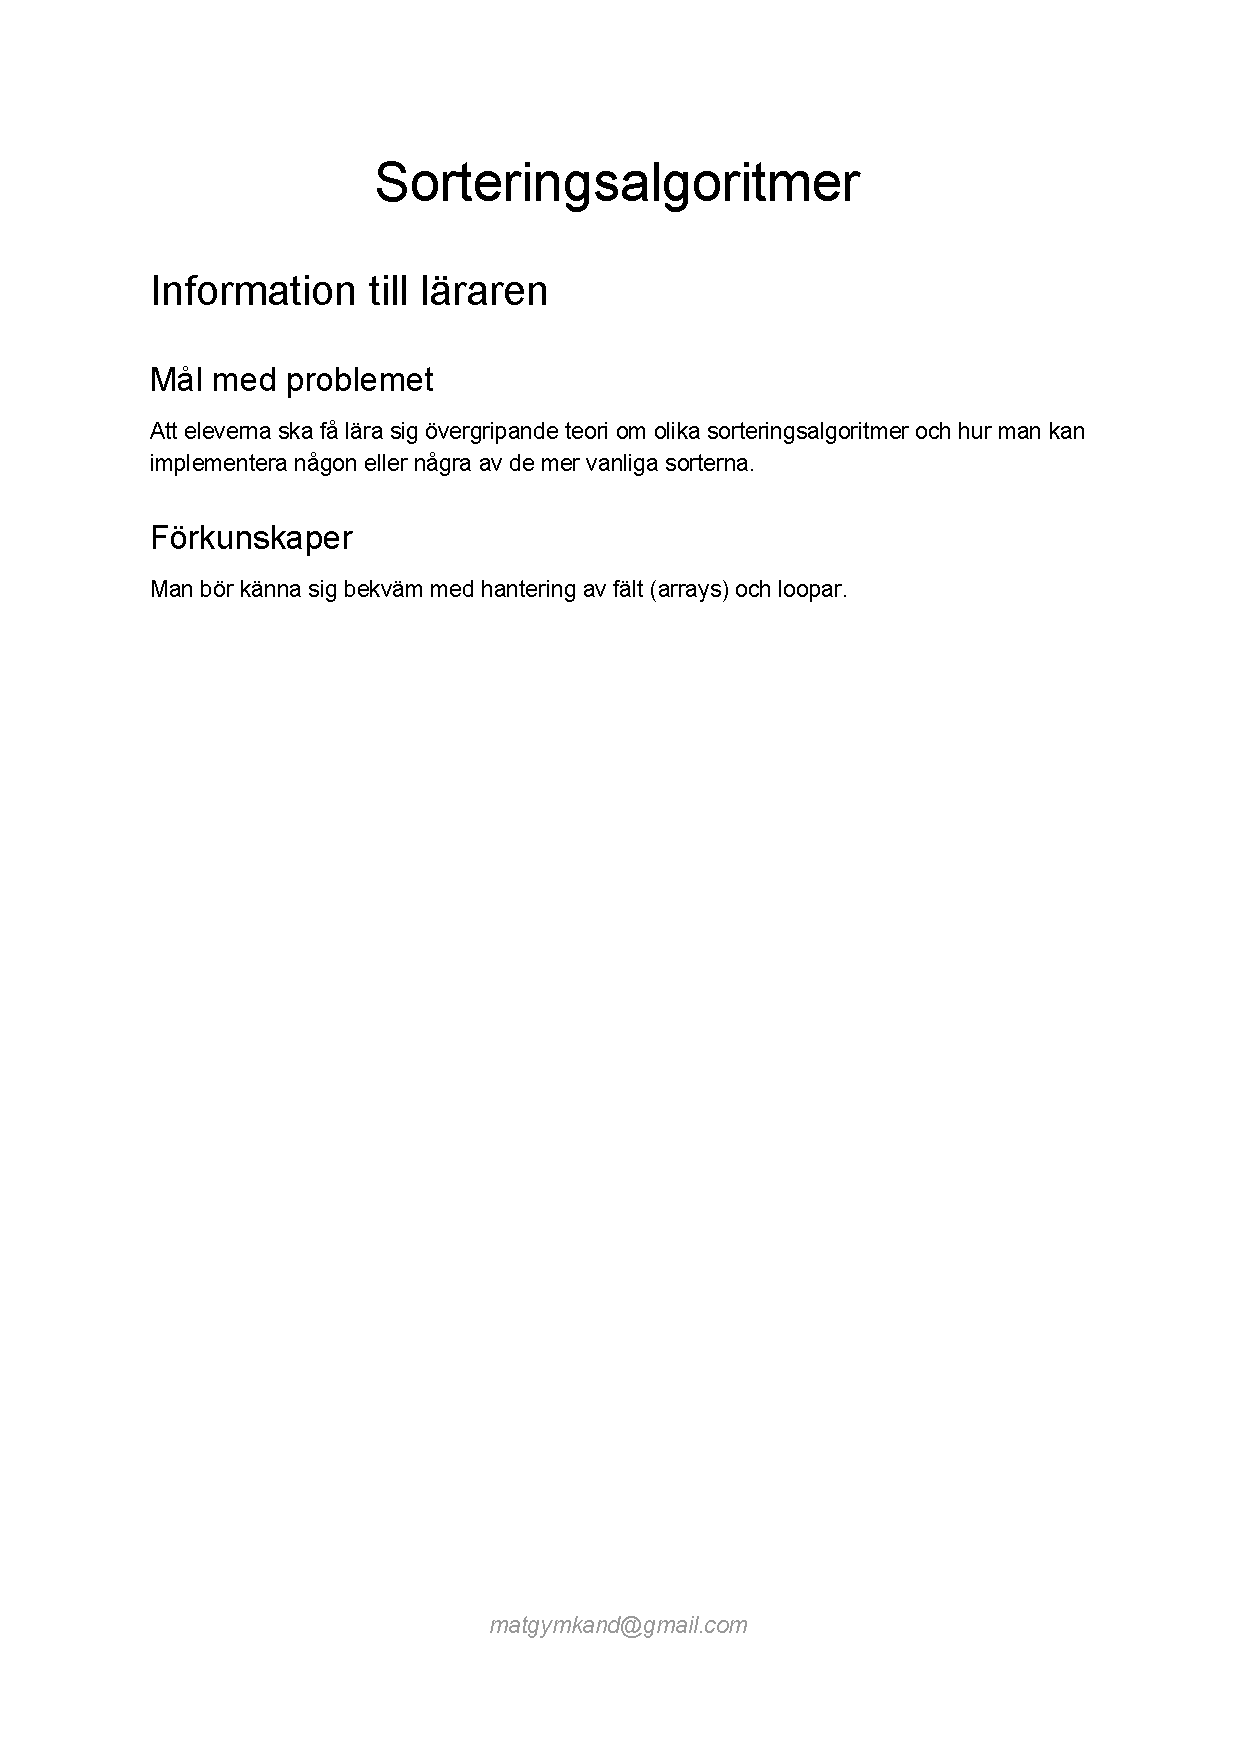
\includepdf[pages=1, templatesize={210mm}{370mm}, noautoscale=true, pages=1, scale=1, pagecommand=\subsection{Sorteringsalgoritmer}]{Appendix/Problem/Prog/Sorteringsalgoritmer.pdf}
    \includepdf[pages=2]{Appendix/Problem/Prog/Sorteringsalgoritmer.pdf}
    \includepdf[pages=3]{Appendix/Problem/Prog/Sorteringsalgoritmer.pdf}
    
    %\subsection{Approximera ett irrationellt tal}
    
\includepdf[pages=1, templatesize={210mm}{370mm}, noautoscale=true, pages=1, scale=1, pagecommand=\subsection{Approximera ett irrationellt tal}]{Appendix/Problem/Prog/Irrationellatal.pdf}
    
\includepdf[pages=2]{Appendix/Problem/Prog/Irrationellatal.pdf}
    
\includepdf[pages=3]{Appendix/Problem/Prog/Irrationellatal.pdf}   
    %\subsection{Fibonaccis talsekvens}
    
\includepdf[pages=1, templatesize={210mm}{370mm}, noautoscale=true, pages=1, scale=1, pagecommand=\subsection{Fibonaccis talsekvens}]{Appendix/Problem/Prog/Fibonacci.pdf}
    
\includepdf[pages=2]{Appendix/Problem/Prog/Fibonacci.pdf}
    
\includepdf[pages=3]{Appendix/Problem/Prog/Fibonacci.pdf}
    
    %\subsection{Identifiera primtalsfaktorer}
    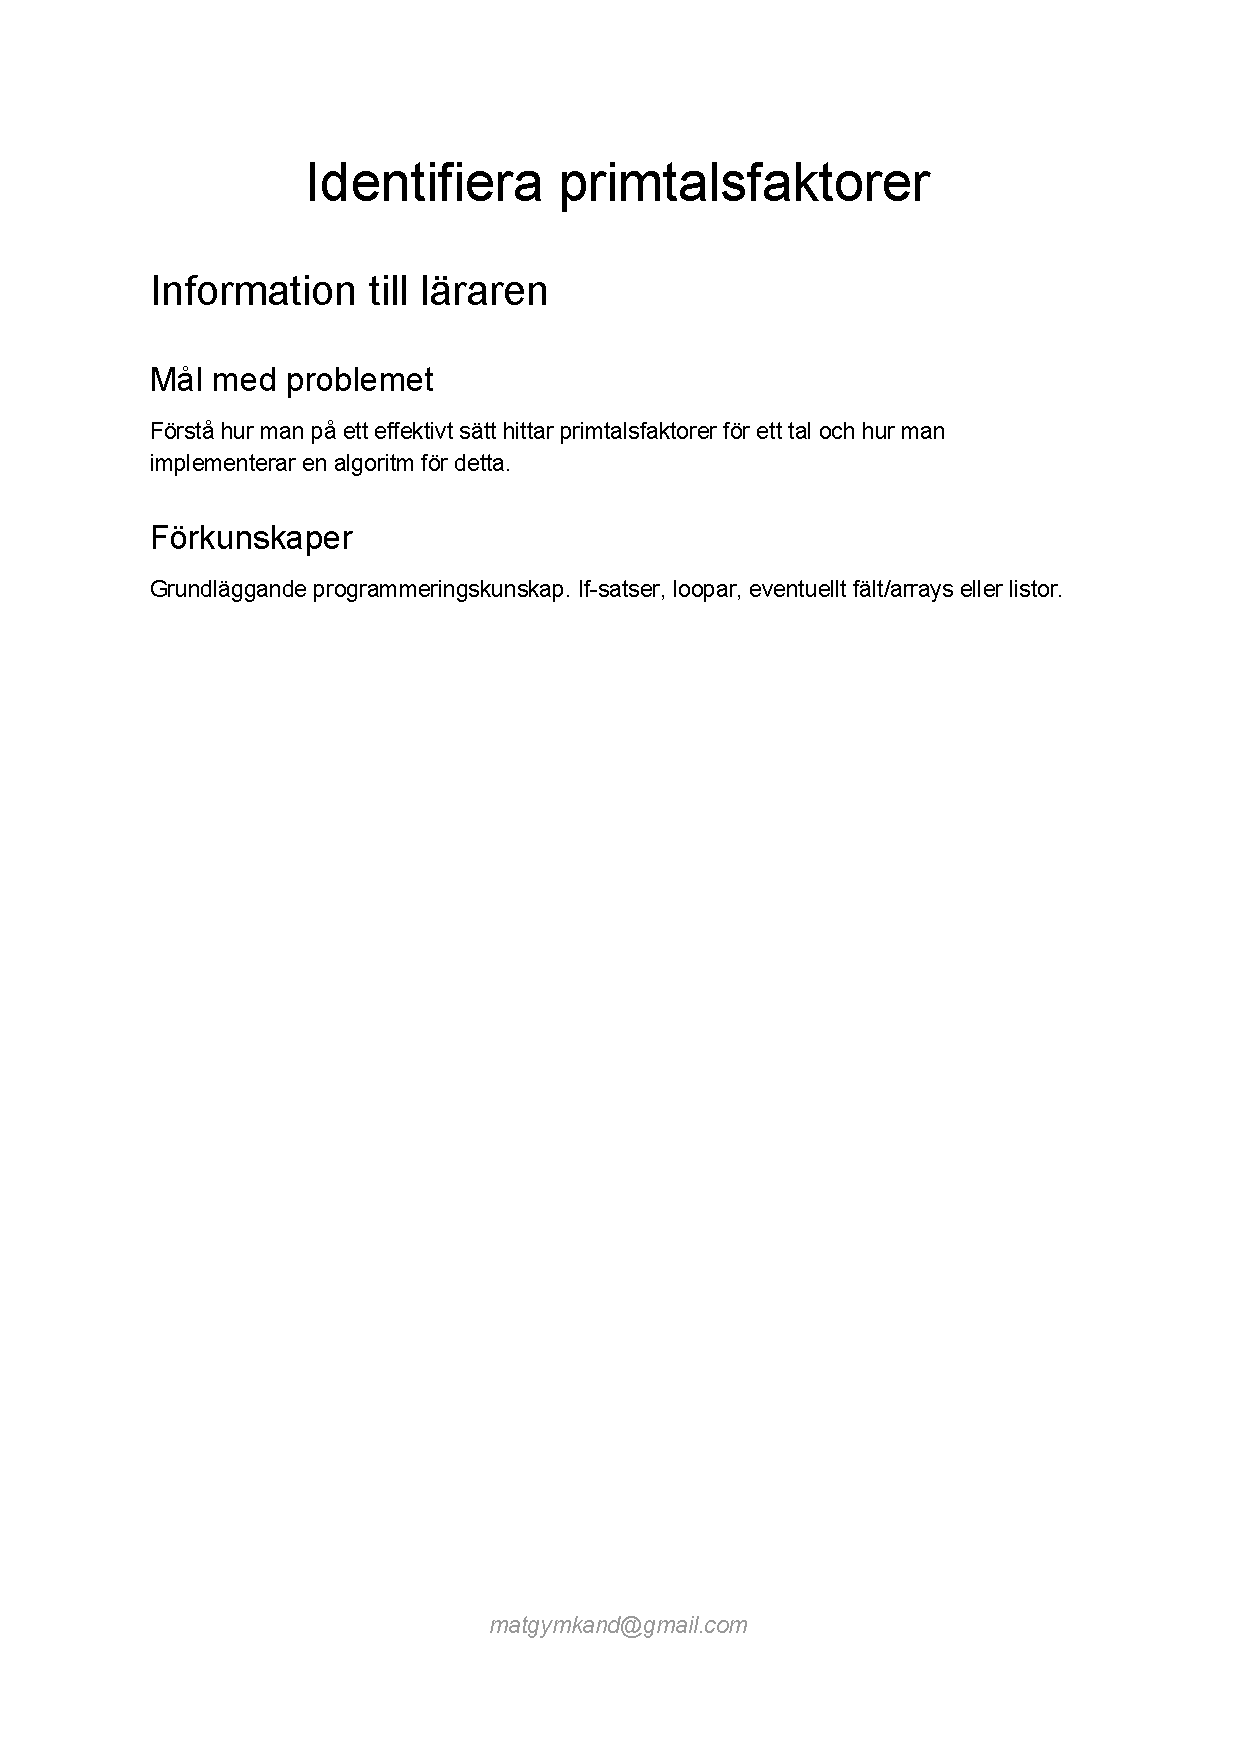
\includepdf[pages=1, templatesize={210mm}{370mm}, noautoscale=true, pages=1, scale=1, pagecommand=\subsection{Identifiera primtalsfaktorer}]{Appendix/Problem/Prog/Primtalsfaktorer.pdf}
    \includepdf[pages=2]{Appendix/Problem/Prog/Primtalsfaktorer.pdf}
    \includepdf[pages=3]{Appendix/Problem/Prog/Primtalsfaktorer.pdf}
    
    %\subsection{Personnummer}
    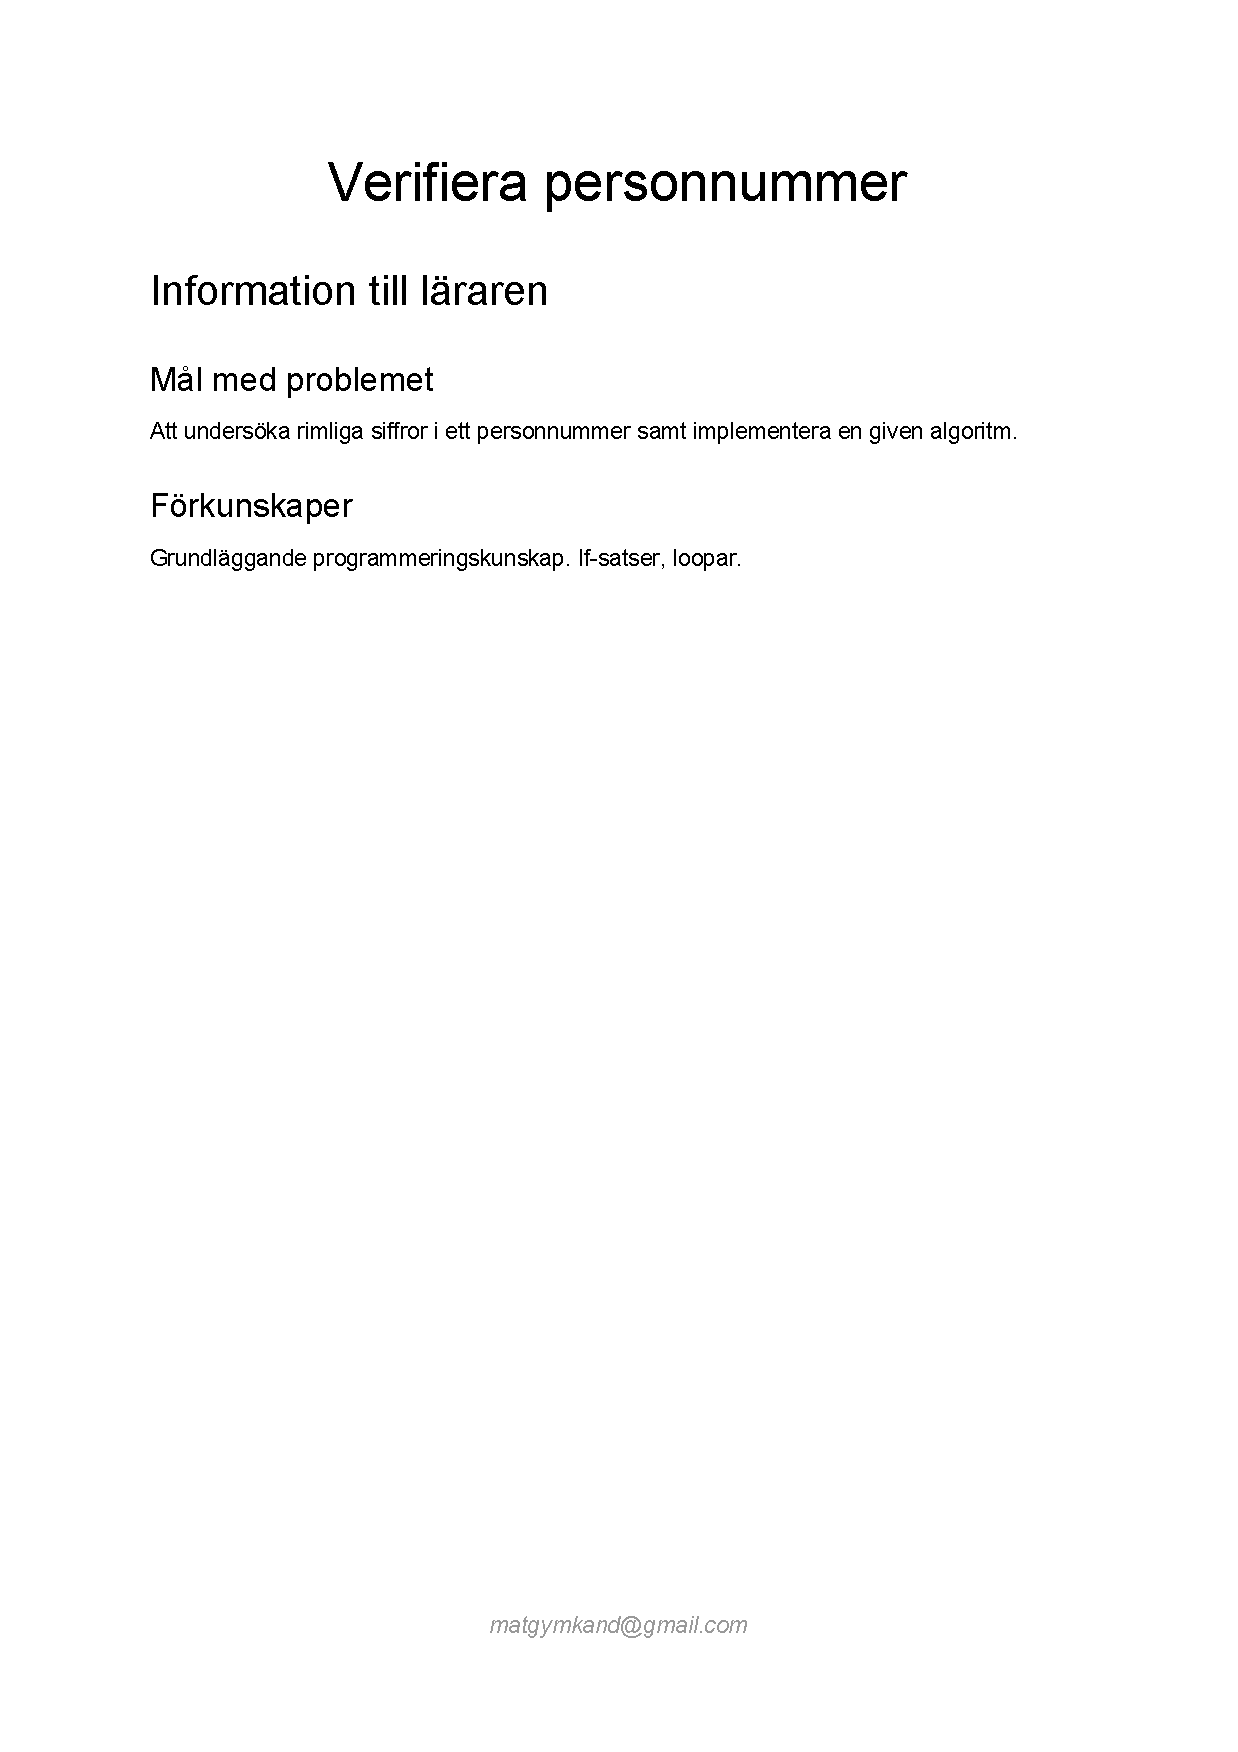
\includepdf[pages=1, templatesize={210mm}{370mm}, noautoscale=true, pages=1, scale=1, pagecommand=\subsection{Personnummer}]{Appendix/Problem/Prog/Personnummer.pdf}
    \includepdf[pages=2]{Appendix/Problem/Prog/Personnummer.pdf}
    \includepdf[pages=3]{Appendix/Problem/Prog/Personnummer.pdf}
    \includepdf[pages=4]{Appendix/Problem/Prog/Personnummer.pdf}
    
    %\subsection{Skapa ett chiffer}
    
\includepdf[pages=1, templatesize={210mm}{370mm}, noautoscale=true, pages=1, scale=1, pagecommand=\subsection{Skapa ett chiffer}]{Appendix/Problem/Prog/Chiffer.pdf}
    
\includepdf[pages=2]{Appendix/Problem/Prog/Chiffer.pdf}
    
\includepdf[pages=3]{Appendix/Problem/Prog/Chiffer.pdf}
    \includepdf[pages=4]{Appendix/Problem/Prog/Chiffer.pdf}

\newpage    

%\section{Presentationerna tillhörande problemen}
    %\subsection{Fermiproblem}
        %\includepdf{Appendix/Presentationer/Fermi.pdf}
    \includepdf[scale=0.9, pagecommand=\section{Presentationerna tillhörande problemen}\subsection{Fermiproblem}]{Appendix/Presentationer/Fermi.pdf}
    
    %\subsection{Flygplan}
    \includepdf[scale=0.9,pagecommand=\subsection{Flygplan}]{Appendix/Presentationer/Flygplan.pdf}
    \includepdfmerge[nup=1x3] {Appendix/Presentationer/Flygplan.pdf, 2-4}
    \includepdfmerge[nup=1x3] {Appendix/Presentationer/Flygplan.pdf, 5-7}
    
    %\subsection{Fritt fall}
    \includepdf[scale=0.9,pagecommand=\subsection{Fritt fall}]{Appendix/Presentationer/Frittfall.pdf}
    \includepdfmerge[nup=1x2, scale=0.9] {Appendix/Presentationer/Frittfall.pdf, 2-3}
    
    %\subsection{Försvåring av en ekvation}
    \includepdf[scale=0.9,pagecommand=\subsection{Försvåring av en ekvation}]{Appendix/Presentationer/Ekvation.pdf}
    \includepdfmerge[nup=1x3] {Appendix/Presentationer/Ekvation.pdf, 2-4}
        
    %\subsection{Matematisk modell för bil och löpare}
    \includepdf[scale=0.9,pagecommand=\subsection{Matematisk modell för bil och löparen}]{Appendix/Presentationer/Lopare.pdf}
    \includepdfmerge[nup=1x2, scale=0.9] {Appendix/Presentationer/Lopare.pdf, 2-3}
    \includepdfmerge[nup=1x2, scale=0.9] {Appendix/Presentationer/Lopare.pdf, 4-5}
    
    %\subsection{Sortera en kortlek}
    \includepdf[scale=0.9,pagecommand=\subsection{Sortera en kortlek}]{Appendix/Presentationer/Sortera.pdf}
        \includepdfmerge[nup=1x3] {Appendix/Presentationer/Sortera.pdf, 2-4}
        
    %\section{Enkäter}
    %\subsection{Förundersökning - Lärare}
    \includepdf[scale=0.9, pages=1, templatesize={180mm}{240mm}, noautoscale=true,  pagecommand=\section{Enkäter}\subsection{Förundersökning - Lärare}\label{sec:bakgrundsenkat}]{Appendix/Enkater/Forundersokning-Larare.pdf}
    \includepdf[pages=2]{Appendix/Enkater/Forundersokning-Larare.pdf}
    \includepdf[pages=3]{Appendix/Enkater/Forundersokning-Larare.pdf}
    
    %\subsection{Problemutvärdering - Lärare}
    \includepdf[scale=0.9, pages=1, templatesize={230mm}{150mm}, noautoscale=true, pagecommand=\subsection{Problemutvärdering - Lärare}]{Appendix/Enkater/Problemutvardering-Larare.pdf}
    \includepdf[pages=2]{Appendix/Enkater/Problemutvardering-Larare.pdf}
    \includepdf[pages=3]{Appendix/Enkater/Problemutvardering-Larare.pdf}
    \includepdf[pages=4]{Appendix/Enkater/Problemutvardering-Larare.pdf}
    
    %\subsection{Problemutvärdering - Elever}
    \includepdf[scale=0.9, pages=1, templatesize={230mm}{240mm}, noautoscale=true, pagecommand=\subsection{Problemutvärdering - Elever}]{Appendix/Enkater/Problemutvardering-Elever.pdf}
    \includepdf[pages=2]{Appendix/Enkater/Problemutvardering-Elever.pdf}
%    \includepdf[pages=3]{Appendix/Enkater/Problemutvardering-Elever.pdf}

\end{document}